% For hyperlinked PDF, suitable for viewing on a computer, use this:
\documentclass[letterpaper,12pt,titlepage,oneside,final]{book}

% For PDF suitable for double-sided printing, use this:
%\documentclass[letterpaper,12pt,titlepage,openright,twoside,final]{book}

\newcommand{\package}[1]{\textbf{#1}} % package names in bold text
\newcommand{\cmmd}[1]{\textbackslash\texttt{#1}} % command name in tt font
\newcommand{\href}[1]{#1}

\pdfminorversion=7  % required to convert some EPS graphics

% This package allows if-then-else control structures.
\usepackage{xifthen}
\newboolean{PrintVersion}
\setboolean{PrintVersion}{false}

\usepackage{amsmath,amssymb,amstext,amsthm}
\usepackage[pdftex]{graphicx}
\usepackage[dvipsnames,hyperref]{xcolor}
\usepackage{microtype}
\usepackage[round]{natbib}
\usepackage{rotating}
\usepackage{multicol}
\usepackage{booktabs}
\usepackage[colorinlistoftodos,prependcaption,textsize=small]{todonotes}
\newcommand{\TODO}[1]{} %{\todo[inline,backgroundcolor=blue!25]{#1}}
\usepackage{thmtools}

\usepackage{CJKutf8}  % chinese typesetting
\usepackage{listings}
\usepackage{color}
\usepackage{numprint}  % for comma separators in numbers
\npthousandsep{,}
\npthousandthpartsep{}
\npdecimalsign{.}

\usepackage{subcaption}  % for subfigure
\usepackage{mathtools}  % for Aboxed and dcases
\usepackage{textcomp} % for degree
\usepackage{multirow} % for results table
\usepackage{siunitx} % for si units
\usepackage{epstopdf} % for EPS graphics
\usepackage{tabularx} % for tabularx
\usepackage{pbox} % for pbox
\newcolumntype{Y}{>{\raggedright\arraybackslash}X}

% Set figure directories
\graphicspath{{../figures/}}

% Custom hyphenation
\hyphenation{re-arranged}

% Includes a figure. Usage:
%
% \fig{filename}{width}{caption}{shortcaption}
%
% - Filename will be used as label
% - Width is in proportion of column width
% - Shortcaption is optional
\newcommand{\fig}[4]{
  \begin{figure}[ht!]
    \centering
    \includegraphics[width=#2\columnwidth]{#1}
    \ifthenelse{\isempty{#4}}{\caption{#3}}{\caption[#3]{#4}}
    \label{fig:#1}
  \end{figure}}

% Font stuff
\usepackage{inconsolata}
\usepackage{fourier}
\usepackage[T1]{fontenc}

% https://tex.stackexchange.com/questions/67881/resetting-mathcal-font-to-default
\DeclareMathAlphabet{\mathcal}{OMS}{cmsy}{m}{n}

% argmin and argmax aren't normal?
\DeclareMathOperator*{\argmin}{arg\,min}
\DeclareMathOperator*{\argmax}{arg\,max}
\newcommand*{\bigoh}[1]{\mathcal{O}\left({#1}\right)}
\newcommand*{\laplace}[1]{\mathcal{L}\left\{{#1}\right\}}
\newcommand*{\invlaplace}[1]{\mathcal{L}^{-1}\left\{{#1}\right\}}
\newcommand*{\expect}[1]{\mathbb{E}\left[{#1}\right]}
\newcommand*{\variance}[1]{\mathbb{V}\left[{#1}\right]}

\newcommand*{\V}[1]{\mathbf{#1}}
\newcommand*{\dt}{\texttt{dt}}
\newcommand*{\IFF}{\ \iff{}\ }
\newcommand*{\transpose}[1]{{#1}^\mathsf{T}}
\newcommand*{\floor}[1]{\lfloor {#1} \rfloor}
\newcommand*{\coords}[2]{\left\{ #1 \right\}_{#2}}
\newcommand*{\ztrans}[1]{\mathcal{Z} \left\{ #1 \right\}}

% https://tex.stackexchange.com/questions/33538/how-to-get-an-approximately-proportional-to-symbol
\newcommand{\appropto}{\mathrel{\vcenter{
  \offinterlineskip\halign{\hfil$##$\cr
    \propto\cr\noalign{\kern2pt}\sim\cr\noalign{\kern-2pt}}}}}


% binding
\newcommand*{\bind}{\circledast}
% We got room; big summations please!
\everymath{\displaystyle}

\newcommand{\block}[1]{\begin{adjustwidth}{0.6cm}{}{#1}\end{adjustwidth}}

% https://tex.stackexchange.com/questions/199375/problem-with-listings-package-for-python-syntax-coloring
\DeclareFixedFont{\ttb}{T1}{txtt}{bx}{n}{9} % for bold
\DeclareFixedFont{\ttm}{T1}{txtt}{m}{n}{9}  % for normal
\definecolor{deepblue}{rgb}{0,0,0.5}
\definecolor{deepred}{rgb}{0.6,0,0}
\definecolor{deepgreen}{rgb}{0,0.5,0}
\newcommand\pythonstyle{\lstset{
  language=Python,
  backgroundcolor=\color{white}, %%%%%%%
  basicstyle=\ttm,
  otherkeywords={self},            
  keywordstyle=\ttb\color{deepblue},
  emph={MyClass,__init__},          
  emphstyle=\ttb\color{deepred},    
  stringstyle=\color{deepgreen},
  commentstyle=\color{red},  %%%%%%%%
  frame=tb,                         
  showstringspaces=false            
}}
\lstnewenvironment{python}[1][]{
  \pythonstyle
  \lstset{#1}
}{}

\newtheorem{theorem}{Theorem}[section]
\newtheorem{corollary}{Corollary}[theorem]
\newtheorem{lemma}[theorem]{Lemma}
\theoremstyle{definition}
\newtheorem{definition}{Definition}[section]

% For fancy boxes
\usepackage{tikz}
\usetikzlibrary{shapes,decorations,fit,arrows}
\tikzstyle{roundbox}=[draw=black!80, very thick,
    rectangle, rounded corners, inner sep=10pt, inner ysep=20pt]
\tikzstyle{fancytitle}=[fill=black!80, text=white]
\newcommand{\probbox}[1]{%
  \begin{center}
    \begin{tikzpicture}
      \node [roundbox] (box){%
        \begin{minipage}{0.8\textwidth}
          #1
        \end{minipage}
      };
      \node[fancytitle, right=10pt, rounded corners] at (box.north west) {%
        \textbf{Problem statement}
      };
    \end{tikzpicture}
\end{center}}
\newcommand{\inoutbox}[2]{%
  \begin{center}
    \begin{tikzpicture}
      \node [roundbox] (box){%
        \begin{minipage}{0.9\textwidth}
          \begin{multicols}{2}
            \begin{center}
              #1
              \vfill
              \columnbreak

              #2
            \end{center}
          \end{multicols}
        \end{minipage}
      };
      \node[fancytitle, right=8.4em, rounded corners] at (box.north west) {%
        \textbf{Inputs}
      };
      \node[fancytitle, left=8.2em, rounded corners] at (box.north east) {%
        \textbf{Outputs}
      };
      \draw[very thick] (box.north) -- (box.south);
    \end{tikzpicture}
\end{center}}

\tikzstyle{eblock} = [rectangle, minimum height=3em, minimum width=3em]
\tikzstyle{block} = [draw, rectangle, minimum height=3em, minimum width=3em]
\tikzstyle{sum} = [draw, circle, node distance=1cm, inner sep=0]
\tikzstyle{input} = [coordinate]
\tikzstyle{output} = [coordinate]
\tikzstyle{pinstyle} = [pin edge={to-,thin,black}]
\tikzstyle{ensemble} = [draw, circle, node distance=1cm]

% Fix error using \copyright with T1 fontenc
\renewcommand*\copyright{{\usefont{OT1}{lmr}{m}{n}\textcopyright}}

% Do this last
\usepackage[pdftex,pagebackref=false]{hyperref}
\hypersetup{
    plainpages=false,
    unicode=false,
    pdftoolbar=true,
    pdfmenubar=true,
    pdffitwindow=false,
    pdfstartview={FitH},
    pdftitle={Dynamical systems in spiking neuromorphic hardware},
    pdfauthor={Aaron R. Voelker},
    pdfsubject={Dynamical Neuromorphic Systems},
    pdfkeywords={nef} {nengo} {spiking neural networks} {dynamical systems}
                {computational neuroscience} {neuromorphics},
    pdfnewwindow=true,
    colorlinks=true,
    linkcolor=BrickRed,
    citecolor=PineGreen,
    urlcolor=cyan
}
\ifthenelse{\boolean{PrintVersion}}{
  \hypersetup{
    citecolor=black,
    filecolor=black,
    linkcolor=black,
    urlcolor=black}
}{}

\setlength{\marginparwidth}{0pt} % width of margin notes
% N.B. If margin notes are used, you must adjust \textwidth, \marginparwidth
% and \marginparsep so that the space left between the margin notes and page
% edge is less than 15 mm (0.6 in.)
\setlength{\marginparsep}{0pt} % width of space between body text and margin notes
\setlength{\evensidemargin}{0.125in} % Adds 1/8 in. to binding side of all
% even-numbered pages when the "twoside" printing option is selected
\setlength{\oddsidemargin}{0.125in} % Adds 1/8 in. to the left of all pages
% when "oneside" printing is selected, and to the left of all odd-numbered
% pages when "twoside" printing is selected
\setlength{\textwidth}{6.375in} % assuming US letter paper (8.5 in. x 11 in.) and
% side margins as above
\raggedbottom

% The following statement specifies the amount of space between
% paragraphs. Other reasonable specifications are \bigskipamount and \smallskipamount.
\setlength{\parskip}{\medskipamount}

% The following statement controls the line spacing.  The default
% spacing corresponds to good typographic conventions and only slight
% changes (e.g., perhaps "1.2"), if any, should be made.
\renewcommand{\baselinestretch}{1}

% Force each section of the front pages to start on a recto page.
% Also ensure a page number is not printed on an otherwise blank verso page.
\let\origdoublepage\cleardoublepage
\newcommand{\clearemptydoublepage}{%
  \clearpage{\pagestyle{empty}\origdoublepage}}
\let\cleardoublepage\clearemptydoublepage

\begin{document}

% suppress the page number and headers/footers.
\pagestyle{empty}
\pagenumbering{roman}

\begin{titlepage}
  \begin{center}
    \vspace*{1.0cm}

    \Huge
    {\bf Dynamical Systems in Spiking Neuromorphic Hardware}

    \vspace*{1.0cm}

    \normalsize
    by \\

    \vspace*{1.0cm}

    \Large
    Aaron Russell Voelker \\

    \vspace*{3.0cm}

    \normalsize
    A thesis \\
    presented to the University of Waterloo \\
    in fulfillment of the \\
    thesis requirement for the degree of \\
    Doctor of Philosophy \\
    in \\
    Computer Science \\

    \vspace*{2.0cm}

    Waterloo, Ontario, Canada, 2019 \\

    \vspace*{1.0cm}

    \copyright\ Aaron R. Voelker 2019 \\
  \end{center}
\end{titlepage}

% no headers, but yes page numbers (starting from ii.)
\pagestyle{plain}
\setcounter{page}{2}

\cleardoublepage

\phantomsection
\addcontentsline{toc}{chapter}{Examining Committee Membership}
\begin{center}\textbf{Examining Committee Membership}\end{center}

\noindent
The following served on the Examining Committee for this thesis.
The decision of the Examining Committee is by majority vote.

\noindent\begin{tabular}{@{}ll}\\
    External Examiner & Adrienne Fairhall \\ & Professor \\ \\
    Supervisor & Chris Eliasmith \\ & Professor \\ \\
    Internal Member & Jeff Orchard \\ & Associate Professor \\ \\
    Internal Member & Ali Ghodsi \\ & Professor \\ \\
    Internal-external Member & Sue Ann Campbell \\ & Professor
\end{tabular}

\cleardoublepage
\phantomsection
\addcontentsline{toc}{chapter}{Author's Declaration}

\noindent
This thesis consists of material all of which I authored or co-authored: see Statement of Contributions included in the thesis. This is a true copy of the thesis, including any required final revisions, as accepted by my examiners.

\bigskip

\noindent
I understand that my thesis may be made electronically available to
the public.

\cleardoublepage

\phantomsection
\addcontentsline{toc}{chapter}{Statement of Contributions}
\begin{center}\textbf{Statement of Contributions}\end{center}

\noindent
Yang Voelker provided the artwork for Figure~\ref{fig:architectures} as well as the brain illustration at the end of this front matter (the winning T-shirt design for the 2018 Telluride Neuromorphic Workshop).
Figure~\ref{fig:touch-network} was designed in collaboration with Ken E. Friedl.
Derivations from Lemma~\ref{lemma:coord-transform}, equation~\ref{eq:pulse-extended-double-exp}, and section~\ref{sec:mismatch}, extend work in collaboration with my co-authors, Kwabena Boahen and Terrence C. Stewart, both of whom provided important steps in accounting for pulse-extended double-exponential synapses with time-constant mismatch.
My advisor, Chris Eliasmith, helped author and edit several publications that have been adapted and extended throughout; references are included at the top of each applicable section.

\cleardoublepage

\phantomsection
\addcontentsline{toc}{chapter}{Abstract}
\begin{center}\textbf{Abstract}\end{center}

% The NEF is akin to a programming language for dynamical systems

\cleardoublepage

\phantomsection
\addcontentsline{toc}{chapter}{Acknowledgements}
\begin{center}\textbf{Acknowledgements}\end{center}

This thesis would not have been possible if not for my interactions with a few key people.
Most notably, my advisor, Chris Eliasmith, who gave me the freedom to swim into the deep end, and the structure, inspiration, counsel, and courage, to ask difficult, but relevant questions.
His active engagement and guidance has been instrumental throughout the development of this thesis.
Next, Terry Stewart, who programmed the Nengo backend for Braindrop, and has been an invaluable source of support when it comes to his technical prowess, breadth of knowledge, and intuition behind constructing functional spiking networks.
In my earlier days, Trevor Bekolay, Travis DeWolf, Daniel Rasmussen, and Xuan Choo, all played critical roles as academic mentors, by facilitating my exploration of the Neural Engineering Framework and Nengo.
Likewise, Eric Hunsberger, Jan Gosmann, Peter Duggins, and Andreas St{\"o}ckel, have each given feedback and provided foundational research that has deeply influenced my work.

Special mention must go out to Kwabena Boahen, who, throughout every one of our interactions, has indescribably imparted invaluable streams of insight in his critical and uncompromising quest for answers.
Many of his questions, contributions, and comments on papers, have inevitably influenced large portions of this thesis in a subtly-pervasive but positive manner.
This extends to memorable moments with all of his students, but especially Sam Fok, Alex Neckar, and Eric Kauderer-Abrams -- it has been a privilege to take part in these collaborations.

Briefly speaking with Mike Davies, hearing his eloquent characterization of neuromorphic computing, and having his genuine support in getting Loihi into the hands of researchers, has all been integral to propelling this work.
Wilten Nicola has provided a few influential communications on double-exponential synapses and FORCE learning, while Jamie Knight and Michael Hopkins have each provided important references involving SpiNNaker and high-dimensional sampling.
The words of many others have shaped this thesis throughout.

At the institutional level, I would like to acknowledge the support that I've received from
ABR (for Nengo and NengoLib development and experimentation with Loihi),
Intel (for access to Loihi),
Femtosense (for access to and support with Braindrop),
and the University of Manchester (for access to SpiNNaker).
Likewise, my acceptance into the neuromorphic workshops of Telluride, Capo Caccia, Intel's Neuromorphic Research Community~(INRC), and the Nengo Summer School, have all proven to be constructive experiences and motivational fuel.
The Centre for Theoretical Neuroscience~(CTN), Computational Neuroscience Research Group~(CNRG), David R. Cheriton School of Computer Science, and the University of Waterloo, have all contributed to providing a supportive academic environment over the past 11 years.  

\newpage

The experiments throughout this thesis make extensive use of Python, NumPy, SciPy, Jupyter, Matplotlib, Seaborn, Pandas, Nengo, PyStorm, Hyperopt, Scitkit-learn, Keras, and TensorFlow -- for this, we are incredibly grateful to its thousands of contributors.
A repeated mention is in order for Trevor, who provided this modified \LaTeX{} template and facilitated my contributions to the Nengo software ecosystem.
Likewise, Daniel, Eric, and Jan, for their help with Nengo development, provisioning of useful code, and feedback.

Working backwards in time, I would also like to thank Mani Fazeli for his many letters of support and words of wisdom at the beginning of graduate school, as well as Carol Norman for her recurring words of encouragement.
And the enriched education that I received from my teacher Jon Devlin, at Bell High School, was monumental in my decision to study computer science at the University of Waterloo.

At a personal level, Chris has been an outstanding role model for how to live a balanced and meaningful life, as an academic, parent, and human being, all in ways that I can only aspire towards.
Jason Batten-Carew has been the source of many extended philosophical discussions centered on the nature of reality, perception, stories, games, and cycles, all of which have undoubtedly rooted their way into my most basic pursuits for meaning.
I also thank my mom and dad for exciting my curiosity, and enabling my studies, throughout my entire life.
And finally I thank my wife, Yang Peng, for providing much-needed perspective and support throughout it all.

\cleardoublepage

\phantomsection
\addcontentsline{toc}{chapter}{Dedication}
\begin{center}
  \textbf{Dedication}

  To Yang -- the love of my life.
  And to Gunter -- for he is a dog.
\end{center}

\cleardoublepage

% https://tex.stackexchange.com/questions/65544/how-to-link-table-of-contents-in-thesis-pdf
\cleardoublepage
\phantomsection
\renewcommand\contentsname{Table of Contents}
%\pdfbookmark[section]{\contentsname}{Table of Contents}
\addcontentsline{toc}{chapter}{Table of Contents}
\tableofcontents
\cleardoublepage
\phantomsection

\iffalse
\addcontentsline{toc}{chapter}{List of Todos}
\listoftodos
\cleardoublepage
\phantomsection
\fi

\addcontentsline{toc}{chapter}{List of Tables}
\listoftables
\cleardoublepage
\phantomsection

\addcontentsline{toc}{chapter}{List of Figures}
\listoffigures
\cleardoublepage
\phantomsection

\addcontentsline{toc}{chapter}{List of Theorems}
\listoftheorems[ignoreall,show={theorem,lemma}]
\cleardoublepage
\phantomsection

\chapter*{Mathematical Conventions}
\addcontentsline{toc}{chapter}{Mathematical Conventions}
\label{typography}

This thesis follows standard mathematical conventions of using lower-case italic variables~($u(t)$) to represent scalar quantities, lower-case bold variables~($\V{x}(t)$) to represent vector quantities, upper-case italic variables~($A$) to represent matrices, and Greek letters~($\tau$, $\theta$) to represent quantities with a unit of time.
Bars are included above variables ($\bar{A}$) to indicate discretization in time.
Depending on context, $F(s)$ or $F(z)$ are used to represent complex values in the Laplace $s$-domain, or digital $z$-domain, respectively.

\cleardoublepage
\phantomsection

\begin{figure}
\centering
\vspace*{\fill}
\begingroup
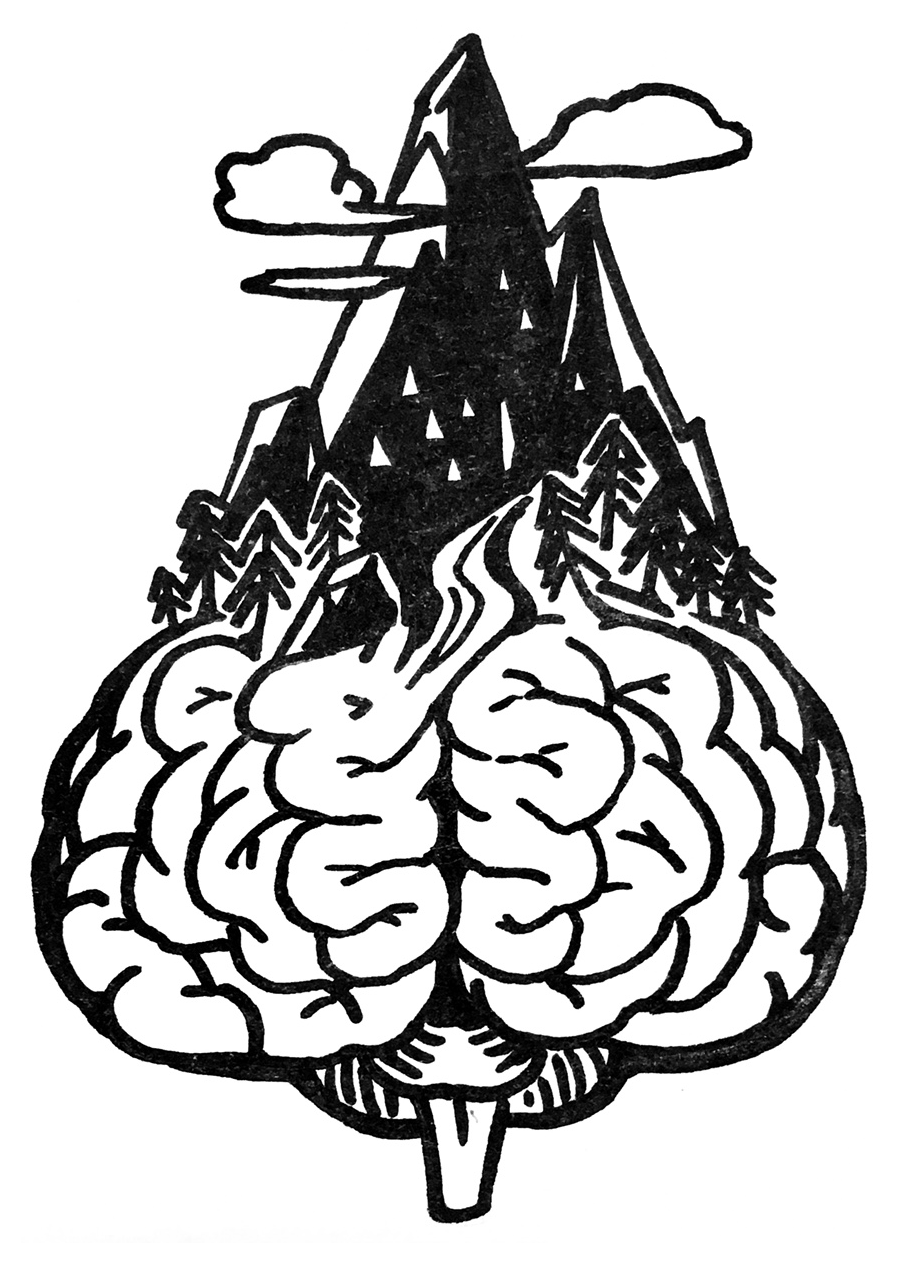
\includegraphics[width=0.6\columnwidth]{yang-peng-telluride-back-2018.png}
\endgroup

\vspace{1em} 

\caption*{{\tiny \emph{``You would say to God, `How did you make the mountains?' and he would say... `Well, you're asking me to describe in words how I made the mountains, and there are no words which can do this. Words cannot tell you how I made the mountains any more than I can drink the ocean with a fork... It would take millions of years, and you would be bored with my description, long before I got through it... because I didn't create the mountains with words, I just did it. Like you open and close your hand. You know how you do this, but can you describe in words how you do it? Even a very good physiologist can't describe it in words. But you do it. You're conscious, aren't you. Don't you know how you manage to be conscious?''}~\textasciitilde~Alan Watts}}

\vspace*{\fill}
\end{figure}

\cleardoublepage
\phantomsection

% Change page numbering back to Arabic numerals
\pagenumbering{arabic}

% https://tex.stackexchange.com/questions/32208/footnote-runs-onto-second-page
\interfootnotelinepenalty=10000

\chapter{Introduction}

Computation cannot be physically realized without time.
Whether we consider the discrete switching of voltage states across transistors in a
digital computer,
or the continuous flow of charges across ion channels within the brain -- 
all physical systems, that we currently know of, make progress on their computations
by changing over time.
Digital computers time-multiplex their computations across multiple cores with energetically-expensive access to distant memory, while our brains consume only twenty watts of power by harnessing the dynamics of a biophysical substrate.
An overarching focus of this thesis is a computational paradigm
in between these two extremes: neuromorphic computing.
Here, researchers draw inspiration from how the
brain dynamically performs computations,
to engineer low-power digital and analog circuits that emulate its fundamental principles.

The emerging field of neuromorphic computing has already
witnessed many successes backed by large companies, small start-ups, and new research
programs being established at various institutions all around the world.
Applied Brain Research (ABR), Femtosense, Intel, IBM, and many others~\citep{marketreport2018}, are establishing themselves as key players in the field, while a collaborative landscape is being fostered across a diverse set of academic communities attempting to use such hardware including the Telluride Neuromorphic Cognition Engineering Workshop~\citep{cohen2001report}, Capo Caccia Cognitive Neuromorphic Engineering Workshop, Nengo Summer School~(ABR's ``Brain Camp''), and Intel's Neuromorphic Research Community~(INRC).

Despite this growing excitement, there exist many challenges when it comes to using
neuromorphic hardware to perform some desired task.
Generally speaking, neuromorphic programming forces us to rethink our traditional,
\citet{von1958}, understanding of computation, and redesign our algorithms to leverage distributed networks of noisy, heterogeneous units, that locally process their inputs and communicate via spikes -- also known as Spiking Neural Networks~(SNNs).
Biological nervous systems already do this quite successfully, and so we seek to borrow existing
principles and models from neuroscience, exploit their properties using tools from mathematics and engineering,
and use software methods to synthesize the resulting networks ``in silico''.
Moreover, the frameworks and methods that we use to accomplish this should be extensible---willing and able to incorporate increasingly-sophisticated levels of biological detail---so long as such details are computationally useful at a functional level, or shown to benefit some resource-power-accuracy trade-off.

To what end?
By virtue of emulating core principles of brain function, this realizes algorithms that consume far less power, and scale more readily to massively-parallelized computing architectures running in biological real-time.
But such algorithms must also be practically useful.
To flip this on its head: we require frameworks to describe what some hardware is doing at the lowest level,
and tools to systematically harness its capabilities to perform useful computations at the highest level.
Analagous to how a single compiler can translate the same C++ code
to dozens of physically distinct digital architectures, we strive to systematically describe
how the same dynamical computations can be flexibly mapped onto distinct spiking neuromorphic architectures.

The primary goals of this thesis are to explore the above statements, and in doing so elucidate a general recipe for implementing efficient dynamical computations on neuromorphic hardware, empower theorists and practitioners with deeper insights into subtle relationships between network configuration and function, and finally validate this approach with practical results that include a set of novel spiking algorithms deployed on state-of-the-art neuromorphic chips: Braindrop~\citep{braindrop2019} and Loihi~\citep{davies2018loihi}.
Ultimately, this unveils a class of computations where neuromorphic hardware excels, and further automates the process of engineering algorithms for such hardware.

We have already learned a great deal through the mutually interacting processes of bottom-up neuromorphic hardware design and top-down SNN construction.
Theoretical frameworks help guide design decisions, while hardware constraints demand relevant extensions to theoretical frameworks and software tools; both processes give-and-take in a dynamic feedback loop.
Our general approach consists of a software stack, and nonlinear dynamical systems framework,
for describing computations within a language of low-frequency vector spaces.
This approach is known as the Neural Engineering Framework~\citep[NEF;][]{eliasmith2003a}.
The NEF is implemented by the Python package, Nengo~\citep{bekolay2014}, which supports a variety of neuromorphic backends, and is extended by the methods
described in this thesis.
The ultimate goal of this approach is to develop a unified set of tools for constructing
artificially intelligent agents, that scale to the same kinds of tasks that
humans can perform, while running on neuromorphic hardware consuming several orders of magnitude less power than a traditional computer.
Significant progress has been made in this direction over the past two decades -- and although we still
have a long ways to go, this thesis aims to highlight a promising path for the neuromorphic community.

When confronted with the ambitious goal of artificially reproducing human intelligence, computer scientists will most often point towards
the popularity of deep learning~\citep{lecun2015deep} and its recent successes such as AlphaGo~\citep{gibney2016google}.
First and foremost, we seek to embrace the methods of deep learning, by incorporating its architectures and training methodoligies into our toolbox.
This is in fact the mandate of Nengo DL~\citep{rasmussen2018nengodl}, a Python package that combines Nengo and Tensorflow into a hybridized framework that automates backpropagation across spiking, non-spiking, and NEF-style recurrent neural networks -- broadly referred to as the class of Artificial Neural Networks~(ANNs).
Deep learning methods have found enormous success, due in part to the black-box nature of its training procedure, which requires a programmer to have virtually no knowledge of the underlying problem being solved.
However, we do not believe that deeper networks, better training heuristics, nor larger datasets, will be enough to achieve our aforementioned goal.
Some concerns for conventional deep learning approaches include: the amount of power required to scale traditional ANNs to the size of the human brain~\citep{furber2012build}, the difficulties tuning hyperparameters at scale~\citep{bergstra2015hyperopt}, and the abundance of adversarial attacks on networks trained via backpropagation~\citep{su2019one}.
More generally, the ``no free lunch theorem'' informs us that a black-box learning algorithm, on its own, will never be enough~\citep{wolpert1996lack}; inevitably, it becomes necessary to incorporate apriori knowledge into the structure of ANNs in a manner that biases the training procedure towards the problems being solved.
% Currently this prior knowledge is incorporated into deep learning through a variety of architectures, and the ability to tweak hyperparameters, but we can do better.

But even more fundamentally, the majority of ANNs in use today, including AlphaGo, are applied to \emph{static} inputs to produce \emph{static} outputs.
For a board game such as Go, this is forgivable, as the entire state of the game is encapsulated by the current state of the board itself, and so there is technically no need to consider any history in order to optimize across future states.\footnote{
Practically speaking, there could still be a benefit, for a sub-optimal player, to knowing the history of the game in order to better predict the opponent's strategy.}
Nevertheless, this points towards a thematic concern: time is not being treated as the dimension of computation in many of the most successful methods, which may limit their applicability to many real-world problems.
For instance, convolutional ANNs are most often deployed in video processing tasks by classifying objects in single frames,  %, without internal knowledge of how these objects might move or behave.
sampled at some arbitrary interval, and independently from one another.
Recurrently connected networks are an exception that we embrace, but they come with many challenges that we will discuss.
At large, most methods do not respect time as being a physical dimension that underpins the dynamics of the system's input, output, or processing units;
time is neither a variable in the neuron models, synapse models, nor any of the computational elements.
% Consequently, training these networks becomes an art-form than a science, 
% This pattern is beginning to reverse, with examples such as deep LSTMs and qRNNs for machine translation and speech synthesis.
% However, we argue that we can do even better, by arming ourselves with tools for better understanding the role of time, and being able to engineer specific dynamic computations into RNNs.

On the other hand, the human brain is a physical system that must continuously process information over time.
This is crucial for a cognitive agent embodied in a dynamic environment wherein all interactions depend on internally and externally evolving states.
The brain naturally learns from interacting with its environment over many different time-scales. 
For instance, our brains are not programmed to recognize static objects at discrete moments in time.
Rather, we have evolved to interact with objects in continuously changing environments, from which the perception of object recognition emerges.
From a very young age, children can intuitively infer the physics of moving objects, and learn how to interact with them to achieve desired outcomes.
This continues well through adulthood, up to the level of coordinating our thoughts and behaviours, sculpted by our cumulative experience with the world.
% Everything that we connect with helps to shape our brains to conceptualize these changes.
This occurs so naturally that we often take it for granted, but at a very basic basic level, our brains are necessarily constructing explicit and implicit dynamical models of reality, and applying these models
to perform behaviourally relevant computations in real-time.

Consider a real-world example such as driving a car. We must constantly integrate new information with our existing understanding of where we are, where we are headed, and what might happen along the way.
This requires not only an intuitive understanding of the physics of the car, but models of how other drivers behave on the road, with respect to changing traffic lights and road conditions, that play out in parallel while we flexibly plan and coordinate our actions.
Likewise, consider any actively engaging task or hobby that you enjoy.
I speculate this activity requires some amount of mentally or physically coordinated interaction with the world, on a similar level of dynamic complexity as in the driving example, such as: playing a video game, participating in a sport, engaging with some form of media, playing music, drawing, dancing, and so forth.
Besides such activities being meaningful, fun, and beautiful, they all share the common motif of recruiting a variety of systems in a dynamically coordinated fashion.
% Abstractly, we would like to conceptualize this as a compression hierarchy and decompression hierarchy whose two outside ends are coupled in time. Inside is ones own personal representation of the activity (see Fig. ???). At the core, the system strives to create the stable representation of an `illusion' that all of this takes place at once.
% If one is having fun, then this internal representation will try its best to encompass both ends.

To help appreciate how extraordinary such tasks are for the human brain, the mechanisms involved do not have a perfect memory of past inputs.
Each neuron locally processes some signal by continuously encoding it into spike trains.
These action potentials evoke post-synaptic currents~(PSCs) that decay exponentially on the order of milliseconds.
Memories emerge from these dynamics, as changes to activation patterns and synaptic weights reflect the histories of representations along a myriad of time-scales.
The time-scales over which these mechanisms interface with the world, and interact with each other, determines, and constrains, all of our perceptions, thoughts, and actions.
Remarkably, this is all accomplished by a collection of approximately one-hundred billion neurons, connected by over one-hundred trillion\footnote{
It is difficult to comprehend the sheer magnitude of this number, but one-hundred trillion is more than available estimates on the number of galaxies in the observable universe, trees on the earth, fish in the ocean, and digits of $\pi$ that have been computed -- all combined (at the time of writing).
}
synapses, processing these signals sparsely across space and time, while consuming only twenty watts~\citep{koch2014} -- about the same energy as a typical household CFL bulb.

This ``signal processing view'' of computation is fundamentally different from conventional views of computation targeted for conventional computers.
In the former view, time is intrinsic to the state of all physical ``devices'' performing the computation~(i.e.,~neurons and synapses), which are themselves necessarily tied to the timing and dynamics of the overall function as a consequence of actually implementing the function themselves.
However, in the conventional view, the time that a computation takes is an implementation detail that is mostly decoupled from the input-output relation.
As such, there is currently an important distinction between the computational approaches taken by the neuromorphic community and by those who program traditional digital computers.
This is not simply a matter of biological detail, but more crucially a matter of thinking about the system that is actually solving these tasks as a collection of signal processors whose dynamics are coupled to the task at hand by the physics of time.
If our aim is to build artificial systems that are as useful, robust, capable, and scalable as the human brain, then we should strive to understand computation in such terms.

The approach we take considers time as a fundamental starting point, and thus situates dynamics front-and-center; we bridge the time-scales of the entire system, down from the levels of spikes and post-synaptic currents, up to the levels of human reaction times and behaviours. 
We validate this model of computation by deploying these SNNs on low-power neuromorphic hardware designed to emulate key biological principles.
% There is no arithmetic logic unit, random-access memory, or instruction set.
This involves developing an extensible theoretical framework that links together the mechanisms of an SNN, its parameters, and some desired class of computations, while embracing all of the tools at our disposal.

%Another significant motivating factor for this work is the recent surge in neuromorphic computing architectures such as SpiNNaker~\citep{mundy2015efficient}, Neurogrid~\citep{choudhary2012silicon}, Brainstorm~\citep{brainstorm}, and IBM's TrueNorth~\citep{merolla2014million}.
%These platforms are massively-parallel low-power analog and/or digital systems that are designed specifically to simulate large-scale SNNs rivalling the complexity of the human brain.
%Despite the growing excitement surrounding these platforms, the community is struggling to fully unlock the computational power of this hardware.
%We believe this is primarily the result of peoples' inability to reconcile their discrete {\it von Neumann}-like understanding of conventional algorithms with the continuous brain-like processing of neuromorphic hardware.
%To take full advantage of such hardware, our `compilers' must account for the effects of simulated neuron models and synaptic models at the system level, and moreover exploit these effects in useful ways whenever possible.
%This has forced us to come full circle; once again we must understand computation in terms of the brain's processing units.

%The remainder of this thesis will be organized as follows.
%We will first survey existing methods of building RNNs (both spiking and non-spiking) and recent neuromorphic hardware architectures.
%We will then review the main ideas and tools that we use from control theory, linear systems theory, nonlinear dynamics, and systems design.
%Therefore, this thesis will theoretically explore ideas and to solve problems that arise from taking the above view of how the brain processes information. This will be supplemented by numerical simulations which validate theories, specific examples which demonstrate applicability, and connections to experimental studies which support or constrain our models when appropriate.
%Many of these problems are driven by current unpublished challenges within the neuromorphic community.
%A secondary goal is to demonstrate that these methods are practically useful by surpassing state-of-the-art results in machine learning, although we will not consider it a failure if this is not achieved within the remaining time span of the thesis, since there is still much ground to cover in theoretical foundations.
%Overall we aim to reveal new insights and make new methods widely available, that we hope will prove useful to engineers, theorists, and practitioners alike.


\chapter{Background}
\label{chapt:background}

\section{Recurrent Neural Networks}

\subsection{Traditional Approaches}

Backpropagation through time (unrolling)

Neural variants: Hunsburger, nengo\_dl, Maass, Hugh \& Sjenowski

\subsection{Structured Approaches}

LSTM, GRU, qRNN

\subsection{Unsupervised Approaches}

SORN, Numenta

\subsection{Reservoir Computing}

LSM, ESN

\subsection{Supervised State-Space Learning}

Duggins and activity-space extensions

FORCE, full-FORCE

Wilten Nicola

Aditya \& Gerstner, PES

\subsection{Balanced Networks}

Den\`eve, Memmesheimer, Slotine

\subsection{Others}

Friedemann Zen
Recurrent Information Optimization with Local, Metaplastic Synaptic Dynamics (ShiNung Ching)
System Level Approach (SLA) https://arxiv.org/abs/1701.05880


\section{Neural Engineering Framework}

\subsection{Principle 1}

Anectodally (e.g., personal conversation with Sophie Den\`eve, experience with Nengo, and averages in Spaun), we say 50-100 neurons per dimension achieves tolerable levels of noise.
For a fixed amount of noise in a represention implemented by an ensemble of $n$ neurons, the current best-known lower-bound predicts the dimensionality $d$ scales as $\Omega \left( n^{\frac{2}{3}} \right)$ for $n$ neurons~citep[][p.~60]{jgosmann2018}.
Although we don't know the upper-bound, we conjecture that it is $\bigoh \left( n \right)$.
That is, the dimensionality should not be able to scale faster than the neuron count.
If it could, then each neuron would represent $\omega(1)$ dimensions, which seems physically implausible given access to only $\bigoh (1)$ state variables.
This limitation could be broken by dendritic computation, for instance if each neuron had access to $\bigoh (n)$ variables distributed along the dendritic tree.

\subsection{Principle 2}

\subsection{Principle 3}


\section{Neuromorphic Computing}

Common goals.
Colocated memory and computation
Heterogeneity and sparsity in time
Heterogeneity and sparsity in space
Minimize spiking / synaptic events
Minimize power
Class of computations / descriptions
https://ieeexplore.ieee.org/document/7551407/ Christian Mayr's digital SRAM scaling 

\subsection{SpiNNaker}

1 and 2

\subsection{Neurogrid}

\subsection{Braindrop}

\subsection{Loihi}

\subsection{Others}

Spikey, BrainScaleS 1 and 2, Dynapse 1 and 2, TrueNorth, DeepSouth, COLAMN, ODIN, ROLLS, Giacomo and Eliasmith, Tripp, Wang and Tapson, STPU, Neuromemristive random projection networks (Dhireesha Kudithipudi)


\section{Dynamical Systems}

\subsection{Linear Time-Invariant Systems}

State-space representations, transfer functions, filters, convolution, properties, Pad\'e approximants and coordinate transformations

\subsection{Nonlinear Systems}

Linearization, Jacobians, signatures of chaos


\chapter{Analysis of the Neural Engineering Framework}
\label{chapt:analysis}

This section is intended to talk about high-level NEF considerations / analysis that don't fit elsewhere in the thesis, aren't published elsewhere, help compare it with other frameworks, and illuminate what it is doing from a computational perspective.

\section{Computational Principles}

An ode to the three principles of the NEF.
These are themes that primarily expand upon the third principle.

\subsection{Single-Layer Equivalence}

The idea that any multi-layer network can be collapsed into a single recurrently connected layer.
In the NEF, this implies a certain structure with sparse encoders and sparse decoders.

\subsection{Heterogeneous Dynamical Primitives}

The idea that synapses, neurons, and even entire recurrent networks, can all be described in terms of their filtering / dynamical equations.
Of core importance is the notion that we want a rich basis of dynamics that is heterogeneous in time.

\subsection{Duality of Macroscopic and Microscopic Dynamics}

The corollary that, once all things are expressed in the same language, they become somewhat interchangeable.
Examples: (1) we can implement a lowpass filter as a synapse or as a network, (2) we can implement spiking LIF voltage dynamics as a single neuron or as a network.
But this also goes the other way (hence the duality).
Consider the architecture: $A \rightarrow (B \rightarrow B) \rightarrow A$, where $A$ and $B$ are neural ensembles.
We can think of $B \rightarrow B$ as a dynamical primitive, and then re-interpret the whole system as $A \rightarrow A$ with a much more complicated synapse model described by $B \rightarrow B$.
Like a ``virtual'' synapse, implemented by an entire sub-network.
The practical implication is that we can use the same theory and the same tools to understand and compose all of these things.
For example, if $B \rightarrow B$ is a delay network, we can then use what we know about amplifying axonal spike delays to make an even longer delay out of the entire system (see section~\ref{sec:delay-applications})

\subsection{Continuous-Time and Discrete-Time}

The idea that both continuous-time and discrete-time dynamics play important roles at different time-scales, both in terms of the dominant dynamics and in terms of the desired computation.
It is also important to consider both for neuromorphic hardware.

\subsection{Post-Synaptic Current Coding}

The NEF's state variable is linearly mapped onto the post-synaptic current.
Contrast this with rate code and spike-time code and rank-order coding (simon thorpe) and Bryan Tripp (2007).
\TODO{\url{https://www.frontiersin.org/articles/10.3389/fnsys.2015.00151/full}}
We further step outside this paradigm for conductance-based synapses, and adaptive LIF neurons.

\subsection{Low-Frequency Representations}

The idea that the most amount of ``information'' is present within the low-frequency range of the signals, relative to the firing rates of neurons and time-constants of synapses.

Maybe additional biological detail can get around this limitation, or maybe the time-constants are this way for this very reason.


\section{Suitability for Neuromorphic Hardware}

\subsection{Optimality of Spike Coding}
\label{sec:spike-coding}

Mention the spike-time decoder optimization (Temporal Solver) for more detailed neurons.

Also Appendix from NEF text on synaptic versus somatic dynamics.

\subsubsection{Integrating a Spiking LIF Neuron}

We feed a constant input to a population of neurons, initially at rest, such that the the $i^{th}$ neuron spikes at a rate of $a_i$ hertz. The synapse is an integrator that will simply count spikes and output the count divided by the elapsed time $t$. This gives a one-sided estimate of the true spike rate, that is essentially equivalent to using a lowpass with infinite $\tau$.

Let $\V{\tilde{x}}(t)$ be the estimate obtained by decoding the above using the usual decoders $\V{d}$. Now observe that since $\floor{a_i t}$ is the number of times the $i^{th}$ neuron has spiked after $t$ seconds, we get:
\begin{align*}
\V{\tilde{x}}(t) &= \sum_i \V{d}_i \floor{a_i t} / t .
\end{align*}

\begin{align*}
\implies \quad \V{\hat{x}} - \V{\tilde{x}}(t) &= \sum_i \V{d}_i (a_i - \floor{a_i t} / t) \\
&= \sum_i \V{d}_i \frac{a_i t - \floor{a_i t}}{t} \\
&= \frac{1}{t} \sum_i \V{d}_i \Delta_i(t)
\end{align*}
where
\begin{align*}
\Delta_i(t) := a_i t - \floor{a_i t}, \quad 0 \le \Delta_i(t) < 1
\end{align*}
is the ``truncation'' error, obtained by rounding down to the start of the inter-spike interval at time $t$.
\begin{align*}
\implies \quad 0 \le \V{\hat{x}} - \V{\tilde{x}}(t) < \frac{1}{t} \sum_i \V{d}_i .
\end{align*}

This reveals that the error is bounded above by $O(t^{-1})$.

As an aside, since decoders grow inversely with firing rate, using neurons with higher firing rates will improve the error, as you would expect. However it is slightly counter-intuitive that adding more neurons won't increase the worst-case accuracy\footnote{The sum of all decoders is invariant to $n$.}. But observe that the worst-case is only obtained if all of the neurons collude to force $\Delta_i(t) \approx 1$ simultaneously. We will see later that less pessimistic bounds can be obtained probabilistically by assuming $\Delta_i(t)$ is sampled independently from a reasonable distribution (and then the number of neurons will matter). 

\subsubsection{Lowpass Filtering a Spiking LIF Neuron}

Suppose we feed a constant input to the $i^{th}$ neuron, which then spikes at a rate of $a_i > 0$ hertz, with the first spike occurring at some time $0 \le s_i < 1/a_i$. Filter each spike with a lowpass $h(t) = (1 / \tau) e^{-t/\tau}$. Suppose for now that the synapse is initially at rest, but this will be easy to account for at the end by linearity. % (simply add the initial state times $e^{-t/\tau}$).

Let $\tilde{a}_i(t; s_i)$ be the estimated firing rate at time $t$ given that the first spike occurs at $s_i$. By translating the above description,
\begin{align*}
\tilde{a}_i(t; s_i) &= \sum_{0 \le j \le a_i(t - s_i)} (\delta_{j / a_i + s_i} \ast h)(t) \\
&= \sum_{0 \le j \le a_i(t - s_i)} \frac{1}{\tau} e^{-(t - (j/a_i + s_i))/\tau} \\
&= \sum_{0 \le j \le a_i(t - s_i)} \frac{1}{\tau} (\underbrace{e^{-1/a_i \tau}}_{r_i})^{a_i(t - s_i) -j} 
\end{align*}
where $0 < r_i < 1$ is an important quantity that we remark is invariant to time, and depends only on the firing rate and $\tau$.
\begin{align}
\label{eq:neuron}
\implies \quad \tilde{a}_i(t; s_i) &= \frac{r_i^{a_i(t - s_i) + 1}}{\tau} \sum_{1 \le j \le a_i(t - s_i) + 1} \left( r_i^{-1} \right)^j, \quad \text{(note: change of index)} \nonumber \\
&= \frac{r_i^{a_i(t - s_i) + 1}}{\tau} \left( \frac{1}{r_i} \right) \frac{\left( \frac{1}{r_i} \right)^{\floor{a_i(t - s_i) + 1}} - 1}{\frac{1}{r_i} - 1}, \quad \text{by the geometric series} \nonumber \\
\Aboxed{ &\,= \frac{r_i^{\Delta_i(t; s_i)} - r_i^{a_i(t - s_i) + 1}}{\tau(1 - r_i)}}
\end{align}
where
\begin{equation}
\begin{gathered}
\label{eq:delta}
\Delta_i(t; s_i) := (a_i(t - s_i) + 1) - \floor{a_i(t - s_i) + 1} = a_i(t - s_i) - \floor{a_i(t - s_i)} \\
0 \le \Delta_i(t; s_i) < 1 .
\end{gathered}
\end{equation}
is again the same truncation error, but shifted to account for $s_i$. It is helpful to think of this geometrically: $\Delta_i(t; s_i)$ is simply the unit line rotated by $a_i s_i$ (modulo $1$).

\begin{figure}[h!]
\centering
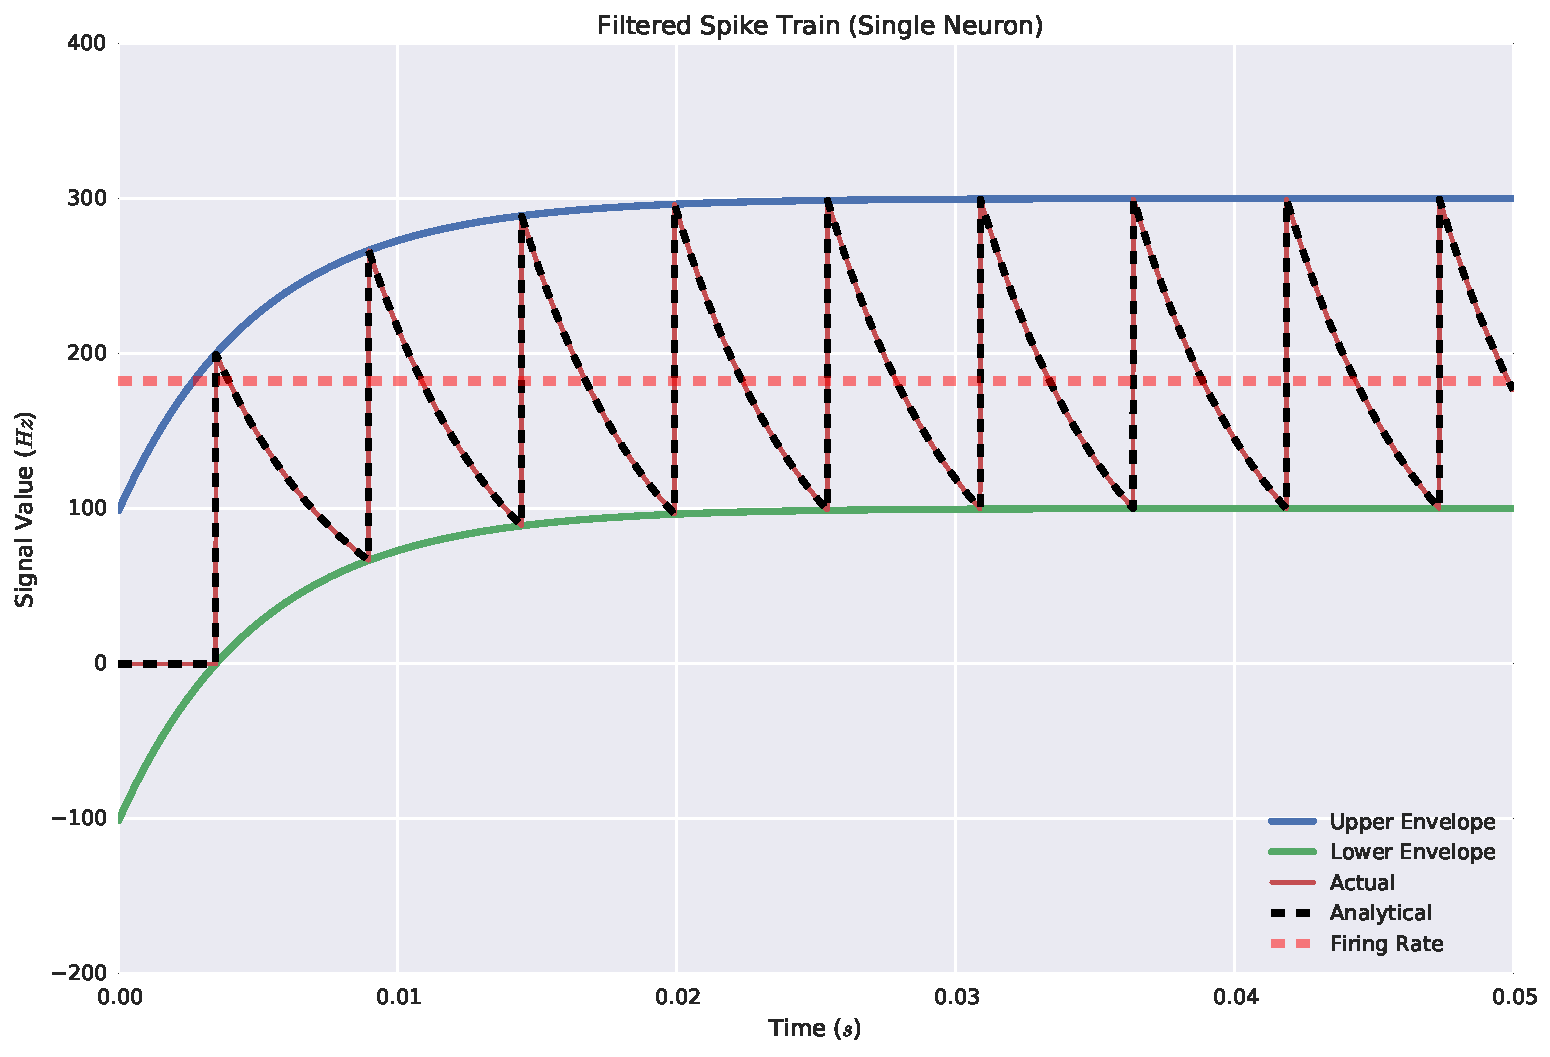
\includegraphics[width=1.0\textwidth]{slif-filtered}
\caption{\label{fig:slif-filtered} Filtered spike train under constant input ($\tau = 5\,$ms), matched by equation (\ref{eq:neuron}) and its bounds.}
\end{figure}

The boxed equation (\ref{eq:neuron}) perfectly characterizes the neuron's filtered spike train under the given assumptions. In addition, the lower/upper bounds of $\Delta_i(t; s_i)$ give the upper- and lower-envelopes, respectively:
\begin{equation*}
\frac{r_i - r_i^{a_i(t - s_i) + 1}}{\tau(1 - r_i)} < \tilde{a}_i(t; s_i) \le \frac{1 - r_i^{a_i(t - s_i) + 1}}{\tau(1 - r_i)} .
\end{equation*}

We also remark that for the LIF case, $s_i$ can be easily determined from the neuron's initial state and its input current $J_i$:
\begin{align*}
v_i(t) &= v_i(0) + (J_i - v_i(0))(1 - e^{-t/\tau_{RC}}) \\
\implies \quad s_i &= -\tau_{RC} \ln \frac{J_i - 1}{J_i}
\end{align*}
where $\tau_{RC}$ is the neuron's membrane time-constant. See \href{https://github.com/nengo/nengo/pull/975}{PR \#975} for details.

The analysis from \S\ref{sec:lowpass} can be used to obtain the precise form of the decoded estimate $\V{\tilde{x}}(t)$ at the population level. However, this depends on the initial spikes $s_i$, and so $\V{\tilde{x}}(t)$ can vary wildly depending on the initial state of all neurons.

For instance, if all neurons are initially at rest, then the estimate is most certainly zero until the fastest neuron fires. More critically, if all neurons have the same firing rate, but their initial spikes are not evenly distributed, then the error at the population level will be the addition of all their envelopes (as in the aside from the end of \S\ref{sec:integrator}).

For this work, we essentially assume that we have no control over the initial state of the system. That is, we suppose that the state of each neuron at $t = 0$ is independent and ``random'' (i.e., the previous input could have switched at any time). To be precise, we interpret $s_i$ as the realization of a random variable $S_i$ distributed by some chosen probability distribution.

Although the following analysis lends itself to the use of arbitrary distributions, some preliminary experimentation has shown that it is reasonable to assume:
\begin{equation}
\begin{gathered}
\label{eq:s}
S_i \sim U[0, 1/a_i] \\
\implies \quad f_{S_i}(s_i) = a_i \quad .  \quad \quad 
\end{gathered}
\end{equation}

This implies that the neuron is not initially biased to spike at any time in particular. In order for this to occur, we essentially require that the majority of neurons had non-zero activity in response to their prior input. In that situation, an arbitrary neuron could be at any point along its inter-spike interval, since it is not colluding with any other neurons.

In the NEF, this is typically a fair assumption, given that the tuning curves are broad (non-zero for half of the input space on average), and spike trains tend to be independent. However, for sparser encodings, or relatively large changes in input, the distribution becomes skewed towards $1 / a_i$. Similarly, if firing tends to be nearly synchronous, then the neurons will over-estimate whenever they spike together. This is noteworthy because this theory may give quantitative predictions regarding these trade-offs between encoding sparsity and firing rates, versus the desired accuracy and latency (see discussion).

Now, the analysis proceeds as follows. Fix $t$\footnote{This can be interpreted as the time that we decide to observe/measure the state of the system.} and then independently sample each $s_i$. This determines $\Delta_i(t; s_i)$ for each neuron, by the cyclic rotation $a_i s_i$ (modulo $1$) from (\ref{eq:delta}). We then define the random variable $\tilde{A}_i(t) := \tilde{a}_i(t; S_i)$, which we should understand as being distributed by ``mapping'' $S_i$ through the function $\tilde{a}_i$ for some chosen $t$. As an aside, for the special case of uniform $S_i$, the mapping $\tilde{a}_i$ actually corresponds to a cyclically shifted version of the inverse CDF of $\tilde{A}_i(t)$\footnote{This requires a subtle monotonicity argument. The CDF of $\tilde{A}_i$ can therefore be derived by inverting the unshifted $\tilde{a}_i$, but the result is not very nice to work with due to some discontinuities in its derivative.}.
%\begin{align}
%\label{eq:z}
%z_i(s_i; t) := \tilde{a}_i(t; s_i)
%\end{align}
%to view $Z_i(t)$ as a random variable that is obtained by ``mapping'' the distribution of $S_i$ through the function $\tilde{a}_i$ for some chosen $t$.  

Then the random variable $\V{\tilde{X}}(t) := \sum_i \V{d}_i \tilde{A}_i(t)$ is the decoded estimate obtained by forming a mixture of $\tilde{A}_i(t)$. The following subsections will analyze the expectation and variance of each $\tilde{A}_i(t)$ to determine the expected error and variability at time $t$.

\subsubsection{Expected Error}

By the law of the unconscious statistician (LOTUS) applied to $\tilde{A}_i(t)$:
\begin{align}
\label{eq:a_expectation}
E \left[ \tilde{A}_i(t) \right] &= \int_D \tilde{a}_i(t; s_i) f_{S_i}(s_i) \,ds_i, \quad \text{where $D$ is the domain of $S_i$} \nonumber\\
          &= \int_D \frac{r_i^{\Delta_i(t; s_i)} - r_i^{a_i(t - s_i) + 1}}{\tau(1 - r_i)} f_{S_i}(s_i) \,ds_i, \quad \text{by (\ref{eq:neuron})} \nonumber\\
          &= \frac{1}{\tau(1 - r_i)} \left( \int_0^{1} r_i^{\Delta_i(t; s_i)} \,d\Delta_i(t; s_i) - \int_0^{1/a_i} r_i^{a_i(t - s_i) + 1} (a_i) \,ds_i \right) \nonumber\\
          &= \frac{1}{\tau(1 - r_i)} \left( (-a_i \tau) e^{-\Delta_i(t; s_i)/a_i \tau} \bigg|_{\Delta_i(t; s_i) = 0}^{1} - (a_i \tau) r_i^{a_i(t - s_i) + 1} \bigg|_{s_i = 0}^{1/a_i} \right) \nonumber\\
          &= \frac{a_i}{(1 - r_i)} \left(  (1 - r_i) - (r_i^{a_i t} - r_i^{a_i t + 1})  \right) \nonumber\\
          &= a_i (1 - e^{-t/\tau}) .
\end{align}

Including the initial state of the synapse, $\V{x}_0$, the expected error at time $t$ is:
\begin{align}
\label{eq:expectation}
\implies \quad E\left[ \V{\hat{x}} - (\V{\tilde{X}}(t) + \V{x}_0 \, e^{-t/\tau}) \right] &= \sum_i \V{d}_i (a_i - E \left[ \tilde{A}_i(t) \right]) - \V{x}_0 \, e^{-t/\tau} \nonumber \\
&= \sum_i \V{d}_i a_i e^{-t/\tau} - \V{x}_0 \, e^{-t/\tau} \nonumber  \\
\Aboxed{ &\,= (\V{\hat{x}} - \V{x}_0) e^{-t/\tau} . }
\end{align}

\begin{figure}[h!]
\centering
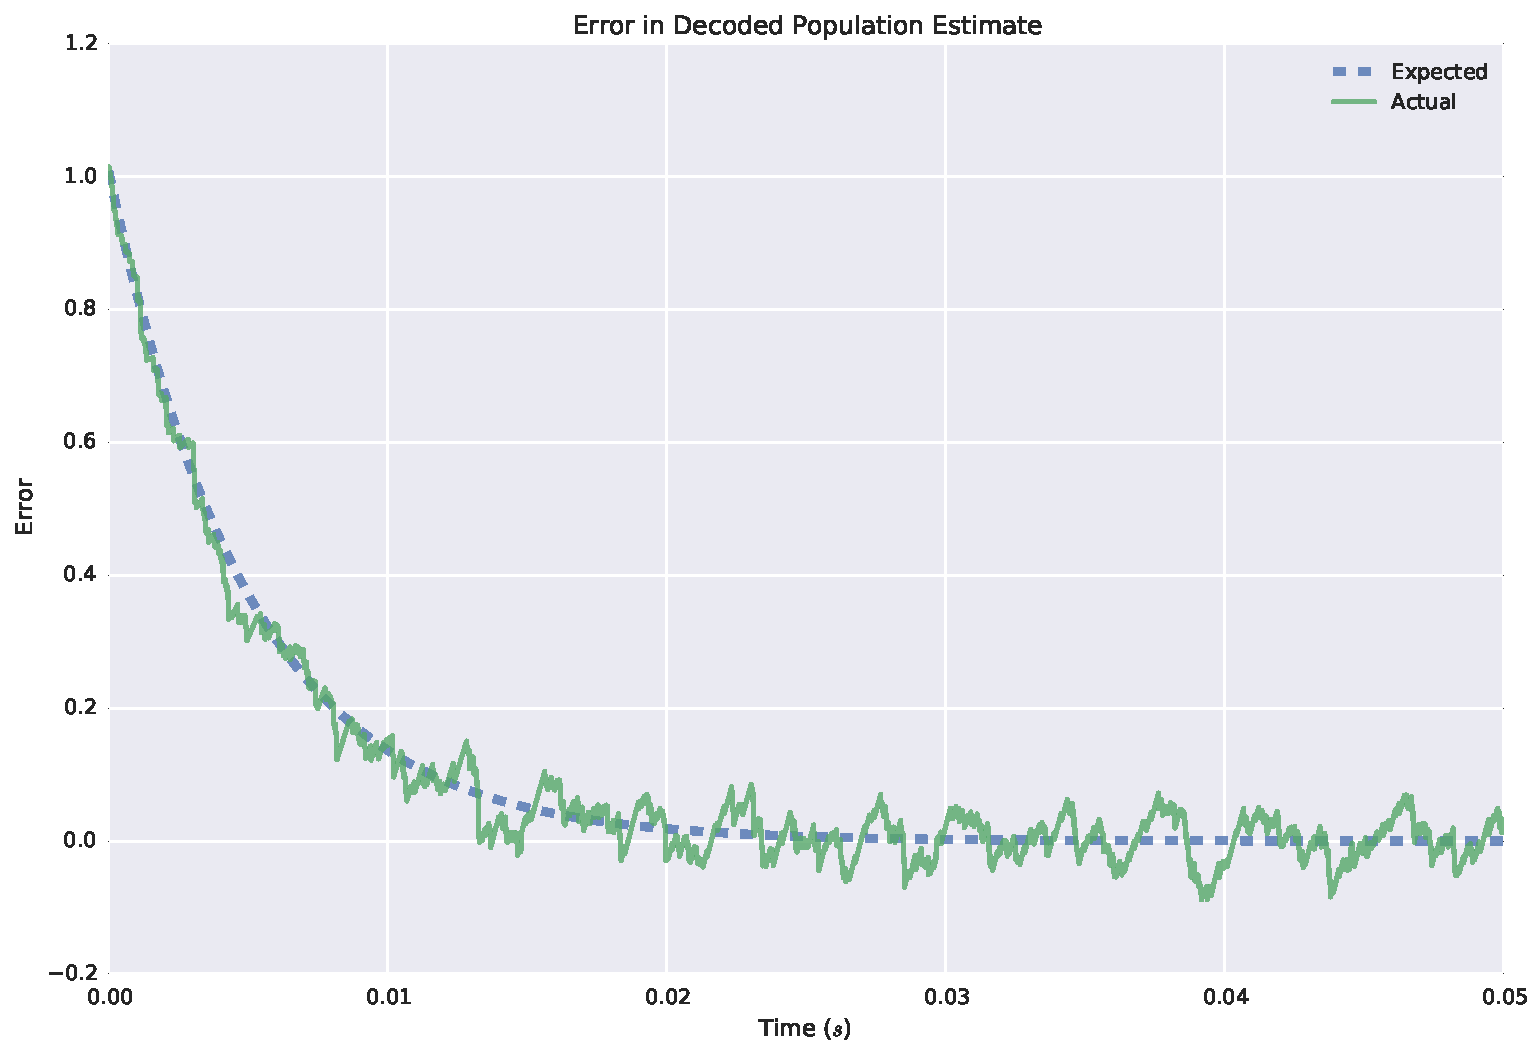
\includegraphics[width=1.0\textwidth]{slif-error}
\caption{\label{fig:slif-error} Error from filtered and decoded estimate using a population of $100$ neurons ($\tau = 5$\,ms, $\V{x}_0 = -0.2$, and $\V{\hat{x}} \approx \V{x}_0 + 1$). The expectation from (\ref{eq:expectation}) is given by the dashed line.}
\end{figure}

On one hand this is what we should intuitively expect, since we are essentially filtering an error signal using the same lowpass with an initial state given by the initial error. But it should also be surprising that this result holds independently of the width ($1 / a_i$) of each inter-spike interval, while we have only assumed the initial spikes are uniformly distributed across these intervals (in fact the independence assumption has not been used). If all neurons were initially at rest, then this result clearly no longer holds (consider $0 < t < \min_i 1/a_i$).

This assures us that we can set $\tau \rightarrow 0$ to minimize latency without hurting the expected error. However, as we will soon see, this comes at the cost of increasing the variability of the estimate.

\subsubsection{Variance in Error}

To compute $Var \left[ \tilde{A}_i(t) \right] = E \left[ \tilde{A}_i(t)^2 \right] - E \left[ \tilde{A}_i(t) \right]^2$ we rewrite the second moment:
\begin{align*}
E \left[ \tilde{A}_i(t)^2 \right] &= E \left[ \left( \frac{r_i^{\Delta_i(t; S_i)} - r_i^{a_i(t - S_i) + 1}}{\tau(1 - r_i)} \right)^2 \right] \\
&= \left( \frac{1}{\tau(1 - r_i)} \right)^2 \left( E \left[ (r_i^{\Delta_i(t; S_i)})^2 \right ] - 2 E \left[ r_i^{\Delta_i(t; S_i) + a_i(t - S_i) + 1} \right] + E \left[ (r_i^{a_i(t - S_i) + 1})^2 \right] \right)
\end{align*}
and then separately determine each expectation.

The PDFs of $r_i^{\Delta_i(t; S_i)}$ and $r_i^{a_i(t - S_i) + 1}$ are both $a_i \tau / x$ over their respective domains. This can be seen directly:
\begin{align*}
\frac{\partial}{\partial x} Pr \left[ r_i^{\Delta_i(t; S_i)} \le x \right] &= \frac{\partial}{\partial x} Pr \left[ \Delta_i(t; S_i) \le -a_i \tau \ln x \right] \\
&= \frac{\partial}{\partial x} (1 - (-a_i \tau \ln x)) \\
&= a_i \tau / x .
\end{align*}
and the proof for $r_i^{a_i(t - S_i) + 1}$ is analogous. We remark that these two facts can be used to give a slightly different derivation for (\ref{eq:a_expectation}). 

Applying LOTUS to each of these random variables gives:
\begin{align*}
E \left[ (r_i^{\Delta_i(t; S_i)})^2 \right ] &= \int_{r_i}^1 \frac{a_i \tau}{x} x^2 \,dx = \frac{a_i \tau x^2}{2} \bigg|_{x = r_i}^1 = \frac{a_i \tau (1 - r_i^2)}{2} \\
E \left[ (r_i^{a_i(t - S_i) + 1})^2 \right] &= \int_{r_i^{a_i t + 1}}^{r_i^{a_i t}} \frac{a_i \tau}{x} x^2 \,dx = \frac{a_i \tau x^2}{2} \bigg|_{x = r_i^{a_i t + 1}}^{r_i^{a_i t}} = \frac{a_i \tau (1 - r_i^2) r_i^{2 a_i t}}{2} .
\end{align*}

To compute the remaining expectation, we need to get some further understanding of $\Delta_i(t; S_i) = (a_i(t - s_i) + 1) - \floor{a_i(t - s_i) + 1}$. Define $K_i(t) := \floor{a_i t}$ as the current interval independent of $s_i$. %Then the $i^{th}$ neuron has spiked $K_i(t - s_i) + 1 = \floor{a_i(t - s_i) + 1}$ times at time $t$. More importantly, 
The point \mbox{$s_i = t - K_i(t)/a_i \equiv t \ (\text{mod}\ 1/a_i)$} gives the discontinuity in $\Delta_i(t; s_i)$ with respect to $s_i$, because that is when the spike becomes aligned with $t$ in the current interval. Namely, if $0 \le s_i \le t - K_i(t)/a_i$, then $\floor{a_i(t - s_i) + 1} = \floor{K_i(t) + 1} = K_i(t) + 1$. Likewise, if $t - K_i(t)/a_i < s_i \le 1/a_i$, then $\floor{a_i(t - s_i) + 1} = K_i(t)$\footnote{If this is confusing, recall that we are fixing $t$ and then sweeping $s_i$ from $0$ to $1 / a_i$.}. Then use LOTUS once more, along with the above fact to split up the integral.
\begin{align*}
E \left[ r_i^{\Delta_i(t; S_i) + a_i(t - S_i) + 1} \right] &= \int_0^{1/a_i} r_i^{2(a_i(t - s_i) + 1) - \floor{a_i(t - s_i) + 1}} (a_i) \, ds_i \\
&= a_i \left( \int_0^{t - K_i(t)/a_i} r_i ^ {(2a_i t - K_i(t) + 1) - (2a_i s_i)} \, ds_i + \int_{t - K_i(t)/a_i}^{1/a_i} r_i^{(2a_i t - K_i(t) + 2) - (2a_i s_i)} \, ds_i \right) \\
&= a_i r_i^{2a_i t - K_i(t) + 1} \tau / 2 \left( e^{2s_i / \tau} \bigg|_{s_i=0}^{t - K_i(t)/a_i} + r_i e^{2s_i / \tau} \bigg|_{s_i=t - K_i(t)/a_i}^{1/a_i} \right) \\
&= a_i r_i^{2a_i t - K_i(t) + 1} \tau / 2 \left( r_i^{-2 a_i(t - K_i(t)/a_i)} - 1 + r_i^{-1} - r_i^{-2a_i(t - K_i(t)/a_i) + 1} \right) \\
&= a_i \tau (1 - r_i)(r^{K_i(t) + 1} + r_i^{2a_i t - K_i(t)}) / 2
\end{align*}

Plugging these all in then gives:
\begin{align*}
Var \left[ \tilde{A}_i(t) \right] = \, \Aboxed{ a_i \left( \frac{(1 - r_i^2)(1 + r_i^{2a_i t})}{2\tau(1 - r_i)^2} - \frac{\left( r_i^{K_i(t) + 1} + r_i^{2a_i t - K_i(t)} \right)}{\tau(1 - r_i)} - a_i(1 - r_i^{a_i t})^2 \right) }
\end{align*}

\begin{align}
\label{eq:variance}
\implies \quad Var\left[ \V{\hat{x}} - (\V{\tilde{X}}(t) + \V{x}_0 \, e^{-t/\tau}) \right] = Var\left[ \V{\tilde{X}}(t) \right]
= \sum_i \V{d}_i^2 \, Var\left[ \tilde{A}_i(t) \right] .
\end{align}

\begin{figure}[h!]
\centering
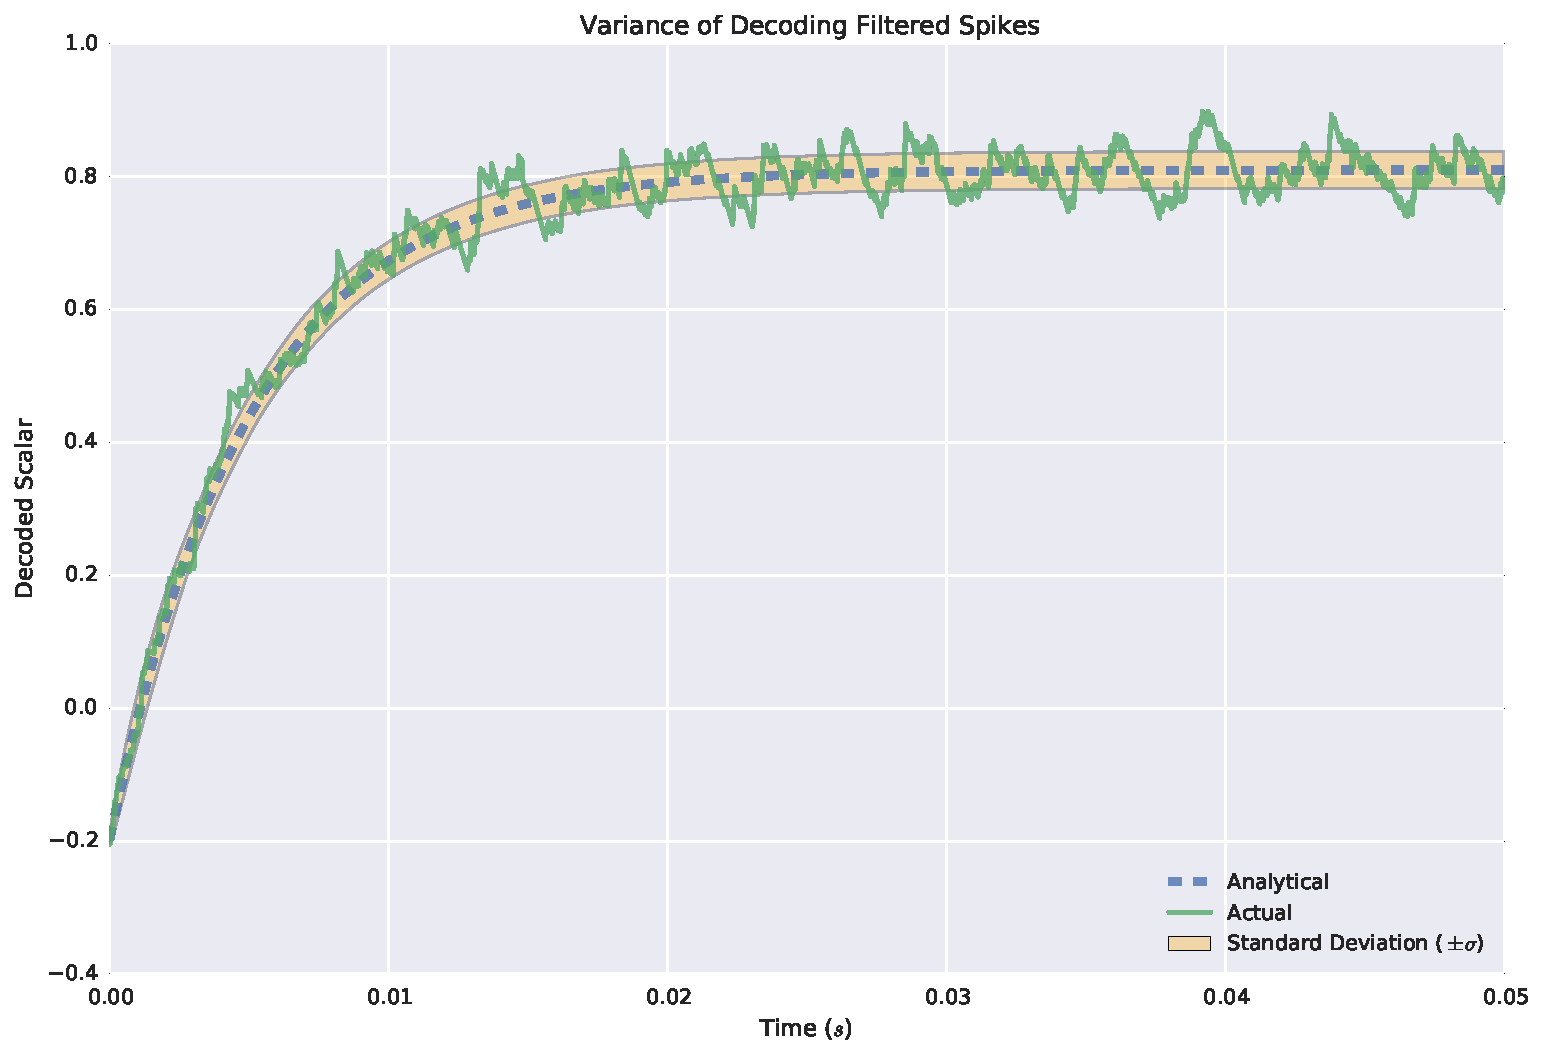
\includegraphics[width=1.0\textwidth]{slif-variance}
\caption{\label{fig:slif-variance} Filtered and decoded estimate using the same network as Fig.~\ref{fig:slif-error}. The variance is highlighted by one standard deviation from the mean.}
\end{figure}

\subsubsection{Validity of Uniform Assumption}

\begin{figure}[h!]
\centering
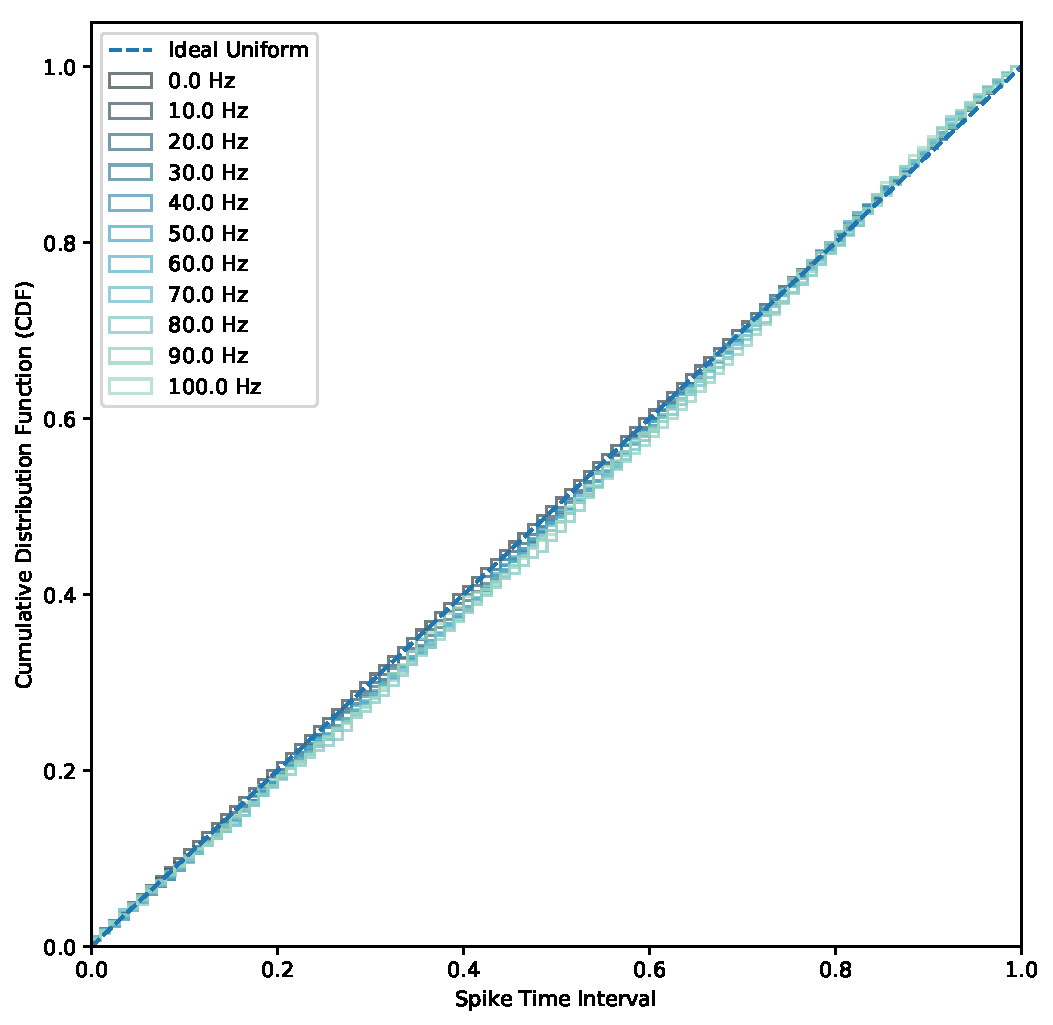
\includegraphics[width=1.0\textwidth]{spike-time-intervals}
\caption{\label{fig:spike-time-intervals} Empirical distribution of ISI positions---$s_i$ normalized by the instaneous rate $a_i$---for sinusoid stimuli of varying frequencies.
  The ideal distribution (dashed) is uniform $[0, 1]$. In the ideal case, the spiking LIF model is equal to its non-spiking counterpart in the sense of expectation.
}
\end{figure}

The previous analysis relies on the assumption that each neuron is ``uniformly ready to spike''.
To validate this assumption from equation (\ref{eq:s}) that $S_i \sim U[0, 1/a_i]$, we empirically sampled this distribution for sinusoidal test stimuli of varying frequencies (Fig.~\ref{fig:spike-time-intervals}).
We define the \emph{ISI position} as $s_i \times a_i$. This is the realization of a random variable, in the range $[0, 1]$.
Intuitively, this can be interpreted as the percent time remaining within the idealized inter-spike interval, given the current voltage of the neuron and its ideal spike rate.
A value of $0$ implies the neuron is currently spiking and $1$ implies the neuron just spiked.
This quantity is calculated by solving the LIF ODE and rearranging to obtain:
\begin{equation}
\left(\tau_\text{RC} \log\left(1 + \frac{1 - v_i}{J_i - 1}\right) + r_i \right) a_i \text{,}
\end{equation}
where $0 \le r_i \le \tau_\text{ref}$ is the time remaining in the refractory period.

As shown in Fig.~\ref{fig:spike-time-intervals}, the default LIF model ($\tau_\text{RC} = 20$\,ms, $\tau_\text{ref} = 2$\,ms, and tuning curves uniformly distributed to achieve maximum firing rates of $200-400$\,Hz) closely follows the ideal uniform distribution for input frequencies up to $100$\,Hz. For $0$\,Hz (constant) inputs, the two distributions are the same (Kolmogorov-Smirnov statistic=0.0002, $p$-value=0.999999999999999)\footnote{When the sample comes from the same distribution, its Kolmogorov-Smirnov statistic approaches $0$ with probability $1$ as the number of samples goes to infinity.}.
This acts as a sanity check on the numerics of our spiking LIF implementation\TODO{cite Nengo LIF improvements}, as we should expect that a constant input causes each neuron to spend an equal amount of time at each position within its ideal ISI.
For changing inputs, however, the uniform assumption immediately breaks down ($p$-value $< \numprint{1e-67}$), but non-catastrophically, as the Kolmogorov-Smirnov statistic (i.e., the supremum between the empirical and ideal CDFs) remains bounded above by $0.0335$.

Taken together, this means that any approximation error arising from the substitution of spiking LIF for non-spiking LIF models must arise from two sources: (1) the variability in equation \ref{eq:variance}, which is a function of $\tau$, the number of neurons, and the magnitude of the decoders, and (2) a systematic bias (Fig.~\ref{fig:spike-time-intervals}) resulting from the ISI positions being non-uniform with respect to the input stimuli.
In summary, this provides a theoretical framework for understanding the differences between spiking and non-spiking neuron models in the context of some desired PSC.
This also provides some theoretical justification for using spiking LIF models following an offline optimization using static tuning curves -- a procedure that the NEF and Nengo use regularly.
Lastly, this suggests criteria for optimizing the information-processing capabilities of spiking neurons in the context of high-frequency signals, as done in section~\ref{sec:poisson-spiking}.

\TODO{Comment on dimensional analysis for speeding up / slowing down timescales}

\subsection{Efficiency in Time and Space}

Low-rank factorization is optimal in space and time assuming linear weights (there is no advantage to factoring it any further by linearity).

\subsection{Turing-Completeness}


\subsection{Robustness}

Robustness to noise.

Also Conjecture: Den\`eve doesn't work in chaotic settings. NEF does (voltage vector is chaotic). NEF and FORCE are doing the same thing -- the latter just adds extra chaos in because Reservoir Computing.



Expose the general ideas about mapping NEF networks onto neuromorphic hardware, and what makes it better than other frameworks.


\subsection{Extensibility}

Section~\ref{chapt:nef-extensions}.

\chapter{Methodology}
\label{chapt:methodology}

This chapter is devoted to a brief overview of our methods, namely the software tools that we use, and our approaches to modelling useful computations as dynamical systems.
Additional details are the focus of later chapters.

\section{Software}
\label{sec:software}

The simulations in this thesis make extensive use of the following Python software packages (versions listed when important):
\begin{itemize}
\item Nengo 2.8.0~\citep{bekolay2014}; to construct and simulate NEF models on the CPU, which depends on NumPy for its algebraic routines,
\item Nengo-Loihi 0.5.0~\citep{blouw2018a, nengoloihi}; to compile Nengo models onto the Loihi emulator and hardware (courtesy of ABR),
\item Nengo-Brainstorm~\citep[pre-release;][courtesy of Terry Stewart]{neckar2018optimizing, braindrop2019}; to compile Nengo models onto Braindrop, which depends on PyStorm (courtesy of the Boahen Lab),
\item HyperOpt 0.0.2~\citep{bergstra2015hyperopt}; to optimize the hyperparameters associated with RC networks,
\item Keras 2.2.4~\citep{gulli2017deep}; to train LSTMs and some custom RNNs,
\item TensorFlow 1.12.0~\citep{abadi2016tensorflow}; as a backend for Keras,
\item Seaborn~\citep{michael_waskom_2015_19108}; to generate figures, which depends on Matplotlib and Pandas for plotting and formatting data, respectively.
\end{itemize}
We do not take credit for any of the above software.
However, we have created the Python package, NengoLib 0.5.0~\citep[][patent~pending]{dynamicspatent, nengolib}, open-sourced on GitHub, to make the contributions of this thesis publicly available.
% which also depends on SciPy for many routines ported from MatLab
Code, \LaTeX{}, and instructions for reproducing figures, are located at: \url{https://github.com/arvoelke/phd/}.
Unless stated otherwise, all simulations use a time-step of $\dt{} = 1$\,ms, and assume the input signal is held constant across each time-step, also known as the ``zero-order hold''~(ZOH) assumption.
Experiments that implement the methods of \citet{boerlin2013predictive} in Nengo are currently unpublished (provided by Dan Rasmussen).

%\subsection{NengoLib}
%\label{sec:nengolib}

NengoLib includes the core code for most of the extensions discussed in chapter~\ref{chapt:nef-extensions} and the networks discussed in chapter~\ref{chapt:delays}.
It has been used by publications including
\citet{knight2016}, \citet{voelker2016a}, \citet{voelker2017iscas}, \citet{voelker2017neuromorphic}, and \citet{voelker2018}.
In addition, we use it to construct RC, FORCE, full-FORCE, and Nengo networks---each in spiking and non-spiking mode, and in an analogous manner to one another---in order to facilitate meaningful comparisons between these architectures.
A core feature of this software is a toolkit for constructing and analyzing linear time-invariant systems, in a number of representations (state-space, transfer function, zero-pole-gain), while being compatible with the synapses of Nengo.
This unifies the language used to build, describe, and analyze LTI networks, synapses, and sub-threshold neural dynamics.
We now summarize some additional features of this software that are used throughout.

\subsubsection{State-space realizations}

This section has been adapted from \citet[][appendix~A.3]{voelker2018}.
The state-space model (equation~\ref{eq:lti}) is \emph{not} a unique description of the input-output behaviour of an LTI system.
In general, one may consider any invertible matrix $T$ with the same shape as $A$, and observe that the state-space model $(TAT^{-1}\text{,}\, TB\text{,}\, CT^{-1}\text{,}\, D)$ has the same transfer function as $(A\text{,}\, B\text{,}\, C\text{,}\, D)$.
Thus, the state-space model is only unique up to a change of basis.
However, in the NEF, the basis $T$ may be ``absorbed'' into the representation of $\V{x}(t)$ by using the encoders $ET$ in Principle~1, which, in turn, results in the decoders $D^\V{f} \transpose{\left(T^{-1}\right)}$ from Principle~2.
In other words, considering an alternative state-space model is equivalent to considering a change of basis for the representation.
Nevertheless, in practice, when aiming to accurately represent $\V{x}(t)$ using few neurons, it is important to balance the relative range of values within each dimension, such that a typical trajectory for $\V{x}(t)$ stays within the space represented by the distribution of encoders, consistent with the samples of $S$ (see equation~\ref{eq:decoder_solution}), and the dynamic range of each neuron.

For this, there is a feature to \emph{balance} the range of values by numerically computing the $T$ that results in a ``balanced realization'' of $(A\text{,}\, B\text{,}\, C\text{,}\, D)$~\citep{laub1987computation, perevapproximation}.
We then set the encoders to be unit-length and axis-aligned, and optimize each dimension independently by using the methods from section~\ref{sec:principle2}.
There is also the support to normalize each dimension by a diagonal transformation $T$ with the $i^{\text{th}}$ diagonal equaling $\max_t \left| x_i(t) \right|^{-1}$ where $x_i(t)$ is obtained by simulating the ideal system directly on a randomly sampled input.
Finally, NengoLib supports a diagonal transformation $T$ with the $i^{\text{th}}$ diagonal corresponding to the reciprocal of two times the sum of the Hankel singular values~\citep{glover1987bounds} of the subsystem corresponding to $x_i(t)$.
This has the effect of bounding the absolute value of each dimension above by $1$ in the worst case~\citep{khaisongkram2007computing}.

In general, we find that each of the above methods to normalize state-space models typically improves the robustness of our networks across a wide range of parameters, but one is never strictly better than all others in every situation.

% Likewise, any change of basis in the state-space model of $F^H$ does not impact the dynamics of $F^H(H(s)^{-1})$
% But there is really no reason to do that as far as I can tell.
%It is worth noting that the mappings from section~\ref{sec:extensions}---with the exception of equations~\ref{eq:lambert-delay} and~\ref{eq:general-linear-approx}---do not alter the representation of $\V{x}(t)$.
%Disregarding these exceptions, the same choice of basis is conveniently carried over to the implemented network.
%Yet, it is also the case that the dynamics of the system mapped by equation~\ref{eq:general-linear-approx} do not depend on the chosen state-space model.
%This fact is proven implicitly in the following appendix, by characterizing the dynamics in terms of $F(s)$ and $H(s)$ alone.

%\url{https://arvoelke.github.io/nengolib-docs/master/notebooks/research/geometric\_decoders.html}

\subsubsection{Random sampling}

Many common routines in Nengo employ the use of high-dimensional random sampling~\citep{voelker2017, gosmann2018}, in particular the uniform sampling of encoders $\V{e}_i$ from the surface of the hypersphere, and the uniform sampling of evaluation points from $S$ (typically the interior of the hyperball).

Considering the NEF's optimization problem from equation~\ref{eq:decoder_solution},
Monte Carlo~(MC) sampling $S$ introduces $\bigoh{ m^{-\frac{1}{2}} }$ error into the integral, where $m$ is the number of samples, but this can be improved to $\widetilde{\mathcal{O}} \left( m^{-1} \right)$---effectively squaring $m$---by the use of quasi-Monte Carlo methods~\citep{fang1994, knight2016}.
For this, NengoLib overloads Nengo's default versions of these distributions, with its own method of uniformly scattering the samples using quasi-MC sampling.
Specifically, we take a scattered sample from the hypercube, and then apply the inverse transform method with a spherical coordinate transform~\citep{fang1994} to map samples onto either the hyperball or hypersphere.
This supports the use of any number of quasi-MC methods for sampling from the cube, although we have implemented the most promising ones: Sobol sequence and $R_2$~\citep{Sobol1967, quasimc}.

We find that quasi-MC sampling the encoders also improves the representation at low numbers of neurons on average, by ensuring a better tiling or coverage of the encoded space.
For efficient coding in higher dimensions, methods of randomly sampling points from the Leech lattice---a 24-dimensional Lattice built from \numprint{196560} unit-length vectors, with beautiful mathematical properties regarding their similarity in relation to efficient sphere-packing and error-correction codes~\citep{Conway1999}---used by \citet{knight2016} are also available in NengoLib.

% \subsubsection{Vector Oja Learning Rule}

\section{Dynamics as a language}
\label{sec:dynamics-language}

As discussed in section~\ref{sec:nef-turing}, dynamical systems represent a complete (i.e.,~universal) model of computation.
But how are useful high-level computations embedded into such systems?
To this end, we are interested in developing a language for describing useful algorithms within the dynamical modelling framework of the NEF, and libraries for combining these models within Nengo.

Early work by \citet{eliasmith2003a} has shown that many important neurobiological systems, such as the nuclei involved in horizontal eye control, may be modelled as an integrator.
That is, some velocity signal, indicating a desired direction, is represented by one population and then integrated by another.
Such systems are describable as a one-dimensional linear time-invariant system (see equation~\ref{eq:lti}), such as the one demonstrated in section~\ref{sec:chaos} using ten spiking neurons. 
When extended to higher dimensions, this same system is capable of storing multiple items in series, and has consequently been applied to build sophisticated models of working memory~\citep{singh2004, choo2010}.

Oscillatory dynamics (e.g.,~relaxation oscillators), such as those modelled in \citet{eliasmith2000b} have utility in generating rhythmic activity to support various computations.
For example, theta oscillations in the range of $4$--$12$\,Hz, through a phenomenon known as phase precession, have been shown to support the encoding of spatial information using Nengo~\citep{o1993phase, orchard2013does}.
Likewise, a bank of oscillators can be used to facilitate motion processing in the early visual system~\citep{huzook2012}. 

Attractor networks describe a much broader class of nonlinear dynamical systems that capture many important phenomena observed in neurobiological systems~\citep{amit1989modeling, eliasmith2005b}.
When oscillations, integrators, and point attractors, are all combined, networks may generate complex trajectories through space~\citep{ijspeert2013dynamical, dewolf2017}.
By arranging all of these building blocks in an engineered fashion, together with feed-forward synaptic dynamics coupling various modules, complex systems such as Spaun may carry out end-to-end cognitive tasks and even learn to follow general sets of instructions~\citep{eliasmith2012, choo2018}.
The role of chapter~\ref{chapt:delays} is to unveil another class of dynamical systems for continuous nonlinear memory, that connects with ``time cell'' data from the neuroscience literature, and naturally fits into this framework.
But first, we describe a few concrete examples to help illustrate the universality of dynamical descriptions of computation, in a number of distinct contexts.

\subsection{Winner-take-all}

Winner-take-all~(WTA) circuits essentially engineer a ``$\max$'' function that pools across \emph{spatial} dimensions.
These systems may be described in state-space using nonlinear differential equations, that compete with one another in order to resolve the correct solution over time, as in an attractor network~\citep{usher2001time, gosmann2017a}.
Here, we are interested in a very different kind of WTA circuit that must compute its $\max$ across temporal dimensions.
We call this circuit a ``peak detector''.\footnote{%
This problem was proposed by Jan Gosmann (unpublished).}
Specifically, we suppose the input vector, $\V{u} \in \mathbb{R}^m$, is supplied online, one dimension at a time, such that:
$$\V{u}[k] = \transpose{\left( u[k] \text{,}\, u[k-1] \text{,}\, \ldots \text{,}\, u[k-m] \right)}$$
for some (possibly infinite) number of samples, $m \ge 1$.
In this context, determining the maximum of $\V{u}[k]$ is equivalent to the task of tracking the peak of the past history of the discrete-time signal, $u[k]$ (see Figure~\ref{fig:wta-peak-detector}), at a sampling interval of $\dt{}$.
In other words, the problem of tracking the maximum across time, is equivalent to a WTA mechanism where the input dimensions are provided sequentially, as opposed to being provided all at the same moment in time (as is usually the case).

\fig{wta-peak-detector}{0.5}{Peak detector as a dynamical system.}{
  An ideal ``peak detector'' implemented as a discrete-time dynamical system.
  This is equivalent to performing a winner-take-all across data provided sequentially.
}

In the limit of $\dt{} \rightarrow 0$, the desired continuous-time dynamical system is:
\begin{equation}
\label{eq:peak-detector-continuous}
\dot{x}(t) = f(x(t), u(t)), \quad f(x, u) = \theta^{-1} \left[u - x \right]_+
\end{equation}
where $\left[ \cdot \right]_+$ denotes positive half-wave rectification. $\theta > 0$ is a time-constant that determines how quickly the state should adjust to the positive difference. Note that in a purely continuous-time system, assuming no noise, $\theta$ can be made arbitrarily small, in order to track the peak arbitrary quickly. 
However, since we have a discrete sampling time, our desired dynamical system is:
\begin{equation}
\label{eq:peak-detector-discrete}
x[k + 1] = \bar{f}(x[k], u[k]), \quad \bar{f}(x, u) = \bar{\theta}^{-1} \left[u - x \right]_+ + x
\end{equation}
where $\bar{\theta} > 0 $ is a (dimensionless) discrete time-constant.
Equation~\ref{eq:peak-detector-discrete} is related to equation~\ref{eq:peak-detector-continuous} by $\bar{\theta} = \theta \left( \dt{} \right)^{-1}$, assuming Euler integration.
Note that $\bar{\theta} = 1$ will give a perfect peak detector, assuming no noise.

In Figure~\ref{fig:wta-peak-detector}, we implement a peak detector by using Nengo directly as a dynamical systems simulator. This does not use any neurons, but rather digitally implements equation~\ref{eq:peak-detector-discrete} with $\bar{\theta} = 1$ by coupling each variable in the correct way:
\begin{python}
with nengo.Network() as model:
    u = nengo.Node(stim)  # stim defines the test input signal
    peak = nengo.Ensemble(1, dimensions=2, neuron_type=nengo.Direct())
    nengo.Connection(u, peak[1], synapse=None)
    function = lambda x: (x[1] - x[0]).clip(min=0) + x[0]
    nengo.Connection(peak, peak[0], synapse=~z, function=function)
\end{python}
We remark that $\textasciitilde z$ is a dynamical primitive in NengoLib that implements a single time-step delay, in correspondence with the $\mathcal{Z}$-transform in signal processing.
This illustrates the utility of discrete-time dynamical systems, the flexibility of this framework for describing useful computations, and the versatility of Nengo as a programming tool for simulating such systems.
Both continuous-time and discrete-time versions of this system may be implemented using spiking neurons as well (not shown).
In chapter~\ref{chapt:nef-extensions} we will address the implementation of such systems---with both discrete- and continuous-time dynamics---using populations of spiking neurons in analog and digital hardware.

\subsection{Unsupervised learning}
\label{sec:unsupervised}

This section has been adapted from \citet{voelker2014a}, and discusses the dynamics of an unsupervised learning rule used by \citet{voelker2014controlling}, \citet{trujillo2014a}, and \citet{aubin2016a}.
This has been implemented on SpiNNaker~\citep{knight2016}, and is discussed in some detail by \citet{aubin2018}.
Here we expose the dynamics of this learning rule, while highlighting its function for sparsifying across space in large-scale models.

Associative memories have been an active area of research over the last forty years~\citep{willshaw1969nonholographic, kohonen1972, hopfield1982} because they form a central component of many cognitive architectures~\citep{Pollack1988, Anderson1998}.
We focus specifically on associative memories that store associations between arbitrary pairs of neural states.
When a noisy version of an input state vector is presented to the network, it must output a ``clean'' version of the associated state vector.
\citet{stewart2011biologically} has built such a memory network, possessing a number of desirable properties including: high accuracy, a fast, feed-forward recall process, and efficient scaling, requiring a number of neurons linear in the number of stored associations.
 These memories have played a central role in several cognitive models including Spaun, as well a proposal for human-scale, biologically-plausible knowledge representation~\citep{crawford2015}.
However, these memories are constructed using an offline optimization method that is not biologically-plausible.

We describe a method for building large-scale networks for online learning of associations using spiking neurons.
Connection weights can be arrived at through a biologically-plausible, online learning process featuring a novel synaptic learning rule inspired in part by the well-known Oja learning rule~\citep{oja1989neural}.
We call this rule the \emph{voja} learning rule (for ``vector Oja'').
Although the network itself is feed-forward, the dynamics that carry out the important computations are embedded within the learning rules that modify its synaptic weights online.
We now describe the learning rule.

Given a learning rate $\eta$, an input vector $\V{x}$ encoded by the activity of the input layer, the filtered activity $a(t)$ of  neurons in the middle layer, and the matrix $E$ whose rows are the ``preferred direction'' vectors of the middle layer neurons, we modify the preferred direction vectors of the middle layer neurons according to the dynamical system:
\begin{align} \label{voja}
    \Delta{E} = \eta \left( a(t) \transpose{\V{x}} - a(t)E \right) = \eta a(t) \left( \begin{pmatrix} \transpose{\V{x}} \\ \vdots \\ \transpose{\V{x}} \end{pmatrix} - E \right) \text{.}
\end{align}
To understand the effect of this rule over time, we set $\Delta{E_i} = 0$ and solve for the fixed point.
This gives $a_i(t) \V{x} = a_i(t) \V{e}_i$, and thus, for a particular $\V{x}$, convergence is characterized by:
\begin{align} \label{stability}
    [\Delta{\V{e}_i} = 0]  \iff  [a_i(t) > 0  \implies  \V{e}_i = \V{x}] \text{.}
\end{align}
In plain words, the encoding vectors of the neurons that become active will, over time, become more active and store the input within its encoder.
The effect of this rule is to self-organize a sparse representation, such that a subset of neurons fire only when $\V{x}$, or a similar enough (i.e.,~noisy) version of it, is presented (see Figures~\ref{fig:voja-spinnaker} and~\ref{fig:voja-encoders}).
The preferred direction vectors of each neuron are embedded within the synaptic weights projecting from the previous layer.
Thus, this can be realized as a local learning rule by multiplying the decoders through and expressing the update as its weight with the $j^\text{th}$ presynaptic neuron~\citep{knight2016}:
\begin{align}
  \label{eq:voja-weights}
  \Delta \omega_{ij} = \Delta \V{e}_i \cdot \V{d}_j = \eta \, a_i (\V{d}_j \cdot \V{x} - \omega_{ij}) \text{.}
\end{align}
In effect, this rule achieves some useful computation---the unsupervised learning of inputs---by implementing a dynamical system within the state of each synapse.
The networks of \citet{knight2016, aubin2016a} learn to associate each input vector with a distinct output vector, by combining this rule with a supervised learning rule discussed below.

\begin{figure}
    \centering
  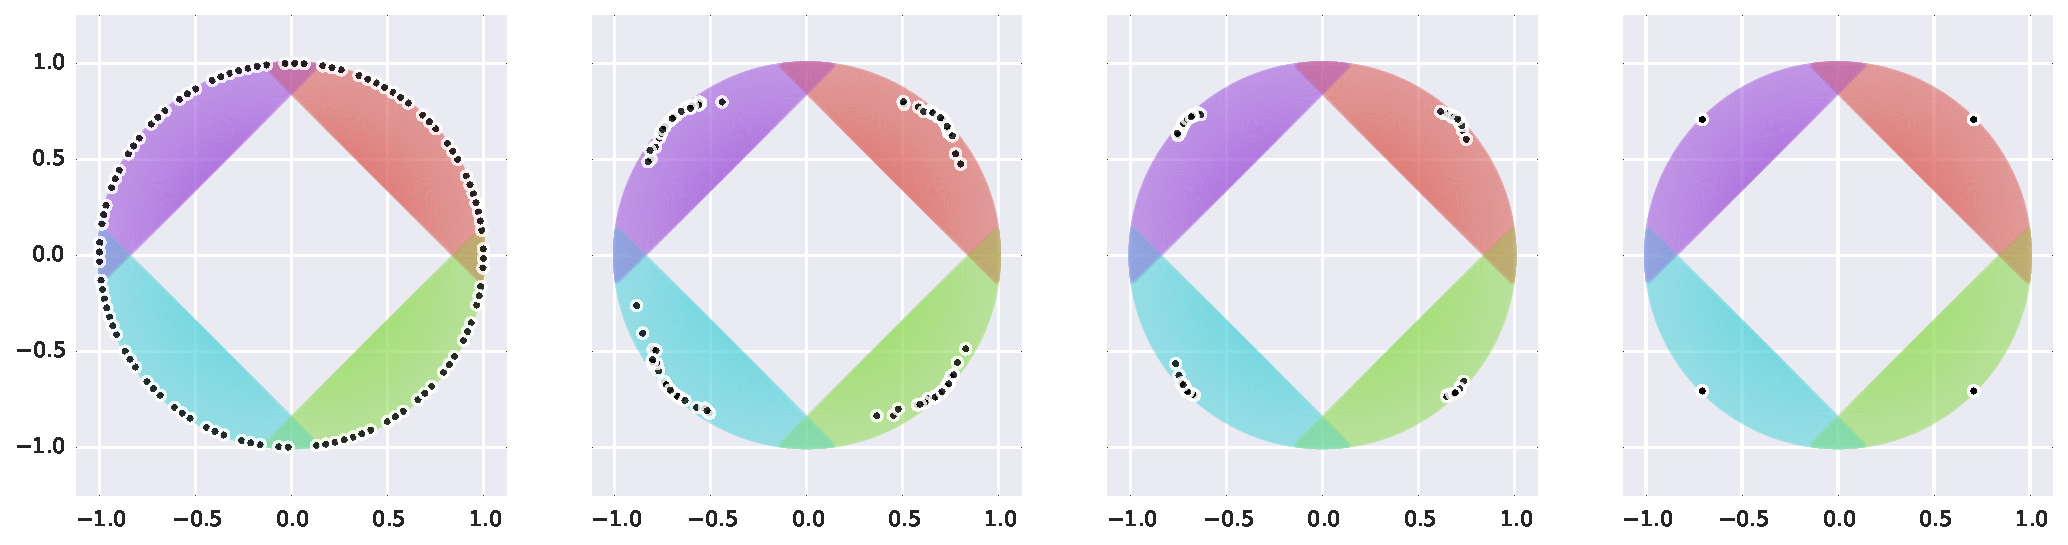
\includegraphics[width=\textwidth]{voja-spinnaker}
  \caption[Unsupervised learning of a two-dimensional representation.]{
The effect of Voja on the encoders of a 2-dimensional population, over time.
Each point corresponds to the encoder of one of \num{100} neurons.
Four input vectors are chosen of the form $(\pm 1 / \sqrt{2}, \, \pm 1 / \sqrt{2})$, and their areas of attraction within the unit circle are indicated by shaded regions ($c = 0.6$).
As the simulation progresses, from left to right, each encoder converges to one of the possible inputs.
Reproduced from \citet{knight2016}.
  \label{fig:voja-spinnaker}
    }

  \vspace{1em}

    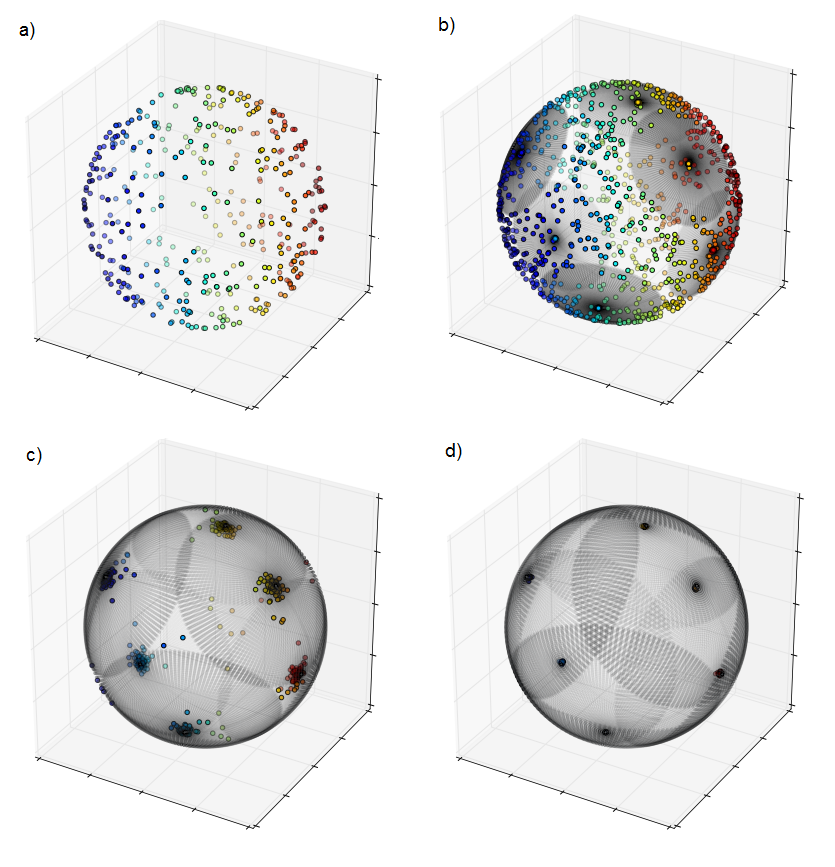
\includegraphics[width=0.5\textwidth]{voja-encoders}
    \caption[Unsupervised learning of a three-dimensional population.]{Input vector clustering of a 3-dimensional ensemble, presented with 6 evenly spaced $\V{x}$. (a)~The initial clustering, before any input has been given. (b)~Each input vector has been shown for two seconds of simulation time, with intercepts set to $\cos \left(\pi / 6 \right)$. Gray plates show the area of attraction for each input vector. (c)~Same as b, with intercepts chosen to give $p_i = 1/6$. (d)~Same as b, with intercepts set to $\cos \left( \pi / 3 \right)$. \label{e3d}
    Reproduced from \citet{voelker2014a}.
       \label{fig:voja-encoders}
    }
\end{figure}

\subsection{Supervised learning}
\label{sec:supervised}

This section has been adapted from preliminary work by \citet{voelker2015} and \citet{voelker2017c}.
This approach highlights the utility in shifting perspectives in learning to that of a dynamical system embedded within some larger function.
In particular, online learning is \emph{nothing more} than a dynamical system mapped onto localized computations manipulating state-variables within a network.
% State-variables are mapped onto weights, and their evolution is some function that depends on the weights.
We illustrate this by unifying Nengo's supervised learning and the NEF's dynamical systems framework at a theoretical level, and then leverage the resulting relationship in a practical spiking example with online learning.

The NEF typically learns its connection weights offline, but Nengo also supports a number of biologically-plausible supervised and unsupervised learning rules to learn these weights online~\citep{bekolay2011a}.
Prescribed Error Sensitivity~\citep[PES;][]{bekolay2013} is a biologically-plausible Hebbian supervised learning rule that is frequently used within Nengo models.
PES modifies the connection weights between populations of neurons to minimize an external (i.e.,~supervised) error signal.
It is equivalent in function to a single-layer application of gradient descent, applied online (i.e.,~stochastically) to its current input and supervised output.
This learning rule has been used to model episodic memory~\citep{trujillo2014}, hierarchical reinforcement learning~\citep{rasmussen2017}, adaptive motor control~\citep{komer2015, dewolf2016}, and many other tasks~\citep{aubin2018, choo2018}.
The PES learning rule is also partially supported by Loihi~[personal communication].

We solve the discrete dynamical system for the case of constant inputs and no noise, to show that the decoding vectors given by the NEF have a simple closed-form expression in terms of the number of simulation time-steps. Moreover, with $\gamma = (1 - \kappa \|\V{a}\|^2) < 1$, where $\kappa$ is the learning rate and $\V{a}$ is the vector of firing rates, the error at time-step $k$ is the initial error times $\gamma^k$. Thus, $\gamma > - 1$ implies exponential convergence to a unique stable solution, $\gamma < 0 $ results in oscillatory weight changes, and $\gamma \le -1$ implies instability.
\begin{lemma}[Dynamics of discrete unfiltered supervised learning]
\label{lemma:pes-dynamics}
{\normalfont \citep{voelker2015}}
Let $\gamma = (1 - \kappa \|\V{a}\|^2) < 1$, and $e_0 = y^* - \V{d}[0]^T \V{a}$, then:
\begin{align}
\label{eq:dk}
\V{d}[k] &= \V{d}[0] + e_0\frac{\V{a}}{\|\V{a}\|^2} (1 - \gamma^k)\text{, \quad $k \in \mathbb{N}$} \text{,}
\end{align}
and so the error at time-step $k$ is $y^* - \V{d}[k]^T \V{a} = e_0\gamma^k$. In particular, if $\gamma > - 1$, then $\V{d}[\infty]$ exists and is given by the unique solution,
\begin{align}
\label{eq:dinf}
\V{d}[\infty] &= \V{d}[0] + e_0\frac{\V{a}}{\|\V{a}\|^2} .
\end{align}
On the other hand, if $\gamma \le -1$ then the system is unstable.
The proof is given by \citet{voelker2015}.
\end{lemma}

Continuing this work, we solve for the dynamics of PES, while filtering the error with an arbitrary linear synapse model. 
For the most common case of a lowpass filter, the continuous-time weight changes happen to be characterized by a second-order bandpass filter with frequency $\omega = \sqrt{\tau^{-1} \kappa \|\V{a}\|^2 }$ and bandwidth $Q = \sqrt{\tau \kappa \|\V{a}\|^2 }$, where $\tau$ is the exponential time constant, $\kappa$ is the learning rate, and $\V{a}$ is the activity vector.
Therefore, the error converges to zero, yet oscillates if and only if $\tau \kappa \|\V{a}\|^2 > 1/4$.
This provides a heuristic for setting $\kappa$ based on the synaptic $\tau$, and a method for engineering remarkably accurate decaying oscillators using only a single spiking leaky integrate-and-fire neuron.

Lemma~\ref{lemma:pes-dynamics} fully characterized the discrete-time dynamics of PES under the restricted setting of a constant input signal, constant reference signal, and no noise.
Due to the absence of noise, no filter was required for the error signal.
However, for spiking networks considered in practice, a lowpass is applied to the error to filter out spike-noise~\citep[e.g.,][]{dewolf2016, rasmussen2017},  
We now relax the assumption of a constant reference signal, and apply an arbitrary linear filter to the error signal.
For simplicity, we do so for the case of a continuous-time simulation, but our analysis can also be applied to the discrete-time setting via the $\mathcal{Z}$-transform.
To keep our analysis tractable, we still assume a constant input signal, and briefly discuss implications for the general dynamic setting.

We begin by formulating a mathematical description of the network, present our theoretical results, prove them mathematically, validate them with numerical simulations, and demonstrate the utility of this analysis by engineering oscillators with predetermined frequencies and decay rates.
Finally, we conclude by discussing some implications for learning spiking dynamical networks online.

\subsubsection{Prescribed Error Sensitivity}

\fig{pes-filtered-network}{0.5}{Supervised learning rule analyzed as a dynamical system.}{
  Network diagram used to analyze the PES rule.
  A constant input $x$ is represented by a population of $n$ spiking neurons with the activity vector $\V{a} \in \mathbb{R}^n$.
  A dynamic reference signal $r(t)$ determines the error $e(t) = \left((y - r) \ast h\right)(t)$~(equation~\ref{eq:error}), which in turn drives $y(t)$ towards $r(t)$ by modulating the connection weights via PES~(equation~\ref{eq:pes}).
  These learned connection weights decode $y(t)$ via the decoders $\V{d}(t) \in \mathbb{R}^n$~(equation~\ref{eq:decoding}).
  A linear filter $h(t)$ models the post-synaptic current induced by each spike.
  Reproduced from \citet[][Figure~1]{voelker2017c}.
}

Consider a network containing a population of $n$ spiking neurons, encoding the constant scalar input $x$.
Let $\V{a} \in \mathbb{R}^n$ be the average (i.e.,~rate) activity of each neuron in response to this encoding.\footnote{Here on, we assume that $\V{a} \ne \V{0}$, otherwise PES will have no effect.}
This vector is determined by the first principle of the NEF, and remains fixed for constant $x$.
The \emph{decoders} $\V{d}(t) \in \mathbb{R}^n$ determine the scalar output $y(t)$ via the dot-product:
\begin{equation}
\label{eq:decoding}
y(t) = \transpose{\V{a}} \V{d}(t)  \text{.}
\end{equation}
The PES rule learns these decoders, online, according to the following dynamics:
\begin{equation}
\label{eq:pes}
\dot{\V{d}}(t) = -\kappa e(t) \V{a} \text{,}
\end{equation}
where $\kappa > 0$ is the learning rate,\footnote{$\kappa$ is automatically scaled by $n^{-1}$ in Nengo, to balance the linear scaling of $\|\V{a}\|^2$.} and $e(t)$ is the chosen error signal:\footnote{Signs are flipped in \citet{voelker2015}; equations~\ref{eq:pes} and~\ref{eq:error} are consistent with Nengo.}
\begin{equation}
\label{eq:error}
e(t) = \left((y - r) \ast h \right)(t) \text{,}
\end{equation}
where $r(t)$ is the reference (i.e.,~ideal) output, and $h(t)$ is some arbitrary linear filter modeling the post-synaptic current (PSC) induced by a spike arriving at the synaptic cleft.
Typically, $h(t)$ is a first-order lowpass filter with time constant~$\tau > 0$ (i.e.,~equation~\ref{eq:lowpass-laplace}):
\begin{equation}
\label{eq:lowpass}
h(t) = \frac{1}{\tau} e^{-\frac{t}{\tau}} \iff H(s) = \frac{1}{\tau s + 1} \text{.}
\end{equation}
%Thus, the connection weights learn to represent $r$ when presented with $x$.
The final network is summarized in Figure~\ref{fig:pes-filtered-network}.
This also naturally extends to the case where $x$ and $y$ are vectors (using a population code), but we consider the scalar case for simplicity. 

Now, we aim to characterize the dynamics of $e(t)$ in response to the control signal $r(t)$.
Alternatively, we could characterize the dynamics of $y(t)$ or $\V{d}(t)$, but the former is easier to work with, while describing the latter via equations~\ref{eq:decoding} and~\ref{eq:pes} (i.e.,~by integrating $e(t)$).

\begin{theorem}[Dynamics of supervised learning with continuous filtered feedback]
\label{thm:pes-filtered}
{\normalfont \citep{voelker2017c}}
Let $\phi = \tau \kappa \|\V{a}\|^2$.
For the network described in Figure~\ref{fig:pes-filtered-network}, we have:
\begin{equation}
\label{eq:time-domain}
e(t) = (r \ast f)(t) \text{,}
\end{equation}
where: %\footnote{$\mathcal{L}^{-1} \left\{ \cdot \right\}$ denotes the inverse Laplace transform.}
\begin{equation}
\label{eq:s-domain}
F(s) = \frac{-s}{s H(s)^{-1} + \kappa \|\V{a}\|^2} \text{,} 
%f(t) &= \mathcal{L}^{-1} \left\{ F(s) \right\} \\
%H(s) &= \mathcal{L} \left\{ H(t) \right\} \text{.}
\end{equation}
hence $F(s)$ is the transfer function from $R(s)$ to $E(s)$.
For the case of a first-order lowpass filter (equation~\ref{eq:lowpass}),
\begin{align}
\label{eq:lowpass-solution}
\implies \quad F(s) = \frac{-s}{\tau s^2 + s + \kappa \|\V{a}\|^2} &= \frac{-\left( \kappa \|\V{a}\|^2 \right)^{-1} s}{\left(\frac{1}{\omega^2}\right)s^2 + \left(\frac{1}{\omega Q}\right) s + 1} \quad\quad \\
\omega &= \sqrt{\tau^{-1} \kappa \|\V{a}\|^2 } \label{eq:bandpass-w} = \tau^{-1} \sqrt{\phi} \\
Q &= \sqrt{\tau \kappa \|\V{a}\|^2 } = \sqrt{\phi} \label{eq:bandpass-Q} \text{.}
\end{align}
Thus, $F(s)$ is a second-order $Q$-bandpass filter with frequency $\omega$ in radians per second ($\frac{\omega}{2 \pi}$ is the frequency in hertz)~\citep[][pp.~8.9--8.10]{zumbahlen2011linear}.
The poles of $F(s)$ are:
\begin{equation}
\label{eq:poles}
s = \frac{-1 \pm \sqrt{1 - 4 \phi}}{2\tau} \text{.}
\end{equation}
%with complex magnitude $|s| = \omega$.
Since $\phi > 0$, this system is exponentially stable, and, moreover, the impulse response, $f(t)$, is a decaying oscillator if and only if $\phi > 1/4$.
\end{theorem}

\begin{proof}
We begin by transforming equations~\ref{eq:decoding}--\ref{eq:error} into the Laplace domain:
\begin{align*}
Y(s) &= \transpose{\V{a}} \V{D}(s) \\
s\V{D}(s) &= - \kappa E(s) \V{a} \\
E(s) &= \left(Y(s) - R(s) \right) H(s) \text{.\footnotemark}
\end{align*}
\footnotetext{This has nice form since $\V{a}$ is a constant -- otherwise multiplication of two time-varying signals becomes a complex integral in the Laplace domain.}%
Substituting the first two equations into the last, yields:
\begin{align*}
&& E(s) &= \left( \transpose{\V{a}} \V{D}(s) - R(s) \right) H(s) \\
&& &= \left( - \transpose{\V{a}} s^{-1} \kappa E(s) \V{a} - R(s) \right) H(s) \\
&& &= - \kappa \|\V{a}\|^2 s^{-1} H(s) E(s) - R(s) H(s) \\
\iff && \left(1 + \kappa \|\V{a}\|^2 s^{-1} H(s) \right) E(s) &= - R(s) H(s) \\
\iff && E(s) &= R(s) \left( \frac{-H(s)}{1 + \kappa \|\V{a}\|^2 s^{-1} H(s)} \right) \\
&& &= R(s) \left( \frac{- s}{s H(s)^{-1} + \kappa \|\V{a}\|^2} \right) \\
&& &= R(s) F(s) \text{.} % \tag*{\qed}
\end{align*}

Equations~\ref{eq:time-domain} and~\ref{eq:s-domain} follow from the convolution theorem.
Equations~\ref{eq:lowpass-solution}--\ref{eq:bandpass-Q} are verified by substituting $H(s)^{-1} = \tau s + 1$ into equation~\ref{eq:s-domain}.

The poles of the system (equation~\ref{eq:poles}) are obtained by applying the quadratic formula to the denominator polynomial from equation~\ref{eq:lowpass-solution} ($\tau s^2 + s + \kappa \|\V{a}\|^2$).
%The magnitude of the poles ($\omega$) come from the polar coordinate solution to this quadratic.
Exponential stability is implied by both poles being strictly in the left half-plane.
Lastly, $f(t)$ oscillates if and only if the poles are complex, if and only if the discriminant ($1 - 4 \phi$) is negative, if and only if $\phi > 1 / 4$.
\end{proof}

%As a corollary to equation~\ref{eq:lowpass-solution} and the Laplace transform of equations~\ref{eq:decoding} and~\ref{eq:pes},
%\begin{equation}
%y(t) = (r \ast g)(t) \text{,}
%\end{equation}
%where:
%\begin{equation}
%G(s) = \frac{\kappa \|a\|^2}{\tau s^2 + s + %\kappa \|\V{a}\|^2} \text{,}
%\end{equation}
%which has the same dynamics as equation~\ref{eq:lowpass-solution} with a phase shift.
%But these are (unfiltered) spikes...

\subsubsection{Validation}

We construct the network from Figure~\ref{fig:pes-filtered-network} using Nengo, with only $n = 1$ spiking leaky integrate-and-fire neuron (mean firing rate of $262\,$Hz),\footnote{%
Spikes are used in place of $\V{a}$ in equations~\ref{eq:decoding} and~\ref{eq:pes}.} $\tau = 0.1\,$s (equation~\ref{eq:lowpass}), $x = 0$, and $\kappa$ such that $\phi > 1/4$.
We construct the transfer function from equation~\ref{eq:lowpass-solution} using NengoLib:
\begin{python}
import nengolib
from nengolib.signal import s
H = nengolib.Lowpass(tau)
F = -s / (s/H + kappa*a.dot(a))
\end{python}
where \texttt{tau}~$\leftarrow \tau$ is the time constant of the synapse, \texttt{kappa}~$\leftarrow \kappa$ is the learning-rate supplied to Nengo (divided by $n$), and \texttt{a}~$\leftarrow \V{a}$ is the NumPy array for the population's activity.
We evaluate $(r \ast f)(t)$ using \texttt{F.filt(r, dt=dt)}, and compare this to the $e(t)$ obtained numerically in simulation.
The \texttt{filt} method automatically discretizes $F(s)$ according to the simulation time-step (\texttt{dt}~$= 1\,$ms) using zero-order hold (ZOH).\footnote{Technically, for a discrete-time simulation, the problem and results should have been formulated in the discrete-time domain using the $Z$-transform to begin with, as opposed to discretizing at the end, but the difference is quite subtle.}

In Figure~\ref{fig:pes-error}, we confirm that $(r \ast f)(t)$ approximates the numerical $e(t)$ given white noise $r(t)$.
In Figure~\ref{fig:pes-oscillator}(Top), we exploit our knowledge of the impulse response, $f(t)$, to engineer a number of decaying oscillators by controlling $r(t)$.
In Figure~\ref{fig:pes-oscillator}(Bottom), we evaluate \texttt{np.abs(F.evaluate(freqs))} at a variety of frequencies (\texttt{freqs}) to visualize the bandpass behaviour of each filter.

\fig{pes-error}{1.0}{Validating the dynamical system describing supervised learning.}{
  Comparison of the analytical error (equation~\ref{eq:lowpass-solution}) to the numerical $e(t)$ obtained by simulating the network from Figure~\ref{fig:pes-filtered-network} ($\kappa = \numprint{e-3}$).
  The control signal $r(t)$ is randomly sampled white noise with a cutoff frequency of $10\,$Hz.
  The normalized root-mean-square error is approximately $3.7\%$.
  Reproduced from \citet[][Figure~2]{voelker2017c}.
}

\fig{pes-oscillator}{1.0}{Leveraging the dynamics of learning to produce oscillations.}{
  Harnessing the dynamics of PES with various $\kappa$ to engineer decaying oscillators with predetermined frequencies ($\omega$) and bandwidths ($Q$), using only a single leaky integrate-and-fire neuron.
  The time constant of the first-order lowpass filter is fixed at $\tau = 0.1\,$s, while $\kappa$ is set to achieve the desired $\omega$ via equation~\ref{eq:bandpass-w}.
  (Top)~Once every second, $r(t)$ is set to a unit-area impulse.
  Consequently, $e(t)$ oscillates according to the impulse response, $f(t)$.
  (Bottom)~Visualizing the ideal frequency response of $F(s)$ (equation~\ref{eq:lowpass-solution}).
  Dashed lines at $\omega$ (equation~\ref{eq:bandpass-w}) align with the peak of each bandpass filter, or equivalently the frequency of each oscillation.
  The width of each filter is proportional to the decay rate $Q^{-1}$ (equation~\ref{eq:bandpass-Q}).
  Reproduced from \citet[][Figure~3]{voelker2017c}.
}

\subsubsection{Discussion}

Since $\phi = \tau \kappa \|\V{a}\|^2 > 1/4$ if and only if the weights oscillate, this motivates a simple heuristic for setting the learning rate to prevent oscillatory weight changes: set $\kappa \le \frac{1}{4 \tau \|\V{a}\|^2}$, where $\|\V{a}\|^2$ is maximal over all possible activity vectors.
In this case, equation~\ref{eq:lowpass-solution} factors into a (differentiated) double-exponential:
\begin{equation*}
F(s) = \frac{-\tau_1 \tau_2 s}{\tau (\tau_1 s + 1)(\tau_2 s + 1)} = \left( - \tau_1 \tau_2 \tau^{-1} s \right) \left( \frac{1}{\tau_1 s + 1}\right) \left(\frac{1}{\tau_2 s + 1}\right) \text{,}
\end{equation*}
that is, two first-order lowpass filters chained together, where:
\begin{equation*}
\left( \tau_1, \tau_2 \right) = \frac{2 \tau}{1 \mp \sqrt{1 - 4 \phi}} \text{,}
\end{equation*}
by equation~\ref{eq:poles}.
In other words, the non-oscillatory regime ($0 < \phi \le 1/4$) of PES is characterized by the dynamics of a double-exponential.
We remark that $\tau_1 = \tau_2 = 2 \tau$ (i.e.,~an alpha filter) directly on the point of bifurcation from double-exponential to oscillatory behaviour ($\phi = 1/4$; see Figure~\ref{fig:pes-poles}).

In all applications involving online learning (that we are aware of) oscillatory weight changes are viewed as problematic, and so the relevant constants ($\tau$, $\kappa$, and $\| \V{a} \|^2$) are tweaked until the issue disappears.
In contrast, we have shown that not only can the relationship between these constants and the oscillations be fully understood, but they can be harnessed to engineer bandpass filters (with respect to the transformation $r(t) \mapsto e(t)$) with specific frequencies ($\omega$) and bandwidths ($Q$).
More generally, the PES learning rule can be used to construct dynamical systems whose transfer function (equation~\ref{eq:s-domain}) depends on $H(s)$, $\kappa$, and $\| \V{a} \|^2$.
As we used only a single spiking neuron, the accuracy of these systems rely solely on the accuracy of the PES implementation, the model of $H(s)$, and the constancy of $(\V{a} \ast h)(t)$ in practice (i.e.,~given spiking activity).

Although we have analyzed the continuous-time setting, the same proof technique can be applied to the discrete-time domain by use of the $Z$-transform.
Likewise, although we have assumed $x$ is a constant, we can apply a ``separation of time-scales'' argument (i.e.,~assuming $x(t)$ changes on a slower time-scale than $f(t)$) to carry this same analysis over to dynamic $x(t)$.
%More precisely, bounding the real components of equation~\ref{eq:poles} above by $c$,
%\footnote{Strictly, $c = -\frac{1}{2\tau}$ for the oscillatory case, and $c = \frac{-1 + \sqrt{1 - 4 \tau \kappa \|\V{a}\|^2}}{2 \tau}$ otherwise.}
By equation~\ref{eq:poles}, this analysis holds approximately for $x(t)$ with frequencies $\ll \left(4 \pi \tau \right)^{-1}$\,Hz, by applying a time-varying filter to $\V{d}(t)$ that depends on the current activity vector.
Incidentally, this bound is only half that of our definition of low-frequency representation from section~\ref{sec:energy-minimization}.

In conclusion, we have extended our previous analysis of PES to include linearly filtered feedback and a dynamic reference signal.
This fully characterizes the rule in the context of NEF networks representing a constant value, as a transfer function from the reference signal to the error signal.
This transfer function may then be readily analyzed and exploited using linear systems theory, to instantiate oscillators using far fewer resources (i.e.,~a single neuron coupled with a local learning rule) than what would be needed to achieve the same level of precision with a recurrent SNN implementing the same dynamical system.
This demonstrates a more general principle of recurrently coupling available dynamical primitives in biological models (here, a PSC that is integrated by an online learning rule) to improve network-level computations.
% If we can find ways to exploit these things, then nature almost certainly can...

Many other aspects of NEF networks may also be analyzed from a dynamical systems perspective.
For instance, the dynamics of the representational error, the chaotic dynamics of voltage traces, or the undecidable attractor dynamics induced by neural saturation~(see section~\ref{sec:chaos}).
We do not go into detail here.
We mention this because, similar to our lessons learned in the above discussion, it may become important to have the ability to systematically characterize and subsequently leverage the dynamics that are already naturally present in the network's function.

\fig{pes-poles}{0.4}{Bifurcation analysis of oscillations from learning.}{
  Visualizing the poles of $F(s)$ (equation~\ref{eq:poles}) by sweeping $\kappa > 0$ (while $\| \V{a} \|^2$  and $\tau = 0.1\,$s remain fixed).
  Arrows follow the direction of \emph{increasing} $\kappa$.
  When $\phi \le \frac{1}{4}$, the dynamics of PES are a double-exponential.
  The learning rule becomes an alpha filter when the two poles collide: $\phi = \frac{1}{4} \iff s = -\frac{1}{2\tau}$ (marked by a solid circle).
  When $\phi > \frac{1}{4}$, the weight changes become oscillatory (due to complex poles).
  As $\kappa$ increases, the oscillatory frequency, $\omega$, scales as $\mathcal{O}\left(\sqrt{\kappa}\right)$.
  As $\kappa$ decreases, the first pole converges to $s = -\frac{1}{\tau}$ (marked by a solid \texttt{x}) while the second pole cancels the zero at $s = 0$. %(i.e.,~$F(s) = -H(s)$, $s \ne 0$).
  Reproduced from \citet[][Figure~4]{voelker2017c}.
}

\subsection{Optimization}

There is extensive literature on the general topic of implementing optimization algorithms in the form of dynamical systems, dating back at least to the work of \citet{brockett1991dynamical}.
% But we are not aware of any reviews at this level where we are concerned with implementation details into consideration.
\citet{voelkerimplementing} noticed that the ``hill climbing'' algorithm may be cast as a dynamical system, and leveraged this to construct an SNN that locally searches across an error landscape.
This observation naturally extends to any gradient-based algorithm, since these algorithms are expressed as state-vectors that update continuously according to some (possibly nonlinear) function of the state of the system. 
Instances of this include gradient descent, feedback alignment~\citep{stockel2019align}, Bayesian inference, and expectation-maximization~\citep{sharma2017}.

Apart from what has been done in the NEF, there exist many other dynamical systems that solve optimization problems, that could just as easily be realized using Principle 3, including:
compressed sensing~\citep{kim2007interior},
sparse coding~\citep[LASSO;][]{shapero2014optimal, tang2017sparse},
dictionary learning~\citep{lin2018dictionary},
Hopfield networks~\citep{hopfield1982, frady2019robust},
non-negative similarity matching~\citep{pehlevan2019spiking},
and various other algorithms related to eigenvalues,
% principle component analysis,
independent component analysis,
and non-negative matrix factorization.
But rather than focusing on any one of these algorithms in particular, we turn our efforts to developing a comprehensive understanding of how the NEF may be extended to implement all of them.

\chapter{Extensions to the Neural Engineering Framework}
\label{chapt:nef-extensions}

Rapid growth in the field of neuromorphic engineering---over the past 30 years~\citep{mead1988silicon}---has accelerated the production of a large variety of neuromorphic architectures, each with distinct constraints and trade-offs that impact the degree of programmability and performance as a function of energy-consumption (section~\ref{sec:neuromorphic}).
Among these considerations, are issues involving:
discretization (in time), quantization (truncation of both neural states and weight matrices), connectivity constraints, memory constraints, volume of spike traffic, external input-output bandwidth and delays, thermal variability, transistor mismatch, conversion of analog signals to digital pulses, and the introduction of higher-order dynamics throughout.
The NEF already solves many of these problems in theory with varying degrees of success in practice.
The focus of this chapter is to expose our novel contributions to solving these problems in the context of extending the scope of Principle~3.
The intent is to bolster up the NEF with a variety of additional methods and techniques for analyzing and leveraging spiking dynamical computations.

\section{Synapses}
\label{sec:synaptic-extensions}

This section has been adapted from the works of \citet[][patent pending]{dynamicspatent}, \citet{voelker2017iscas}, \citet{voelker2017neuromorphic}, and \citet{voelker2018}.
Here, we focus on a dynamical primitive of SNNs known as the synapse model, $h(t)$, and address many of the differences that emerge between the idealization made by the NEF and the realities imposed by neuromorphic hardware (and often too, the brain).
This leads to several high-level results that exploit their higher-order dynamics, account for time-constant mismatch, leverage their heterogeneity, and solve for optimal filters.

\subsection{Linear transfer functions}
\label{sec:linear-extensions}

We build a comprehensive theory, adapted from \citet{voelker2018}, for including arbitrary linear synapse models in the neural architecture.
This is applied to the case of implementing linear systems, but many of these same techniques also carry over to later sections in the case of nonlinear systems. % the case of nonlinear dynamical systems with heterogeneous synapses~\citep{voelker2017iscas, voelker2017neuromorphic}.

Consider the linear time-inviant~(LTI) system (repeating equation~\ref{eq:lti}, for clarity):
\begin{equation} \label{eq:lti-repeated}
\begin{split}
\dot{\V{x}}(t) &= A\V{x}(t) + B\V{u}(t) \\
\V{y}(t) &= C\V{x}(t) + D\V{u}(t) \text{.}
\end{split}
\end{equation}
This state-space model is related to its \emph{transfer function}, $F(s)$, which uniquely characterizes its input-output response in the Laplace domain according to
$$
F(s) = \laplace{f(t)}(s) = \frac{\laplace{\V{y}(t)}(s)}{\laplace{\V{u}(t)}(s)} = \frac{\V{Y}(s)}{\V{U}(s)} \text{,}
$$
by the following equation~\citep{brogan1982modern}:
\begin{align} \label{eq:ss2tf}
F(s) = C(sI - A)^{-1}B + D \text{.}
\end{align}
Now let $F(s)$ be the transfer function for the linear dynamics that we wish to implement (derived by equations~\ref{eq:lti-repeated} and~\ref{eq:ss2tf}), and let $H(s)$ be the transfer function for an arbitrary linear synapse model ($H(s) = \mathcal{L} \left\{ h(t) \right\}$).
As stated in section~\ref{sec:principle3}, introducing the synapse model means replacing the integrator ($s^{-1}$) with $H(s)$.
This is equivalent to replacing $s$ with $H(s)^{-1}$.
Notably, substituting $H(s)$ for the integrator results in the transfer function $F \left( H(s)^{-1} \right)$, which no longer implements the original, desired dynamics $F(s)$. %, via the change-of-variables $s \longleftrightarrow H(s)^{-1}$.
However, we would like to ensure that the new dynamics match the originally specified $F(s)$.
The key insight is that we can determine a new function, $F^H(s)$, such that $F^{H}\left( H(s)^{-1} \right) = F(s)$.
That is, we can solve for a function that provides the original dynamics when implemented using the transfer function $H(s)$ as the dynamical primitive.
This is formalized by the following definition:
\begin{definition} \label{def:maps-onto}
A function $F^{H}(s)$ \emph{maps $F$ onto $H$} if and only if it satisfies:
\begin{align} \label{eq:maps-onto}
F^{H}\left( \frac{1}{H(s)} \right) = F(s) \text{.}
\end{align}
\end{definition}

This definition compactly expresses the notion of a ``change of dynamical primitive'', in that $F(s)$ is mapped from the canonical primitive, $s^{-1}$, onto some new primitive, $H(s)$.
Trivially, $F(s)$ maps itself onto $s^{-1}$.
Non-trivial examples are given below.
%To see this, we apply the key insight to some $F^{H}(s)$ to reveal that substituting the integrator for the synapse results in the dynamics $F^{H}(H(s)^{-1})$, which is equal to $F(s)$ if and only if it maps $F$ onto $H$, by definition~\ref{def:maps-onto}.
%Then, to compensate for this change in dynamics, we must solve for some transfer function $F^{H}(s)$ that satisfies definition~\ref{def:maps-onto}.
%This effectively means inverting the change-of-variables $s \longleftrightarrow H(s)^{-1}$.

Once we identify a $F^{H}(s)$ that maps $F$ onto $H$, any state-space model $\left( A^H\text{,}\, B^H\text{,}\, C^H\text{,}\, D^H \right)$ that satisfies
\begin{equation} \label{eq:ss-mapped}
F^{H} \left( s \right) = C^H \left( sI - A^H \right)^{-1}B^H + D^H
\end{equation}
will implement the desired dynamics when using $H(s)$ as the dynamical primitive, by equations~\ref{eq:ss2tf} and~\ref{eq:maps-onto} (see Figure~\ref{fig:lti-system-mapped-general}).

\begin{figure}
  \centering
  \resizebox{\columnwidth}{!} {
	\begin{tikzpicture}[auto, node distance=2cm,>=latex']
	  \node [input, name=input] {};
	  \node [coordinate, name=fanin, right of=input] {};
	  \node [block, right of=fanin, node distance=1.5cm] (B) {$B^H$};
	  \node [sum, right of=B, node distance=2cm] (sum) {$+$};
	  \node [block, right of=sum, node distance=2cm] (integ) {$H(s)$};
	  \node [block, right of=integ, node distance=3.5cm] (C) {$C^H$};
	  \node [sum, right of=C, node distance=2cm] (sumout) {$+$};
	  \node [output, right of=sumout] (output) {};
	
	  \node [block, below of=integ] (A) {$A^H$};
	  \node [block, above of=integ] (D) {$D^H$};
	
	  \draw [-] (input) -- node {$\V{u}$} (fanin);
	  \draw [->] (fanin) -- node {} (B);
	  \draw [->] (fanin) |- (D);
	  \draw [->] (D) -| node {} (sumout);
	  \draw [->] (B) -- node {} (sum);
	  \draw [->] (sum) -- node {} (integ);
	  \draw [->] (integ) -- node [name=fanout] {$\V{x}$} (C);
	  \draw [->] (fanout) |- (A);
	  \draw [->] (A) -| node {} (sum);
	  \draw [->] (C) -- node {} (sumout);
	  \draw [->] (sumout) -- node {$\V{y}$} (output);
	\end{tikzpicture}  
  }
  \caption[Extending Principle~3 to arbitrary linear synapses.]{ \label{fig:lti-system-mapped-general}
    Block diagram for an LTI system, equivalent to Figure~\ref{fig:lti-system}, with the integrator replaced by a more general linear filter $H(s)$.
    The state-space model $\left( A^H\text{,}\, B^H\text{,}\, C^H\text{,}\, D^H \right)$ is obtained from some transfer function $F^{H}(s)$ that maps $F$ onto $H$, as defined in the text.
    This generalizes Figure~\ref{fig:lti-system-mapped} to arbitrary linear synapse models.
    Reproduced from \citet[][Figure~7]{voelker2018}.
  }
\end{figure}

Therefore, supposing $F^{H}(s)$ satisfies definition~\ref{def:maps-onto}, and that it is convertible to a state-space model (equation~\ref{eq:lti}), then Figure~\ref{fig:lti-system-mapped-general} is just another form of Figure~\ref{fig:lti-system}, but with the integrator replaced by the synapse.
Note that this construction, on its own, does not specify how to find a satisfying $F^{H}(s)$, nor whether such a function exists, nor whether it can be converted to a state-space model.
We provide several examples leading to such a specification at the end of this section.
%This will be made clear through a number of examples, culminating with an approach that recovers an important result from linear systems theory (see appendix~\ref{app:discrete-connection}).
%In appendix~\ref{app:state-space} we discuss our freedom to choose state-space models, and the connection to choice of encoders in the NEF.

Before proceeding, we remark that the above theory directly carries over from the continuous-time domain to the discrete-time domain.
The discrete-time formulation of an LTI system is similar to equation~\ref{eq:lti}, but increments time in steps of length $\dt{}$:
\begin{equation} \label{eq:dlti}
\begin{split}
\V{x}[t+\dt{}] &= \bar{A}\V{x}[t] + \bar{B}\V{u}[t] \\
\V{y}[t] &= \bar{C}\V{x}[t] + \bar{D}\V{u}[t] \text{,}
\end{split}
\end{equation}
where the discrete state-space model $\left( \bar{A}\text{,}\, \bar{B}\text{,}\, \bar{C}\text{,}\, \bar{D} \right)$ fully defines the system.
The discrete-time equivalent to the Laplace transform is the $\mathcal{Z}$\emph{-transform}, named for its use of the variable $z$ to denote the complex frequency domain.
In this domain, $z^{-1}$ plays the role of $s^{-1}$, by performing a discrete shift forwards, one step in time (i.e.,~a delay of one time-step), instead of integration.
A well-known result is that the transfer function of this discrete LTI system---defined as the ratio of the $\mathcal{Z}$-transform of the output to the $\mathcal{Z}$-transform of the input---is equal to $F(z) = \bar{C} (zI - \bar{A})^{-1} \bar{B} + \bar{D}$, analogously to equation~\ref{eq:ss2tf}.
Consequently, all of the previous discussion carries over to discrete LTI systems.
In particular, for a discrete synapse expressed using the $\mathcal{Z}$-transform, $H(z)$, we have the analogous definition:
\begin{definition} \label{def:discrete-maps-onto}
A function $F^{H}(z)$ \emph{maps $F$ onto $H$} if and only if it satisfies:
\begin{align} \label{eq:discrete-maps-onto}
F^{H}\left( \frac{1}{H(z)} \right) = F(z) \text{.}
\end{align}
\end{definition}
Given some $F^{H}(z)$ that maps $F$ onto $H$, any state-space model $\left( \bar{A}^H\text{,}\, \bar{B}^H\text{,}\, \bar{C}^H\text{,}\, \bar{D}^H \right)$ that satisfies
\begin{equation} \label{eq:dss-mapped}
F^{H} \left( z \right) = \bar{C}^H \left( zI - \bar{A}^H \right)^{-1}\bar{B}^H + \bar{D}^H
\end{equation}
will implement the desired dynamics $F(z)$ when using $H(z)$ as the dynamical primitive.
Hence, the task of determining $F^{H}(\cdot)$ is identical for both continuous- and discrete-time domains---it is only $F(\cdot)$ and $H(\cdot)$ that differ.

\subsubsection{Continuous lowpass synapse}

The first example we consider demonstrates that our new theory recovers the standard form of Principle~3 from the NEF (see section~\ref{sec:principle3}).
For the case of a continuous-time first-order lowpass filter (equation~\ref{eq:lowpass}), $H(s) = \left(\tau s + 1 \right)^{-1}$, let:
\begin{align*}
F^H(s) &:= C \left( sI - (\tau A + I) \right)^{-1} \left( \tau B \right) + D \\
&= C \left( \left(\frac{s-1}{\tau}\right)I - A \right)^{-1}B + D \text{.}
\end{align*}
Then, 
\begin{align*}
F^H \left( \tau s + 1 \right) &= C \left( \left(\frac{(\tau s + 1) - 1}{\tau}\right) I - A \right)^{-1}B + D \\
&= F(s)\text{,} 
\end{align*}
which satisfies definition~\ref{def:maps-onto}.
Therefore, by equation~\ref{eq:ss-mapped},
\begin{equation} \label{eq:p3-novel}
\begin{aligned}
A^H &= \tau A + I \text{,} & \quad C^H &= C \text{,} \\
B^H &= \tau B \text{,} & \quad D^H &= D \text{.}
\end{aligned}
\end{equation}
%$A^H = \tau A + I$, $B^H = \tau B$, $C^H = C$, and $D^H = D$.
This completes our novel proof of Principle~3 from section~\ref{sec:principle3}.

\subsubsection{Discrete lowpass synapse}

When simulating any NEF network on a digital computer, we necessarily use time-steps of finite length $\dt{} > 0$ to advance the state of the network, updating at discrete moments in time~\citep{bekolay2014}.
For instance, Nengo currently uses a default of $\dt{} = 1$\,ms, and implements a zero-order hold~(ZOH) discretization of the synaptic filter.
Implementing ZOH means that all continuous-time signals are held constant within each time-step.
This discretization of equation~\ref{eq:lowpass} gives:
\begin{equation}
H(z) = \frac{1 - a}{z - a} \text{,} \quad a := e^{-\frac{\dt{}}{\tau}} \text{.} \nonumber
\end{equation}
If our desired transfer function is expressed in continuous-time, $F(s)$, then we should also discretize it to $F(z) = \bar{C} (zI - \bar{A})^{-1} \bar{B} + \bar{D}$, with the same time-step, and again using ZOH discretization for consistency.
Let,
\begin{align*}
F^H(z) &:= \bar{C} \left(zI - \frac{1}{1 - a} \left(\bar{A} - aI \right) \right)^{-1} \left( \frac{1}{1-a}\bar{B} \right) + \bar{D} \\
&= \bar{C} \left( \left(z(1 - a) + a \right)I - \bar{A} \right)^{-1}\bar{B} + \bar{D} \text{.}
\end{align*}
Then, 
\begin{align*}
F^H \left( \frac{z-a}{1-a} \right) &= \bar{C}\left( \left( \frac{z-a}{1-a}(1 - a) + a \right)I - \bar{A} \right)^{-1}\bar{B} + \bar{D} \\
&= F(z) \text{,}
\end{align*}
which satisfies definition~\ref{def:discrete-maps-onto}.
Therefore, by equation~\ref{eq:dss-mapped},\begin{equation} \label{eq:discrete-p3}
\begin{aligned}
\bar{A}^H &= \frac{1}{1 - a} \left(\bar{A} - aI\right) \text{,} & \quad \bar{C}^H &= \bar{C} \text{,} \\
\bar{B}^H &= \frac{1}{1-a}\bar{B} \text{,} & \quad \bar{D}^H &= \bar{D} \text{,}
\end{aligned}
\end{equation}
provides an exact implementation of the desired system for digital architectures, regardless of the simulation time-step (assuming ZOH).
% Consequently, we use this method in the simulations reported in this paper unless otherwise noted.

\subsubsection{Delayed continuous lowpass synapse}

Next, we consider a continuous-time first-order lowpass filter with a time-delay of $\lambda$:
\begin{equation} \label{eq:delayed-lowpass}
H(s) = \frac{e^{-\lambda s}}{\tau s + 1} \text{.}
\end{equation}
This same model has been proposed by \citet[][equation~6.2]{roth2009modeling} as a more realistic alternative to equation~\ref{eq:lowpass}, that includes an axonal transmission delay of length $\lambda$ (on the order of $\tau$) to account for the finite-velocity propagation of action potentials.
By commutativity of convolution, modeling the delay in the synapse (as in equation \ref{eq:delayed-lowpass}) is equivalent to modeling the delay in spike propagation.
Equation~\ref{eq:delayed-lowpass} may also be used to account for feedback delays within some broader setting (e.g.,~when the feedback term is computed via some delayed system).

In the mammallian cortex, $\lambda$ is known to range between $0.1$--$44$\,ms while being precise and reproducible~\citep{lagorce2015stick}.
In analog circuitry, $\lambda$ grows in proportion to the square of the wire length, and is necessarily introduced by the pulse-extension of digital-to-analog circuits~\citep{voelker2017iscas}.
This delay term may also be configured on digital architectures such as Loihi~\citep{davies2018loihi}.

Letting $d := \frac{\lambda}{\tau}e^{\frac{\lambda}{\tau}}$, and $W_0(\cdot)$ denote the principal branch of the Lambert-$W$ function~\citep{corless1996lambertw}, we invert $y := H(s)^{-1}$ as follows:
\begin{align*}
&& y &= \left(\tau s + 1\right) e^{\lambda s} && \\
\iff && \frac{\lambda}{\tau}e^{\frac{\lambda}{\tau}} y &= \left( \lambda s + \frac{\lambda}{\tau} \right) e^{\lambda s + \frac{\lambda}{\tau}} && \\
\iff && W_0(dy) &= \lambda s + \frac{\lambda}{\tau} && \\
\iff && \frac{1}{\lambda} W_0(dy) - \frac{1}{\tau} &= s \text{,} &&
\end{align*}
where the second-last line assumes that $|\eta| < \pi$ and $\lambda \text{Re}\left[ s \right] + \frac{\lambda}{\tau} > - \eta \cot \eta$, where $\eta := \lambda \text{Im}\left[ s \right]$, in order for $\lambda s + \frac{\lambda}{\tau}$ to be within the principal branch~\citep[][equation~4.4]{corless1996lambertw}.\footnote{%
A simpler (but only sufficient) condition is $\text{Re} \left[ s \right] \ge -\frac{1}{\tau}$ and $ | \text{Im} \left[ s \right] | < \frac{\pi}{2 \lambda}$.
Thus, it suffices to consider input frequencies $< \frac{1}{4\lambda}$\,Hz.}
Therefore,
\begin{align}
&& F^H(s) &:= F\left( \frac{1}{\lambda} W_0(ds) - \frac{1}{\tau} \right) \label{eq:delayed-lowpass-mapped} && \\
\implies && F^H(H(s)^{-1}) &= F^H(y) = F(s) \text{.} && \nonumber
\end{align}

As a demonstration of how we might use this mapping, suppose the desired transfer function for our system is a time-delay of $\theta$ seconds, $F(s) = e^{-\theta s}$ (equation~\ref{eq:tf-delay}).
In this setting, we are attempting to ``amplify'' a delay of $\lambda$ seconds in the synapse into a system delay of $\theta$ seconds at the network level.
Letting $c := e^{\frac{\theta}{\tau}}$ and $r := \frac{\theta}{\lambda}$, and then substituting $F(s)$ into equation~\ref{eq:delayed-lowpass-mapped}, provides the required function:
\begin{align}
F^H(s) = \exp \left\{ -\theta \left( \frac{1}{\lambda} W_0(ds) - \frac{1}{\tau} \right) \right\} = c \exp \left\{-r W_0(ds) \right\} = c \left( \frac{W_0(ds)}{ds} \right)^r \text{.} \nonumber
\end{align}
This may be numerically converted into a state-space model, of arbitrarily chosen dimensionality $q$, via the $\left[q-1/q\right]$ Pad\'e approximants of the following Maclaurin series:
\begin{align} \label{eq:lambert-delay}
F^H(s) = c r \sum_{i=0}^\infty \frac{(i+r)^{i-1}}{i!} (-ds)^i \text{.}
\end{align}
To our knowledge, there is no closed-form expression for the Pad\'e approximants of equation~\ref{eq:lambert-delay}, but there are methods to compute them accurately and in $\bigoh{q^2}$ time~\citep{sidi2003practical}.
Given these approximants, we may follow the same procedure that we use in section~\ref{sec:nef-delay} (see equation~\ref{eq:pade}) to obtain an LTI system in the form of equation~\ref{eq:lti}.
In section~\ref{sec:pure_delay}, we use this approach to improve the accuracy of the delay network demonstrated in section~\ref{sec:nef-delay}. %(see~Figure~\ref{fig:lambert}).
We remark that each of $d$, $c$, and $r$ are dimensionless (i.e.,~unitless) constants that can be used to relate measurable properties of a biological system that may be governed by this description to the necessary network-level computations.

\subsubsection{Coordinate transformation}

Before proceeding with the general solution, we introduce some useful intermediate results:
\begin{lemma}[Transforming coordinates between dynamical systems] \label{lemma:coord-transform}
Let $\V{f}(t)$ and $\V{g}(t)$ be infinitely time-differentiable signals, that are related by:
\begin{equation} \label{eq:f}
\V{f} = \sum_{i=0}^\infty c_i \V{g}^{(i)} \text{,}
\end{equation}
for some coordinates $\coords{c}{i}$. Then this dynamical system is equivalent to:
\begin{equation} \label{eq:g}
\V{g} = \sum_{i=0}^\infty b_i \V{f}^{(i)} \text{,}
\end{equation}
where the coordinates $\coords{b}{i}$ are defined by the recursive transformation:
\begin{equation} \label{eq:b}
b_i = c_0^{-1} \begin{cases}
    1 & i = 0 \\
    %- (b \ast c)\left[ i \right] & i \ge 1 ,
    - \sum_{j=0}^{i-1} b_j c_{i - j} & i \ge 1 \text{.}
  \end{cases}
\end{equation}
%and $(b \ast c)\left[ i \right] := \sum_{j=0}^{i-1} b_j c_{i - j}$ is a discrete convolution. % that depends on $b_j$ for all $0 \le j \le i - 1$.
\end{lemma}

\begin{corollary}
\label{cor:coord-transform}
Let: $$H_c(s) = \frac{1}{\sum_{i=0}^\infty c_i s^i}, \quad H_b(s) = \frac{1}{\sum_{i=0}^\infty b_i s^i}, $$ where $b$ is defined by equation~\ref{eq:b}. Then equation~\ref{eq:f} is equivalent to $F(s)H_c(s) = G(s)$ and similarly equation~\ref{eq:g} is equivalent to $G(s)H_b(s) = F(s)$, and moreover:
\begin{equation} \label{eq:inv}
H_c(s) H_b(s) = 1 \text{,}
\end{equation}
hence $H_c(s)$ and $H_b(s)$ are eachother's reciprocals. Furthermore, the coordinate transformation equation~\ref{eq:b} is its own inverse.
\end{corollary}

\begin{proof}
Noting that $\V{g}^{(0)} = \V{g}$, rearrange equation~\ref{eq:f} as:
\begin{equation} \label{eq:gf}
\V{g} = c_0^{-1} \V{f} + \sum_{i=1}^\infty (-c_0^{-1} c_i) \V{g}^{(i)} \text{.}
\end{equation}
Differentiate each side an infinite number of times, to obtain the following set of equations that hold for all $j \in \mathbb{N}$:
\begin{equation} \label{eq:dg}
\V{g}^{(j)} = c_0^{-1} \V{f}^{(j)} + \sum_{i=1}^\infty (-c_0^{-1} c_i) \V{g}^{(i+j)} \text{.}
\end{equation}
Now recursively substitute equation~\ref{eq:dg} into equation~\ref{eq:gf} for all occurrences of $\V{g}^{(i)}$, $i \ge 1$ until we are only left with $\V{f}^{(j)}$ terms for $j \le i$, and take the limit as $i \rightarrow \infty$. This is equivalent to treating equation~\ref{eq:dg} as a recursive function in $j$ and then evaluating $\V{g}^{(0)}$.
Although this is infinitely generative from a bottom-up perspective, we are `allowed' to do this because each substitution of equation~\ref{eq:dg} increases the order of $\V{g}$ by 1 (hence it terminates top-down). Another way to view this is we pick some finite $k$ in order to gather all occurrences of $\V{f}^{(k)}$ in the infinite expansion. After repeating this for all $k \rightarrow \infty$, we get something of the form:
\begin{equation*}
\V{g} = \sum_{k=0}^\infty \tilde{b}_k \V{f}^{(k)} \text{.}
\end{equation*}
Now, all that remains is to show that $\tilde{b}_k = b_k$ from equation~\ref{eq:b} in order to match equation~\ref{eq:g}. We do this inductively in a way that parallels the recursive structure of the substitution procedure.

For the base case ($k = 0$) it should be clear that $\tilde{b}_0 = c_0^{-1} = b_0$ since this is the only way to construct $\V{f}^{(0)}$.
For the inductive case ($k \ge 1$), the only way to construct $\V{f}^{(k)}$ is through the substitution of $\V{g}^{(k)}$ in equation~\ref{eq:dg}.
Furthermore, this occurs for all $0 \le j \le k - 1$. In particular, for every such $j$, we have the coefficient $(-c_0^{-1} c_{i})$ multiplied by $\V{g}^{(i + j)}$ to yield $c_0^{-1} \V{f}^{(k)}$ where $k = i + j$.
Finally, this occurs $\tilde{b}_{j} c_0$ times since it is mirrored by each occurrence of $\V{f}^{(j)}$.
Putting this all together, we get $\tilde{b}_k = \sum_{j=0}^{k-1} -c_0^{-1} c_{k - j} \tilde{b}_j = c_0^{-1} \sum_{j=0}^{k-1} - b_j c_{k - j} = b_k$ (by the inductive hypothesis).
\end{proof}

The coordinate transformation equation~\ref{eq:b} is equivalent to taking the Pad\'e approximants~\citep{Pade1892} for the special case of when the numerator is $p = 0$.
To be precise,
$$
\sum_{i=0}^{q} c_i x^i \approx \frac{1}{\sum_{i=0}^q b_i x^i}
$$
has the same optimal approximation from equation~\ref{eq:b} as taking the $[0/q]$~Pad\'e approximants:
$$
\coords{b}{i=0 \ldots q} = \left[ 0 / q \right] \sum_{i=0}^{q} c_i x^i \text{.}
$$
This can be seen through equation~\ref{eq:inv} and verified by comparing the algorithm for the extended Euclidean algorithm for the polynomial GCD, in this special case, to the algorithm equation~\ref{eq:b}. That is, they both implement long division.
We remark that the coordinate transformation equation~\ref{eq:b}---that is, the algorithm for finding the Pad\'e approximants when $p = 0$---is its own inverse. That is, we may convert back and forth using the same transformation without any loss of information.

We may also interpret equation~\ref{eq:b} as a discrete dynamical system by realizing that $b$ is the discrete convolution of itself with $c$. With some work, we can show that this is the same as stating that $\ztrans{b}\ztrans{c} = 1$, or equivalently in the time-domain, $\coords{b}{i=0\ldots q}$ is the impulse-response of the following discrete transfer function:
$$
H^q_{c \rightarrow b}(z) = \frac{z^{q}}{\sum_{i=0}^q c_i z^{q - i}} \text{,}
$$
and likewise, $H^q_{b \rightarrow c}(z)$ has the impulse-response $\coords{c}{i=0\ldots q}$.
Furthermore, $$\lim_{q \rightarrow \infty} H^q_{c \rightarrow b}(z) H^q_{b \rightarrow c}(z) = 1,$$ analogously to equation~\ref{eq:inv}.
Lastly, we note that the above Lemma and Corollary also apply to the case where differentials are replaced by discrete time-shifts and the Laplace transform is replaced by the $\mathcal{Z}$-transform.

\subsubsection{General linear synapse}

Finally, we consider the general class of all linear synapse models of the form:
\begin{equation} \label{eq:synapse}
H(s) = \frac{1 + \sum_{i=1}^p b_i s^i}{\sum_{i=0}^q \tilde{c}_i s^i} \text{,}
\end{equation}
%for some polynomial coefficients $\left( c_i \right)$ of arbitrary degree $k$.
That is, a rational function with real polynomial coefficients of potentially infinite order.
The only constraint is that $b_0 \ne 0$ (coefficients may be normalized to put it into this form where $b_0 = 1$).
This encompasses the class of nearly all linear filters, and, as far as we know, all linear synapse models used in the literature.
For instance, this includes the first-order lowpass synapse that is standard in the NEF.
It also includes the second-order alpha synapse, $(\tau s + 1)^{-2}$~\citep{rall1967distinguishing}---the convolution of two exponentials with identical time-constants---which is commonly used in biological models~\citep{koch1989methods, destexhe1994synthesis, mainen1995reliability, destexhe1998kinetic, roth2009modeling}.
The alpha synapse essentially filters the spike-trains twice, to produce PSCs with finite (non-instantaneous) rise-times.
In addition, equation~\ref{eq:synapse} includes a generalization of the alpha synapse, the double-exponential synapse, $(\tau_1 s + 1)^{-1}(\tau_2 s + 1)^{-1}$~\citep{wilson1989simulation}---the convolution of two exponentials with time-constants $\tau_1$ and $\tau_2$---which has different rise- and fall-times to account for the separate time scales of rapid transmitter binding followed by slow unbinding~\citep{destexhe1994synthesis, hausser1997estimating, roth2009modeling}.
The double-exponential is also a suitable model to account for parasitic capacitances in neuromorphic hardware~\citep{voelker2017iscas}.
Furthermore, equation~\ref{eq:synapse} includes a higher-order generalization of the alpha synapse, the gamma kernel, $(\mu^{-1} s + 1)^{-k}$~\citep[][equation 19]{de1992gamma}. 
Finally, this class contains more exotic models, such as the $Q$-bandpass synapse model, $({\omega^2}s^2 + (\omega Q)^{-1}s + 1)^{-1}$, where $\omega$ is the peak frequency in radians per second, and $Q$ is inversely proportional to the bandwidth.
Such synapses have been used to model bandpass filtering from mechanoreceptors in the fingertip~\citep{voelker2016a} or from rods in the retina~\citep{armstrong2003bandpass}.

As well, in the following section we demonstrate that equation~\ref{eq:synapse} may be used to model synapses with pure delays, which proves a complete connection to ZOH discretization.
%Within the NEF, both the alpha and double-exponential have the advantage of filtering the neural activity twice, thus reducing the spike-noise relative to the first-order lowpass.  CE: just didn't fit well anymore.
%Specifically, by the use of Pad\'e approximants, we may rewrite any transfer function with a Taylor series expansion (even those that are irrational or improper) in the form of equation~\ref{eq:synapse-rewritten}---albeit with some radius of convergence.
This same technique permits us to model, for instance, synapses with pulse-extended responses~\citep{voelker2017iscas}.
%\footnote{%
%Pad\'e approximants are computed ``manually'' by \citet[][equations~9--11]{voelker2017iscas} to obtain a second-order approximation in the form of equation~\ref{eq:synapse}.
Similarly, the delayed lowpass (equation~\ref{eq:delayed-lowpass}) may be expressed in the form of equation~\ref{eq:synapse}.
% Therefore, equation~\ref{eq:synapse} captures a wide variety of linear postsynaptic responses to some desired degree of accuracy.
Finally, any linear combinations of the aforementioned synapse models will also be a member of this class.
Nonlinear synapse models, such as conductance-based synapses~\citep[e.g.,][equation~6]{destexhe1994efficient}, are the active subject of study in the NEF~\citep{stockel2017, stoeckel2018}.

%It is interesting to note that although our characterization does not include nonlinear synapse models, such as conductance-based synapses~\citep[][equation~6]{destexhe1994efficient}, recent results indicate that, at least in some common cases, such models may also be accounted for without significantly impacting overall accuracy~\citep{stockel2017}.
%However, these results remain to be thoroughly tested and quantified.

The first step is to apply Corollary~\ref{cor:coord-transform} to the numerator $\{b\}_{i=0}^p$ in order to rewrite the transfer function in the following form:
\begin{equation} \label{eq:synapse-rewritten}
H(s) = \frac{1}{\sum_{i=0}^k c_i s^i} \text{,}
\end{equation}
where $k$ is potentially infinite. Now we state and prove the main theorem of this section.

\begin{theorem}[General state-space solution to leverage postsynaptic currents]
\label{thm:general-linear}
To map $F$ onto equation~\ref{eq:synapse-rewritten}, we let: %we begin by defining our solution to $F^{H}(s)$ in the form of its state-space model (see equation~\ref{eq:ss-mapped}):
\begin{equation} \label{eq:general-linear}
\begin{aligned}
A^H &= \sum_{i=0}^k c_i A^i \text{,} & \quad C^H &= C \text{,} \\
B^H &= \left( \sum_{j=0}^{k-1} s^j \sum_{i=j+1}^k c_i A^{i-j-1} \right) B \text{,} & \quad D^H &= D \text{.}
\end{aligned}
\end{equation}
This satisfies the required identity, $F^{H}(H(s)^{-1}) = F(s)$ (equation~\ref{eq:maps-onto}).
\end{theorem}

\begin{proof}
\begin{align*}
\left( \sum_{j=0}^{k-1} s^j \sum_{i=j+1}^k c_i A^{i-j-1} \right) (sI - A)  &= \sum_{j=0}^{k-1} \sum_{i=j+1}^k s^j c_i A^{i-j-1} (sI - A) \\
&= \sum_{i=0}^{k} \sum_{j=0}^{i-1} s^j c_i A^{i-j-1} (sI - A)  \\
%&= \sum_{i=0}^k c_i (sI - A) \sum_{j=0}^{i-1} s^j A^{i-j-1} \\
&= \sum_{i=0}^k c_i \left( \sum_{j=0}^{i-1} s^{j+1} A^{i - (j + 1)} - s^j A^{i - j} \right) \\
&= \sum_{i=0}^k c_i \left( s^i A^{i - i} - s^0 A^{i-0} \right) \\
&= \left( \sum_{i=0}^k c_i s^i \right) I - \sum_{i=0}^k c_i A^i \\
&= H(s)^{-1}I - A^H \text{.}
\end{align*}
We then complete the proof by substituting this result and the state-space model into our expression for the mapped transfer function from equation~\ref{eq:ss-mapped}:
\begin{align*}
F^H(H(s)^{-1}) &= C^H(H(s)^{-1}I - A^H)^{-1} B^H + D^H \\
&= C(H(s)^{-1}I - A^H)^{-1} \left( \sum_{j=0}^{k-1} s^j \sum_{i=j+1}^k c_i A^{i-j-1} \right) B + D \\
&= C(sI - A)^{-1} B + D \\
&= F(s) \text{.}
\end{align*}
\end{proof}

An alternative derivation may also be found in section~\ref{sec:nonlinear-extensions}. % \citet[][section~2.2]{voelker2017neuromorphic}.
An interesting insight gained with this solution is that it is not, in general, the case that $B^H$ is time-invariant, since it depends on the time-differential, $s$, for values of $k \ge 2$.
As a result, solutions will often not be a typical state-space model in the form of equation~\ref{eq:lti}.

Nevertheless, such solutions can still be implemented, as is, in practice.
Since $s^j$ is the $j^{\text{th}}$-order differential operator, this form of $B^H$ states that we must supply the $j^{\text{th}}$-order input derivatives $\V{u}^{(j)}$, for all $j = 1 \ldots k - 1$.
When $k = 1$, this is trivial (no derivatives are needed).
For $k \ge 2$, let us first define $B^H_j:= \left( \sum_{i=j+1}^k c_i A^{i-j-1} \right) B$.
Then equation~\ref{eq:general-linear} shows that the ideal state-space model must implement the input transformation as a linear combination of input derivatives, $\sum_{j=0}^{k-1} B^H_j \V{u}^{(j)}$.
If the derivatives of the input are available to the model, then the $F^{H}(s)$ we described may be used to precisely implement the desired $F(s)$.

However, if the required derivatives are not included in the neural representation, then it is natural to use a ZOH method by assuming $\V{u}^{(j)} = 0$, for all $j = 1 \ldots k - 1$:
\begin{equation} \label{eq:general-linear-approx}
B^H = B^H_0 =  \left( \sum_{i=1}^k c_i A^{i-1} \right) B \text{,}
\end{equation}
with $A^H$, $C^H$, and $D^H$ as before (see equation~\ref{eq:general-linear}).
This is now an equivalent model to equation~\ref{eq:general-linear} assuming ZOH, and in the form of the standard state-space model (equation~\ref{eq:lti}).
In section~\ref{sec:derivatives}, we characterize the dynamics of this new system in terms of $F$ and $H$ (independently of the chosen state-space model) for general inputs.
We find that equation~\ref{eq:general-linear-approx} adds $k - 1$ new dimensions, for every dimension in $F$, to the state underlying the resulting dynamical system.
In the following section, we show that the our results yield a novel derivation of ZOH discretization for LTI systems.

To our knowledge, this specific state-space architecture has not been explored in theory or in practice.
Given that equation~\ref{eq:general-linear} requires the input derivatives to accurately compute low-dimensional network-level dynamics, this strongly suggests that it is important to represent and compute derivatives in neural systems.
Methods of computing derivatives have been explored by \citet{tripp2010} within the NEF.
As well, it has long been suggested that adaptive neural mechanisms (e.g., synaptic depression or spike-rate adaptation) may also play a fundamental role in computing such derivatives~\citep{abbott2004synaptic, lundstrom2008fractional}.
However, there has typically been less emphasis placed on understanding temporal differentiation in comparison to other temporal operators, such as integration~\citep{tripp2010}.

Finally, we again note that these results translate directly to the discrete-time domain.
The required state-space matrices are the same as in equation~\ref{eq:general-linear}, but with $\left( \bar{c}_i \right)$ corresponding to the coefficients of $H(z)$, bars affixed to each state-space matrix, and $z$ substituted for $s$ in $\bar{B}^H$.
However, the $z^j$ operator is a shift backwards by $j$ time-steps (i.e.,~an acausal lookahead), and so the ZOH assumption is instead $\V{u}[t+j\dt{}] = \V{u}[t]$ for all $j = 1 \ldots k - 1$.
Thus, the discrete analog to equation~\ref{eq:general-linear-approx} is:
\begin{equation} \label{eq:general-linear-approx-discrete}
\bar{B}^H = \left( \sum_{j=0}^{k-1} \sum_{i=j+1}^k \bar{c}_i \bar{A}^{i-j-1} \right) \bar{B} \text{.}
\end{equation}

\subsubsection{Relationship to discretization}

There is an interesting connection between definition~\ref{def:maps-onto} and the well-known problem of discretizing a linear dynamical system.
A discrete LTI system (equation~\ref{eq:dlti}) is identical to a continuous LTI system (equation~\ref{eq:lti}), with three adjustments: (1)~the integrator $s^{-1}$ is replaced by a time-delay of $\dt{}$ seconds, (2)~the input signal is sampled every $\dt{}$ seconds, and (3)~the output signal is sampled every $\dt{}$ seconds.
Focusing on point~1, this is precisely the notion captured by definition~\ref{def:maps-onto} with respect to:
\begin{equation*}
H(s) = e^{-\dt{}s} = \frac{1}{e^{\dt{}s}} = \frac{1}{\sum_{i=0}^\infty \frac{\dt{}^i}{i!} s^i} \text{,}
\end{equation*}
by the Maclaurin series of $e^{x}$.
That is, a synapse model that represents a pure delay of $\lambda = \dt{}$ without any additional filtering.
This is in the form of equation~\ref{eq:synapse-rewritten} with $c_i = \frac{\dt{}^i}{i!}$ as $k \rightarrow \infty$.
These coefficients are also the $\left[ 0 / \infty \right]$ Pad\'e approximants of $\sum_{i=0}^\infty \frac{(-\dt{})^i}{i!} s^i$, and likewise the result of the coordinate transformation equation~\ref{eq:b}.

If we make the ZOH assumption---that the input signal is held piecewise-constant over each continuous-time interval of length $\dt{}$---then $\V{u}^{(j)} = 0$ for all $j \ge 1$.
Therefore, by equation~\ref{eq:general-linear-approx}, an equivalent state-space model is:
\begin{align*}
A^H &= \sum_{i=0}^k c_i A^i = \sum_{i=0}^k \frac{\left(A\dt{}\right)^i}{i!} = e^{A\dt{}} \text{,} & C^H &= C \text{,} \\
B^H &= \left( \sum_{i=1}^k c_i A^{i-1} \right) B = A^{-1} \left(A^H - I\right) B \text{,} & D^H &= D \text{,}
\end{align*}
which is precisely the discrete state-space model $(\bar{A}, \bar{B}, \bar{C}, \bar{D})$ obtained by ZOH discretization~\citep{brogan1982modern}.
The discrete signals in equation~\ref{eq:dlti} correspond with points~2 and~3.

This connection helps to illustrate the scope and consistency of our theory.
In particular, the important procedure of discretizing linear state-space models may be viewed as a special case of accounting for changes in dynamical primitives.
Furthermore, as one should hope, the ZOH assumption recovers the correct result, which is normally proven by integrating the linear differential equations over the interval $[0\text{,}\, \dt{}]$.

\subsection{Nonlinear state-spaces}
\label{sec:nonlinear-extensions}

This section has been adapted from the work of \citet{voelker2017iscas}, which in turn extends the work of \citet{voelker2017neuromorphic} in applying the NEF to the mixed-signal synapses of Braindrop~\citep{braindrop2019}.
Here we derive two theorems for nonlinear systems, by taking a subtly different perspective than that of the previous section.
This generalizes the approach taken in \citet{voelker2017neuromorphic}, which considered the special case of a pulse-extended (i.e.,~time-delayed) double-exponential synapse.
%, which was inspired by Wilten Nicola's phase-space derivation of Principle~3 with double exponential synapses for autonomous systems [personal communication].

We wish to implement some desired nonlinear dynamical system,
\begin{equation} \label{eq:nonlinear}
\dot{\V{x}}(t) = f(\V{x}, \V{u}) \text{,}
\end{equation}
using equation~\ref{eq:synapse-rewritten} (rewritten from the form of equation~\ref{eq:synapse}) as the synaptic filter, $h(t)$.
Letting $\V{w}(t) = f^h(\V{x}, \V{u})$ for some recurrent function $f^h$ and observing that $\V{x}(t) = (\V{w} \ast h)(t)$, we may express these dynamics in the Laplace domain:
\begin{align*}
&& \frac{\V{X}(s)}{\V{W}(s)} &= \frac{1}{\sum_{i=0}^k c_i s^i} \\
\iff && \V{W}(s) &= \V{X}(s) \sum_{i=0}^k c_i s^i = \sum_{i=0}^k c_i \left[ s^i \V{X}(s) \right] \\
\iff && \V{w}(t) &= \sum_{i=0}^k c_i \V{x}^{(i)}
\end{align*}
since $s$ is the differential operator. This proves the following theorem:
\begin{theorem}[Nonlinear solution to leverage continuous postsynaptic currents] \label{thm:p3cont-nonlinear}
Let the function computed along the recurrent connection be:
\begin{align}
f^h(\V{x}, \V{u}) = \sum_{i=0}^k c_i \V{x}^{(i)}
\end{align}
where $\V{x}^{(i)}$ denotes the $i^\text{th}$ time-derivative of $\V{x}(t)$, and $c_i$ are given by equation~\ref{eq:synapse-rewritten}. Then the resulting dynamical system is precisely equation~\ref{eq:nonlinear}.
\end{theorem}

For the discrete case, we begin with some desired nonlinear dynamics expressed over discrete time-steps:
\begin{equation} \label{eq:disc-nonlinear}
\V{x}[t+dt] = \bar{f}(\V{x}, \V{u}) \text{,}
\end{equation}
using equation~\ref{eq:synapse-rewritten} (with $s$ replaced by $z$; the coordinate transformation still applies) as the synaptic filter $h[t]$, followed by an analogous theorem:
\begin{theorem}[Nonlinear solution to leverage discrete postsynaptic currents] \label{thm:p3disc-nonlinear}
Let the function computed along the recurrent connection be:
\begin{align}
\bar{f}^h(\V{x}, \V{u}) = \sum_{i=0}^k \bar{c}_i \V{x}^{[i]}
\end{align}
where $\V{x}^{[i]}$ denotes the $i^\text{th}$ discrete forwards time-shift of $\V{x}$, and $\bar{c}_i$ are likewise read from the denominator of $H(z)$.
Then the resulting dynamical system is precisely equation~\ref{eq:disc-nonlinear}.
\end{theorem}
The proof for the discrete case is nearly identical.
For sake of completeness, let $\V{w}[t] = \bar{f}^h(\V{x}, \V{u})$ for some recurrent function $\bar{f}^h$ and observe that $\V{x}[t] = (\V{w} \ast h)[t]$:
\begin{align*}
&& \frac{\V{X}(z)}{\V{W}(z)} &= \frac{1}{\sum_{i=0}^k \bar{c}_i z^i} \\
\iff && \V{W}(z) &= \V{X}(z) \sum_{i=0}^k \bar{c}_i z^i = \sum_{i=0}^k \bar{c}_i \left[ z^i \V{X}(z) \right] \\
\iff && \V{w}[t] &= \sum_{i=0}^k \bar{c}_i \V{x}^{[i]}
\end{align*}
since $z$ is the forwards time-shift operator. \qed

\subsubsection{Continuous lowpass synapse}

For standard Principle~3, we have $H(s) = \frac{1}{\tau s + 1}$ $\implies$ $k = 1$, $c_0 = 1$ and $c_1 = \tau$, 
\begin{equation} \label{eq:p3cont-nonlinear}
\implies f^h(\V{x}, \V{u}) = c_0 \V{x}^{(0)} + c_1 \V{x}^{(1)} = \V{x} + \tau \dot{\V{x}} = \tau f(\V{x}, \V{u}) + \V{x} \text{.}
\end{equation}
Note that equation~\ref{eq:p3cont-nonlinear} is consistent with equation~\ref{eq:p3-novel} and with Principle~3 from the NEF.

\subsubsection{Discrete lowpass synapse}

For the discrete case of Principle~3, we have $H(z) = \frac{1 - a}{z - a}$, where $a = e^{-\dt{} / \tau}$ $\implies$ $k = 1$, $\bar{c}_0 = -a(1 - a)^{-1}$, $\bar{c}_1 = (1 - a)^{-1}$,
\begin{equation} \label{eq:p3discrete-nonlinear}
\implies \bar{f}^h(\V{x}, \V{u}) = \bar{c}_0 \V{x}^{[0]} + \bar{c}_1 \V{x}^{[1]} =  (1 - a)^{-1}(\bar{f}(\V{x}, \V{u}) - a\V{x}) \text{.}
\end{equation}
Note that equation~\ref{eq:p3discrete-nonlinear} is consistent with equation~\ref{eq:discrete-p3}.

\subsubsection{Continuous double-exponential synapse}

For the double exponential synapse:
\begin{equation} \label{eq:double-exp}
H(s) = \frac{1}{(\tau_1 s + 1)(\tau_2 s + 1)} = \frac{1}{\tau_1 \tau_2 s^2 + (\tau_1 + \tau_2)s + 1}
\end{equation}
\begin{align} \label{eq:double-exp-solution}
\implies f^h(\V{x}, \V{u}) &= \V{x} + (\tau_1 + \tau_2) \dot{\V{x}} + \tau_1 \tau_2 \ddot{\V{x}} \nonumber \\
&= \V{x} + (\tau_1 + \tau_2) f(\V{x}, \V{u}) + \tau_1 \tau_2 \left( \frac{\partial f(\V{x}, \V{u})}{\partial \V{x}} \cdot f(\V{x}, \V{u}) + \frac{\partial f(\V{x}, \V{u})}{\partial \V{u}} \cdot \dot{\V{u}} \right) \text{.}
\end{align}
In the linear case, this simplifies to:
\begin{align*}
f^h(\V{x}, \V{u}) = \left( \tau_1 \tau_2 A^2 + (\tau_1 + \tau_2) A + I \right) \V{x} + \left( \tau_1 + \tau_2 + \tau_1 \tau_2 A \right) B \V{u} + \tau_1 \tau_2 B \dot{\V{u}} \text{.}
\end{align*}

\subsubsection{General linear synapses}

Consistent with what was found in section~\ref{sec:linear-extensions}, Theorems~\ref{thm:p3cont-nonlinear} and~\ref{thm:p3disc-nonlinear} require that we differentiate the desired dynamical system.
For the case of nonlinear systems, this means (if $k \ge 2$) determining the (possibly higher-order) Jacobians of $f$, as shown in equation~\ref{eq:double-exp-solution}.
For the special case of LTI systems, we can determine this analytically to obtain a closed-form expression.
By induction it can be shown that:
$$\V{x}^{(i)} = A^i\V{x} + \sum_{j=0}^{i-1} A^{i-j-1} B \V{u}^{(j)} \text{.}$$
Then by expanding and rewriting the summations:
\begin{align}
f^h(\V{x}, \V{u}) &= \sum_{i=0}^k c_i \V{x}^{(i)} \nonumber \\
&= \sum_{i=0}^k c_i \left[ A^i \V{x} + \sum_{j=0}^{i-1} A^{i-j-1} B \V{u}^{(j)} \right] \nonumber \\
&= \underbrace{\left( \sum_{i=0}^k c_i A^i \right)}_{\text{Recurrent
Matrix}}\V{x} + \sum_{j=0}^{k-1} \underbrace{\left( \sum_{i=j+1}^k c_i A^{i-j-1} \right)B}_{\text{Input Matrices}} \V{u}^{(j)} \text{.} \label{eq:p3general-lti}
\end{align}
The discrete case is identical:
\begin{align}
\bar{f}^h(\V{x}, \V{u}) = \underbrace{\left( \sum_{i=0}^k \bar{c}_i \bar{A}^i \right)}_{\text{Recurrent
Matrix}}\V{x} + \sum_{j=0}^{k-1} \underbrace{\left( \sum_{i=j+1}^k \bar{c}_i \bar{A}^{i-j-1} \right)\bar{B}}_{\text{Input Matrices}} \V{u}^{[j]} \text{.} \label{eq:p3general-lti-discrete}
\end{align}
This gives a matrix form for any LTI system with a $k^\text{th}$ order synapse, provided we can determine $\V{u}^{(j)}$ or $\V{u}^{[j]}$ for $0 \le j \le k-1$.
% Note that since $u$ and $x$ do not interact nonlinearly, we can separate them into input and recurrent transformations respectively, and only represent $x$ in the ensemble.
%For example, we can apply equation~\ref{eq:p3general-lti} to the double exponential synapse equation~\ref{eq:double-exp}:
%\begin{align*}
%f^h(\V{x}, \V{u}) = \, & (\tau_1 \tau_2 A^2 + (\tau_1 + \tau_2) A + I)\V{x} +  (\tau_1 + \tau_2 + \tau_1 \tau_2 A) B \V{u} + \tau_1 \tau_2 B \dot{\V{u}} \text{.}
%\end{align*}
Again, equation~\ref{eq:p3general-lti} is consistent with equation~\ref{eq:general-linear} and equation~\ref{eq:general-linear-approx}, as is equation~\ref{eq:p3general-lti-discrete} with equation~\ref{eq:general-linear-approx-discrete}.

\subsubsection{Pulse-extended double-exponential}

Finally, we show how this all connects to the higher-order dynamics of the pulse-extended double-exponential synapses in Braindrop~\citep{voelker2017iscas}.
Specifically, due to parasitic capacitances in the analog circuitry, a double-exponential ($\tau_1$, $\tau_2$) emerges, and, due to the pulse-extension from digital-to-analog (i.e.,~spike-to-synapse) conversion, a pulse is generated that is modelled as a box-filter with finite width, $\epsilon$, and height, $\gamma$.
This model is summarized by~\citet[][equation~8]{voelker2017iscas}:
\begin{equation} \label{eq:braindrop-synapse}
H(s) = \frac{ \gamma \left(1 - e^{-\epsilon s} \right) s^{-1}}{ \left( \tau_1 s + 1 \right) \left( \tau_2 s + 1 \right) }
\end{equation}
Now we apply lemma~\ref{lemma:coord-transform} in the following context:
$$
\V{f} = (\epsilon \gamma)^{-1} \left( \V{x} + (\tau_1 + \tau_2) \dot{\V{x}} + \tau_1 \tau_2 \ddot{\V{x}} \right) \text{,}
$$
$$
c_i = \frac{(-\epsilon)^i}{(i + 1)!} \text{,}
$$
where $\V{g}$ from the lemma is the signal that will be be used to drive the pulse-extender to satisfy $\V{f} = \sum_{i=0}^\infty c_i \V{g}^{(i)}$.
We now apply a fourth-order truncation to the coefficients:
$$
c_0 = 1, \quad c_1 = -\frac{\epsilon}{2}, \quad c_2 = \frac{\epsilon^2}{6}, \quad c_3 = -\frac{\epsilon^3}{24}, \quad c_i \approx 0 \quad \forall i \ge 4 \text{.}
$$
And then the coordinate transformation of equation~\ref{eq:b} yields:
$$
b_0 = 1, \quad b_1 = \frac{\epsilon}{2}, \quad b_2 = \frac{\epsilon^2}{4} - \frac{\epsilon^2}{6} = \frac{\epsilon^2}{12}, \quad b_3 = \frac{\epsilon^3}{24} - \frac{\epsilon^3}{12} + \frac{\epsilon^3}{24} = 0 \text{,}
$$
and so:
\begin{align*}
\V{g} &= \sum_{i=0}^\infty b_i \V{f}^{(i)} \\
        &= \V{f}^{(0)} + \frac{\epsilon}{2} \V{f}^{(1)} + \frac{\epsilon^2}{12} \V{f}^{(2)} + \ldots \\
        &= (\epsilon \gamma)^{-1} \left( \V{x} + (\tau_1 + \tau_2 + \epsilon / 2) \dot{\V{x}} + (\tau_1 \tau_2 + (\epsilon / 2 ) (\tau_1 + \tau_2) + \epsilon^2 / 12) \ddot{\V{x}} \right) + \ldots
\end{align*}
which is a refined version of, and alternate derivation for, \citet[][equation~11]{voelker2017iscas}.

\subsection{Approximating derivatives}
\label{sec:derivatives}

In the two previous sections, we discovered that higher-order synapses must be driven with higher-order derivatives of the state-vector, in order to cancel out the additional rounds of integration and successfully encode $\V{x}$. 
These computations could be facilitated by adaptive mechanisms in more biologically-realistic neuron models~\citep{lundstrom2008fractional}, approximated at the population level~\citep{tripp2010}, computed using models of the system's Jacobian, modelled from the input's dynamics, or obtained directly from sensors that represent such derivatives.
If none of these cases are possible, we resort to the following analysis of what can be done at a theoretical level. 

\subsubsection{Zero-order assumption}

This section has been adapted from \citet[][appendix~A.4]{voelker2018}.
The approach that we take here is to apply the ZOH assumption and pretend that the higher-order derivatives are all zero.
We then examine the consequences of making this assumption.

Consider the $F^H$ determined by equation~\ref{eq:general-linear-approx}, when the derivatives of the input signal are completely inaccessible.
Let $\hat{F}(s) := F^{H}(H(s)^{-1})$ be the dynamics of the implemented system for this particular $F^H$.
Due to the ZOH assumption, $\hat{F} \ne F$ in general, and so $F^H$ does not technically map $F$ onto $H$ (see definition~\ref{def:maps-onto}).
% As discussed in section~\ref{sec:general}, the approximation only satisfies equation~\ref{eq:maps-onto} when the input is held constant.
To be clear, $\hat{F}(s) = F(s)$ for $s = 0$, but not necessarily for $s \ne 0$.
Thus, it is important to characterize the difference between $\hat{F}$ and $F$ for general inputs.

To do so, we can examine the \emph{poles} of the transfer function $F(s) = \frac{\mathcal{C}(s)}{\mathcal{D}(s)}$, which are defined as the complex roots of $\mathcal{D}(s)$.
The poles of a system fully define the dynamics of its state (up to a change of basis).
For instance,
each pole $\lambda$ corresponds to a time-constant of $\left(-\lambda^{-1}\right)$ in the system's dynamics.
A system is exponentially stable if and only if $\text{Re} \left[ \lambda \right] < 0$ for all poles $\lambda \in \mathbb{C}$, since all time-constants will be positive.
Furthermore, $\lambda \in \text{sp}(A)$ if and only if $\lambda$ is a pole, where $\text{sp}(A)$ denotes the eigenvalues of the state-space matrix $A$.\footnote{%
Note that $\text{sp}(A) = \text{sp}(TAT^{-1})$ for any invertible matrix $T$ with the same shape as $A$.
}
% $\text{sp}(A) = det(sI - A)$
Therefore, we may characterize the poles of $\hat{F}$ in terms of the poles of $F$, in order to understand the behavior of the implemented system.

We begin by deriving the poles of $F^H$, recalling that $A^H = \sum_{i=0}^k c_i A^i$.
Let $\V{v} \ne \V{0}$ be an eigenvector of $A$ with eigenvalue $\lambda$, %(i.e., a pole of $F(s)$),
so that:
\begin{align*}
A\V{v} = \lambda \V{v} \quad \implies \quad A^H \V{v} = \sum_{i=0}^k c_i A^i \V{v} = \left( \sum_{i=0}^k c_i \lambda^i \right) \V{v} \text{.}
\end{align*}
Hence, $\text{sp}\left(A^H \right) = \left\{  \sum_{i=0}^k c_i \lambda^i \,:\, \lambda \in \text{sp}(A) \right\}$ is the full set of eigenvalues for $A^H$.
This is also true for equation~\ref{eq:general-linear}, since $A^H$ is identical, but we do not need this fact.

The denominator of $\hat{F}$ may now be written as $\prod_{\lambda \in \text{sp}(A)} \left( H(s)^{-1} - \sum_{i=0}^k c_i \lambda^i \right)$.
Therefore, the poles of $\hat{F}$ are the roots of the $q$ polynomials:
\begin{equation*}
\mathcal{P}(\phi) := \sum_{i=0}^k c_i \left( \phi^i - \lambda^i \right) \text{,} \quad \lambda \in \text{sp}(A) \text{.}
\end{equation*}
% $H(\phi)^{-1} - \sum_{i=0}^k c_i \lambda^i = 0$, where $\lambda$ is a pole of $F$.
A trivial set of roots are $\phi = \lambda$, and thus each pole of $F$ is also a pole of $\hat{F}$, as desired.
However, for a synapse of order $k$, there will also be $k - 1$ additional poles for every pole of $F$.
For this system to behave as $F$ given low-frequency inputs, we must have the old poles dominate the new poles.
That is, we require $\text{Re} \left[ \lambda \right] \gg \text{Re} \left[ \phi \right]$ for all $\phi \ne \lambda$.

To provide a specific example, let us consider the double-exponential synapse, $H(s)^{-1} = (\tau_1 s + 1)(\tau_2 s + 1)$,
\begin{align*}
\implies && \mathcal{P}(\phi) &= \tau_1 \tau_2 \phi^2 + (\tau_1 + \tau_2) \phi - (\tau_1 \tau_2 \lambda^2 + (\tau_1 + \tau_2) \lambda) = 0 && \\
\iff && \phi &= \frac{-(\tau_1 + \tau_2) \pm \sqrt{(\tau_1 + \tau_2)^2 + 4\tau_1 \tau_2 \left(\tau_1 \tau_2 \lambda^2 + (\tau_1 + \tau_2) \lambda \right)}}{2 \tau_1 \tau_2} && \\
&& &= \frac{-(\tau_1 + \tau_2) \pm \left(2 \tau_1 \tau_2 \lambda + (\tau_1 + \tau_2) \right)}{2 \tau_1 \tau_2} \text{.} &&
\end{align*}
In this instance, the `$+$' case gives back the known poles, $\phi = \lambda$, and the `$-$' case provides the new poles, $\phi = \left(- \frac{\tau_1 + \tau_2}{\tau_1 \tau_2} - \lambda \right)$.
Consequently, the poles of $\hat{F}$ are the poles of $F$, duplicated and reflected horizontally about the real line $- b$, where $b := \frac{\tau_1 + \tau_2}{2 \tau_1 \tau_2}$ (and the imaginary components are unchanged).

Interestingly, $b$ may be rewritten as $\left( \frac{ \tau_1 + \tau_2}{2} \right) / \sqrt{\tau_1^2 \tau_2^2}$, which is the ratio of the arithmetic mean to the geometric mean of $\{\tau_1, \tau_2\}$, which may in turn be interpreted as a cross-entropy expression~\citep{woodhouse2001ratio}.
Regardless, $\hat{F}$ behaves like $F$ when $\left(-\text{Re}\left[ \lambda \right]^{-1} \right) \gg b^{-1}$.
%For the delay system (equation~\ref{eq:ss-delay}), $\text{Re} \left[ \lambda \right] \propto -\frac{q}{\theta}$ (in fact, the mean value across all $q$ poles achieves equality), and so we need $b \gg \frac{q}{\theta}$.
%This predicts that a delay system using the double-exponential synapse, without access to the input's derivative, must necessarily implement a delay that is proportionally longer than $\frac{q}{b}$.
%Otherwise, the second-order dynamics from the synapse will dominate the system-level dynamics.
We note that $b^{-1}$ is largest for the case of the alpha synapse ($b^{-1} = \tau$), and smallest for the case of the lowpass synapse ($b^{-1} \rightarrow 0$ as $\tau_2 \rightarrow 0$).

\subsubsection{Taylor-series approximation}

Another way to avoid needing the derivatives is to work out a different approximation when attempting to satisfy definition~\ref{def:maps-onto}.
Here we use an example discussed in \citet{dynamicspatent} and explore some consequences.
This method is very similar to that of the delayed lowpass example in section~\ref{sec:linear-extensions}.

Considereding the alpha synapse:
$$H(s) = \frac{1}{(\tau s + 1)^2} = \frac{1}{\tau^2 s^2 + 2\tau s + 1}$$
we can observe that:
$$F^H \left( H(s)^{-1} \right) = F(s) \quad \iff \quad F^H(s) = F \left( \frac{\sqrt{s} - 1}{\tau} \right) \text{.}$$
Hence this satisfies our requirement for $F^H$ mapping $F$ onto $H$.
However, challenges arise when obtaining its state-space matrices via equation~\ref{eq:ss2tf}, as,
in general, the expression $F \left( \frac{\sqrt{s} - 1}{\tau} \right)$ is not necessarily proper and finite-dimensional (rational in $s$). For instance, with the integrator,
$$F(s) = 1/s \quad \iff \quad F^H(s) = \frac{\tau}{\sqrt{s} - 1}$$
is infinite-dimensional (irrational in $s$).
We cope with this by taking the Taylor series approximation $(\sqrt{s} - 1) / \tau \approx \left( s - 1 \right) / (2 \tau)$, which yields the first-order approximation:
\begin{equation} \label{eq:taylor-integral}
F^H(s) \approx F \left( \frac{s-1}{2\tau} \right) = \frac{2 \tau}{s - 1} \text{.}
\end{equation}
This system \emph{does} have finite-dimensional state-space matrices that may be extracted via equation~\ref{eq:ss2tf} to implement an approximation of the dynamical system with respect to the alpha synapse.
But what is the approximation error?
The main insight is that we may convert back to the world of $F(s)$ to reveal the dynamics that we've actually implemented:
$$F(s) = F^H \left( H(s)^{-1} \right) \approx \frac{2\tau}{(\tau s + 1)^2 - 1} = \frac{2\tau}{\tau s (\tau s + 2)} = \frac{1}{s \left( \frac{\tau}{2} s + 1 \right) } \text{.}$$
This reveals that, instead of the integrator, we have implemented an integrator convolved with a lowpass with a time-constant of $\tau / 2$.
More generally, one can apply a Taylor series or the Pad\'e approximants to any irrational solution to equation~\ref{eq:maps-onto}, and then work backwards through the mathematical machinery to see how the dynamics have been altered from their intended state. 

\subsubsection{Lagrange--B\"urmann approximation}

Our last approach will build upon the previous approach more generally, and without needing to explicitly work out a solution to equation~\ref{eq:maps-onto}.
%For instance, in the alpha case, we approximated $F^H(s) \approx F \left( \frac{s-1}{2\tau} \right)$ using a first-order Taylor series.
%But we could have expanded it out to any order -- this will alter the state and increase the dimensionality of the system.
In general, we are trying to find an $F^H(s)$ such that $F^H(H(s)^{-1}) = F(s)$.
However, it may not be clear how to do this for general $H(s)^{-1} = \sum_{i=0}^k c_i s^i$, since the inverse of $H(s)^{-1}$ does not necessarily exist.
Fortunately, we can use a powerful tool named the {\it Lagrange--B\"urmann inversion theorem} to approximate the inverse of $H(s)^{-1}$.
Essentially it is a way to get the Taylor series of the inverse of some function around a point without explicitly constructing the inverse. Applying it here around the zero frequency:
\begin{align} \label{eq:lagrange}
f(s) &:= H(s)^{-1} = \sum_{i=0}^k c_i s^i \nonumber \\
g_n &:= \lim_{s \rightarrow 0} \left[ \frac{\partial^{n-1}}{\partial s^{n-1}} \left( \frac{s}{f(s) - c_0} \right)^n \right] \nonumber \\
F^H(s) &\approx F \left( \sum_{n=1}^\infty g_n \frac{(s - c_0)^n}{n!} \right)
\end{align}
in some neighbourhood of $s = 0$.
Any finite truncation of the series $g_n$ yields a finite-dimensional and proper approximation of the required $F^H(s)$ assuming the same of $F(s)$.
%The resulting dimensionality increases with the order of the approximation.

For example, returning to the alpha example, we have the first-order approximation:
\begin{align*}
f(s) &= (\tau s + 1)^2 \\
g_1 &= \lim_{s \rightarrow 0} \left( \frac{s}{ s(\tau^2 s + 2 \tau)} \right) = \frac{1}{2 \tau} \\
\implies F^H(s) &\approx F \left( \frac{s - 1}{2\tau} \right)
\end{align*}
which is identical to equation~\ref{eq:taylor-integral} in the case of the integrator.
For more general $H(s)^{-1} = \sum_{i=0}^k c_i s^i$, we have $g_1 = \frac{1}{c_1}$ as our first approximant,
\begin{equation}
\implies F^H(s) \approx F \left( \frac{s - c_0}{c_1} \right) = C \left( sI - (c_1 A + c_0 I) \right)^{-1} (c_1 B) + D \text{.}
\end{equation}
Although here we have shown just the first-order solution to make this concrete, the advantage of this method is that, through the use of symbolic differentiation, one may extend equation~\ref{eq:lagrange} out to any finite order for any rational and finite $F(s)$ and $H(s)$.
In other words, this math does not need to be figured out by hand; this procedure may be automated up to any chosen dimension by Lemma~\ref{lemma:coord-transform} and equation~\ref{eq:lagrange}.
The main difficulty with this approach compared to others is that it will effectively expand the dimensionality of the state-vector that is to be represented (similar to equation~\ref{eq:lambert-delay}).

\subsection{Accounting for mismatch}
\label{sec:mismatch}

This section has been adapted from \citet{voelker2017neuromorphic} which abstracts the approach taken by \citet{voelker2017iscas} to account for time-constant variability in Braindrop.
Specifically, due to transistor mismatch in analog hardware, a variety of synapse models emerge with log-normal distributions in time-constants~\citep{benjamintemp2019}.
Assuming these can be accurately measured, we show how they can be accounted for by Principle~3.

Now the $i^\text{th}$ postsynaptic neuron has a distinct synaptic filter, $h_{i}(t)$, shared across each of its synapses, as is the case in Braindrop~\citep{braindrop2019}:
\begin{equation} \label{eq:synapse-general}
H_i(s) = \frac{1}{\sum_{j=0}^{k_i} c_{ij} s^j} \text{.}
\end{equation}
Recalling the intuition behind Principle~3, our approach is to separately drive each synapse $h_{i}$ with the required signal $f^{h_i}(\V{x}, \V{u})$ such that each PSC becomes a projection of the desired representation $\V{x}$.
%For example, if each neuron has one of two possible lowpass filters (say, either $\tau_A$ or $\tau_B$), then we must decode the two functions $\tau_A f(\V{x}, \V{u}) + \V{x}$ and $\tau_B f(\V{x}, \V{u}) + \V{x}$ and apply each set of decoders ...
Thus, the connection weights to the $i^\text{th}$ neuron should be determined by solving the decoder optimization problems for $f^{h_i}(\V{x}, \V{u})$ using the methods of section~\ref{sec:principle3} with respect to the synapse model $h_i$. 
This can be repeated for each postsynaptic neuron, to obtain a full set of connection weights.
While correct in theory, this approach displays two shortcomings in practice: (1)~we must solve $n$ optimization problems, where $n$ is the number of postsynaptic neurons, and (2)~there are $\bigoh{n^2}$ weights, which eliminates the space and time efficiency of using factorized weight matrices.

Instead, we solve both issues simultaneously by taking advantage of the linear structure within $f^{h_i}$ that is common between all $h_i$.
Considering Theorem~\ref{thm:p3cont-nonlinear}, we must drive the $i^\text{th}$ synapse with the function:\footnote{%
We do this for Theorem~\ref{thm:p3cont-nonlinear} in particular, but this naturally applies to all other methods as well (both linear, nonlinear, discrete, and continuous).}
\begin{equation*}
f^{h_i}(\V{x}, \V{u}) = \sum_{j=0}^{k_i} c_{ij} \V{x}^{(j)} \text{.}
\end{equation*}
Let $\V{d}^j$ be the set of decoders optimized to approximate $\V{x}^{(j)}$, for all $j = 0 \ldots k$, where $k = \max_i k_i$.
By linearity, the optimal decoders used to represent each $f^{h_i}(\V{x}, \V{u})$ may be decomposed as:
\begin{equation*}
\V{d}^{f^{h_i}} = \sum_{j=0}^{k_i} c_{ij} \V{d}^j \text{.}
\end{equation*}
Next, we express our estimate of each variable $\V{x}^{(j)}$ using the same activity vector $\V{a}$:
\begin{align*}
\V{x}^{(j)} \approx \transpose{\V{a}}{\V{d}^j} \text{.}
\end{align*}
Now, putting this all together, we obtain:
\begin{equation} \label{eq:hetero-decoding}
\transpose{\V{a}}{\V{d}^{f^{h_i}}} = \sum_{j=0}^{k_i} c_{ij} \transpose{\V{a}}{\V{d}^j} \approx \sum_{j=0}^{k_i} c_{ij} \V{x}^{(j)} = f^{h_i}(\V{x}, \V{u}) \text{.}
\end{equation}
Therefore, we only need to solve $k+1$ optimization problems, decode the ``matrix representation'' $\left[ \V{{x}}^{(0)}, \V{{x}}^{(1)}, \ldots, \V{{x}}^{(k)} \right]$, and then linearly combine these $k+1$ different decodings as shown in equation~\ref{eq:hetero-decoding}---using the matrix of coefficients $c_{ij}$---to determine the input to each synapse.
This approach reclaims the advantages of using factorized connection weight matrices, at the expense of a factor $\mathcal{O}(k)$ increase in space and time efficiency.
Since Braindrop supports an efficient way of structuring the linear operations between pools~\citep[][Figure~5]{braindrop2019}, we use this technique to account for time-constant mismatch in our simulations in section~\ref{sec:integrator}.

\subsection{Harnessing temporal heterogeneity}
\label{sec:temporal-heterogeneity}

The methods in the previous section esssentially ``tame away'' the heterogeneity in synaptic time-constants by correcting for the individual scaling factors, and in effect encoding the same state-vector across all synapses.
However, we may also consider leveraging this temporal heterogeneity as a basis for dynamical computation.
The intuition is as follows: a variety of encoding vectors in the NEF afford heterogeneity across space, while a variety of encoding \emph{filters} afford heterogeneity across time.

Consider a connection between populations where the $i^\text{th}$ postsynaptic neuron has a distinct filter applied to its input current, referred to as an ``encoding filter'', $h^e_i(t)$, and the $j^\text{th}$ presynaptic neuron has a distinct filter applied to its spike-trains, referred to as a ``decoding filter'', $h^d_i(t)$. 
By linearity of encoding and decoding, the synapse model for the individual connection from the $j^\text{th}$ presynaptic neuron to the $i^\text{th}$ postsynaptic neuron becomes:
\begin{equation} \label{eq:syn-factored}
h_{ij}(t) = (h^e_i \ast h^d_j)(t) \text{.}
\end{equation}
If, for example, $h^e_i$ and $h^d_j$ are lowpass filters, then $h_{ij}$ will be the double-exponential synapse. If further  they are identical, then this becomes the alpha synapse.

This can be interpreted as a generalization of Principle~2 from the NEF, which normally supposes $h_{ij}(t) = h(t)$ for all $i$ and $j$ within the same ensemble.
Furthermore equation~\ref{eq:syn-factored} can be interpreted as a \emph{factorization} of the individual synapses, analogous to the factorization of connection weights \mbox{$\omega_{ij} = \V{e}_i \, \cdot \, \V{d}_j$}.
In other words, we are supposing that the filters across all of the synapses may be factored (with rank one, but this can be generalized further to each spatial dimension), as is the case for the connection weights themselves.
%We thus use the term `filter' throughout to distinguish the abstract factors of the synapse from their correspondingly realized synapse.
%We will also interpret the tuple $(\V{e}_i, h^e_i)$ as the neuron's `temporal encoder', and $(\V{d}_i, h^d_i)$ as the `temporal decoder'.
To be clear, the input current to the $i^\text{th}$ neuron (equation~\ref{eq:encoding}) is now:
\begin{align}
s_i(t) &= \alpha_i \left( \left[ \V{e}_i \cdot \left( \sum_j ( a_j \ast h^d_j) \, \V{d}_j \right) \right] \ast h^e_i \right)(t) + \beta_i \label{eq:factored} \\
       &= \alpha_i \sum_j \omega_{ij} (a_j \ast h_{ij})(t) + \beta_i . \label{eq:unfactored}
\end{align}
Although equation~\ref{eq:factored} is more space- and time-efficient to implement than equation~\ref{eq:unfactored} for low-dimensional encoders and decoders, since the inner summation (which is also the decoded vector being represented) does not depend on $i$.

%We model this architecture as approximating functions of the form:
%\begin{equation} \label{eq:temporal-function}
%\hat{f}(\V{x} \ast \hat{h}^e) \ast \hat{h}^d
%\end{equation}
%where $\hat{f}$ is an approximation of some desired $f$, and $\hat{h}^e$ and $\hat{h}^d$ are approximations of some desired filters $h^e$ and $h^d$.
% This is in contrast to the functions that we normally approximate, $\hat{f}(x) \ast h$, which are strictly less computationally powerful.

In order to solve for the decoders $\V{d}$ which approximate this function, it suffices to explicitly simulate the ensemble on some training signal $\V{x}(t)$, determine the corresponding target signal, and then solve for the linear decoders which minimize the root mean-square-error~(RMSE) as usual in the NEF.
This simulation involves encoding $\V{x}(t)$ through the encoding filters $h_i^e(t)$ and encoding vectors $\V{e}_i$, simulating the neuron models, and finally applying the decoding filters $h_i^d(t)$ to each spike train.

In \citet{voelker2016a}, we use this technique to train a neuromorphic touch sensor to classify 18 metal surface textures scanned online.
The architecture of the network is depicted in Figure~\ref{fig:touch-network}.
Encoding and decoding filters are employed throughout multiple levels of the network to improve performance.
First, the input is encoded by a nonlinear second-order differential filter, whose parameters are optimized to closely fit that of mechanoreceptor responses collected from human subjects~\citep{kim2010predicting}.
We also use adaptive neurons to improve the efficiency of this code.
Second, a hidden layer uses a bank of decaying oscillators (i.e.,~bandpass filters) to extract a high-dimensional frequency representation from the previous layer.
The decoding weights are optimized from the data using a support vector machine~(SVM) to solve the least-squares problem as a classification problem.
We find through cross-validation that the network performs best when it contains a wide variety of filters facilitating a rich feature expansion in time.

\fig{touch-network}{0.5}{Architectures of a robotic surface texture classifier.}{
  Architecture of the surface texture classifier.
  Three sensors are encoded into the spiking activity of mechanoreceptor neurons.
  A hidden layer extracts nonlinear features of its spike trains in the frequency domain using a bank of bandpass filters.
  A recurrently connected output (feedback arrows omitted) represents the classification scores, lowpass filtered over time.
% This score vector is linearly decoded from the recurrent layer to find the texture with the largest score. Connection weights and neural parameters  are given by the principles of the NEF.
  Weights are determined using the NEF.
  Reproduced from \citet[][Figure~1]{voelker2016a}.
}

\subsection{Solving for optimal filters}

\begin{figure}
\centering
\tikzstyle{block} = [draw, rectangle, minimum height=3em, minimum width=3em]
\tikzstyle{sum} = [draw, circle, node distance=1cm]
\tikzstyle{input} = [coordinate]
\tikzstyle{output} = [coordinate]
\tikzstyle{pinstyle} = [pin edge={to-,thin,black}]
\begin{tikzpicture}[auto, node distance=2cm,>=latex']
  \node [input, name=input] {};
  \node [coordinate, name=fanin, right of=input] {};
  \node [block, right of=fanin, node distance=1cm] (b) {${b}$};
  \node [sum, right of=b, node distance=2cm] (sum) {};
  \node [block, right of=sum, node distance=2cm] (integ) {$H(s)$};
  \node [below of=integ, name=decoded] {$\sum_{i=1}^n a_i(t) {d}_i$};
  \node [output, right of=integ] (output) {};

  \draw [-] (input) -- node {${u}(t)$} (fanin);
  \draw [->] (fanin) -- node {} (b);
  \draw [->] (b) -- node {} (sum);
  \draw [->] (sum) -- node {${w}(t)$} (integ);
  \draw [->] (integ) -- node [name=fanout] {${x}(t)$} (output);
  \draw [->] (decoded) -| node[pos=0.98] {$+$} node [near end] {} (sum);
\end{tikzpicture}
\caption[Sovling for the optimal filters and decoders simultaneously.]{\label{fig:decoding-filter} Architecture used to formulate the optimization problem that simultaneously solves for the decoding weights and the optimal linear filter.}
\end{figure}

Now we consider the problem of analytically solving for the optimal linear filter, together with the optimal linear decoders, within the \emph{same} least-squares optimization problem.
This is useful for situations when we have freedom over the form of the synaptic filter (e.g., Loihi) and would like to find the best synapse(s) to represent some particular target signal (either feed-forward or recurrently).
We begin by considering the architecture from Figure~\ref{fig:decoding-filter}.
In the scalar case, ${x}(t)$ is the known target representation, which as usual we may think of as the PSC without loss of generality, by moving the filtering to occur before the encoding vector, gain, and bias, by linearity.
As usual, $a_i(t)$ is the spike-train of the $i^\text{th}$ neuron encoding ${x}(t)$. The scalar ${b}$ is a free parameter scaling the input signal ${u}(t)$. The decoders ${d}_i$ are free parameters decoding the activities. Lastly, we'll suppose the synapse has the form:
\begin{equation}
H(s) = \frac{1}{1 + \sum_{i=1}^k c_i s^i} \text{,}
\end{equation}
where $k \in \mathbb{N}_{\ge 1}$ is fixed and $c_i$ ($1 \le i \le k$) are free parameters for the chosen recurrent synapse.
We fix $c_0 = 1$ so that $H(0) = 1 \iff$ its impulse response has an integral of $1$.
This means that the PSC is normalized (it is free to be scaled by $d_i$), and finite (i.e.,~not a perfect integrator).
Lemma~\ref{lemma:coord-transform} may be used to put more general synapses into this form.

We define ${w}(t)$ as the signal driving the synapse. Our goal is to satisfy:
\begin{align*}
    && \frac{{X}(s)}{{W}(s)} &= H(s) \\
    \iff && {x}(t) + \sum_{i=1}^k c_i {x}^{(i)}(t) &= {b} \cdot {u}(t) + \sum_{i=1}^n a_i(t) {d}_i \\
    \iff && {b} \cdot {u}(t) + \sum_{i=1}^k c_i \left(-{x}^{(i)}(t)\right) + \sum_{i=1}^n a_i(t) {d}_i &= {x}(t) \text{.}
\end{align*}
We then rewrite this problem in matrix form $AD = Y$, where:
$$A = \left[ \begin{matrix} {u}(t) & -{x}^{(1)}(t) & \ldots & -{x}^{(k)}(t) & a_1(t) & \ldots & a_n(t)  \end{matrix} \right] \text{,} \quad D = \left[ \begin{matrix} {b} \\ c_1 \\ \vdots \\ c_k \\ d_1 \\ \vdots \\ d_n \end{matrix} \right] \text{,} \quad Y = \left[ \begin{matrix} {x}(t) \end{matrix} \right]\text{,}$$
and each row of $A$ and $Y$ correspond to an evaluation point $t$ from the dataset.
This problem is now in the same form as the least-squares optimization problem of equation~\ref{eq:decoder_solution}, written in matrix form for a sampled set of evaluation points.

For vector representations, $\V{x}(t)$, we can repeat this independently for each dimension, to solve for a decoding matrix and a vector of synapses. 
Furthermore, if we substitute this target with the desired postsynaptic current, $\alpha_i \left \langle \V{x}(t)\text{,}\, \V{e}_i \right \rangle + \beta_i$---analogous to a core idea from the methods of \citet{tripp2006neural, stoeckel2018}---then we can repeat this optimization procedure for each neuron to obtain a full weight matrix and an individual synaptic filter for each neuron, while maintaining the desired encoding.
This can be used to fully leverage hardware where synapses are configurable at the postsynaptic neuron level, in order to improve overall accuracy.

Since our $A$ matrix contains spikes, we should regularize the system by filtering the columns of both $A$ and $Y$ by some filter (e.g.,~lowpass).
Improved accuracy for sparse datasets may be achieved via generalized Tikhonov regularization, by mapping some Bayesian prior over the poles of $H(s)$\footnote{%
The time-constants of $h(t)$ are equal to $-p_i^{-1}$ where $p_i$ is the $i^\text{th}$ pole of $H(s)$.} to some corresponding distribution over $c_i$ ($1 \le i \le k$).
This results in a regularization matrix with block-structure, with one block imposing the usual diagonal L2-regularization on the entries corresponding to the $d_i$ parameters, and the other imposing some correlation structure on the $c_i$ parameters given the chosen prior on the unknown time-constants of $h(t)$.

This same method also applies to the discrete-time domain to solve for the optimal digital filter (not shown).
In general, this provides a way of rolling an unknown set of synapse models, $H(s)$ or $H(z)$, into the NEF's least-squares optimization problem -- rather than assuming just a single synapse is fixed apriori.


\section{Neurons}
\label{sec:neurons}

Although the majority of this chapter has focused on extending the NEF to a variety of synapse models,
we acknowledge the importance of embracing intrinsic neural dynamics as a useful computational resource as well.
On the one hand, \citet[][appendix~F.1]{eliasmith2003a} argue that synaptic dynamics dominate that of LIF dynamics at the network level.
But on the other hand, there is significant evidence that intracellular dynamics in more sophisticated neuron models play an important functional role in reducing signal-to-noise~\citep[][chapter~4]{eliasmith2003a} and in supporting network-level computations~\citep{izhikevich2007dynamical}.
As stated in section~\ref{sec:relationships}, and demonstrated in section~\ref{sec:temporal-heterogeneity}, one can explicitly simulate the spike-generation and solve for the decoders over time, thus allowing the optimization to exploit any relevant correlation structures in spike-timing across neurons and any information carried by the individual spike-timing of each neuron.
However, such black box approaches do not assist the modeller, apriori, in picking the optimal neuron model for some useful function, configuring its parameters, and so forth.
Rather, it becomes something of an art; making intuitive judgements about which neurons are doing what, and sweeping over various combinations of models and parameter settings with evolutionary search algorithms or similar.
Work that considers the use of teaching signals to train recurrent networks of biophysically-detailed neurons to implement integration, is a topic of active exploration~\citep{duggins2017incorporating, duggins2017b}.
Making progress within a mathematical framework proves to be challenging, due to the intractability of nonlinear dynamical systems in general.
We discuss the work that we have carried out in this direction, and highlight some promising directions for future work.

\subsection{Adaptive models}
\label{sec:adaptive-neurons}

In a report by \citet{hunsberger2016}, it was shown that adapting neurons can be successfully decomposed into a linear-nonlinear model.
That is, a linear filter followed by a static nonlinearity.
Likewise, \citet{lundstrom2008fractional} have shown that pyramidal neurons can be decomposed in the same way, where the linear filter is a fractional differentiator of the form $H(s) = s^\alpha$ for some $\alpha$.
Such \emph{decompositions} are extremely beneficial to the NEF, since they enable the modeller to then conceptually absorb that filter into the higher-order dynamics of the synapse model, and then apply any of our results from section~\ref{sec:synaptic-extensions} with respect to the new filter and the static nonlinearity that remains.

In general, the field of systems identification~\citep{nelles2013nonlinear} is concerned with learning the parameters of dynamical models, represented in various forms, that capture the essential underlying input-output response of some observed dynamical system, such as an adaptive neuron.
Indeed, expressions such as the Volterra series, or its model form as a principal dynamic mode~(PDM) decomposition~\citep{eikenberry2015principal}, provide ways to characterize and then potentially leverage the principal dynamics of any given model.\footnote{%
We remark that any nonlinear dynamical system can in theory be expressed arbitrarily well using the Volterra series -- analogous to the Taylor series approximation of any function.}
Our proposed recipe is as follows: 
\begin{enumerate}
\item Identify the behaviour of the neuron model, $G\left[ \cdot \right]$, using some other model representation, such as a linear-nonlinear model or a PDM model. This model should capture the output response of the model, with respect to a typical input, and up to some degree of tolerance.
\item Extend the NEF with respect to this new model specification.
\end{enumerate}
For the case of a linear-nonlinear model, this second step is accomplished by section~\ref{sec:synaptic-extensions}.
For more complicated model representations, such as PDM, we are less certain about what can be done.
Essentially, this is about meeting in the middle, between what we know how to describe, and what we know how to exploit.
The question then becomes: how complicated may the models in the first step become, before the second step too becomes intractable?
We conjecture that this problem---assuming it is well-defined---is generally undecidable.
Still, we view this as the penultimate goal of the NEF, and find it hopeful to pursue in specific cases.

Returning to the case of adaptive neurons, we can still say more.
Consider the model used by Nengo~\citep{camera2004minimal}.
This model describes an additional state-variable, $k_i(t)$, for each neuron, that is equal to a lowpass filtered version of its own spike-train with some time-constant, $\tau_\text{adapt}$.
It then subtracts a scaled version, $\alpha_\text{adapt} k_i(t)$, from its own input current, which results in the effect where: the more it spikes, the more it inhibits itself in the future.
This description suggests a natural decomposition of the adaptive LIF: express it as a LIF neuron, that is recurrently coupled to itself with weight $\omega_{i,i} = -\alpha_\text{adapt}$ and a synaptic filter described by a lowpass with a time-constant of $\tau_\text{adapt}$, also known as an \emph{autapse}.
This provides an equivalent model description that the NEF can fully leverage.
Specifically: include a recurrent diagonal weight matrix, where the $i^\text{th}$ diagonal is $\alpha_\text{adapt}$, and use a synapse model with time-constant $\tau_\text{adapt}$.
This then cancels out the adaptive term, and reduces the architecture back to the case of a LIF neuron.
Using this technique, we have verified that Principle~3 can be implemented for the case of an adaptive LIF population with equivalent accuracy to that of its dual LIF population (not shown).
Although this may seem like a pointless exercise, as we have merely gone around in a circle and back to where we started, this reveals an important equivalence relation, namely:
\emph{the adaptive LIF is equivalent to a LIF model with a diagonal inhibitory feedback loop}.
A crucial observation here is that a diagonal matrix cannot be factored any further (it is full rank).
In the context of the NEF, this implies that the network-effect of adaptive LIF models is to expand the dimensionality of the dynamical state-space from $q$ to $n$, where the additional dimensions emerge from a sparse $(1/n)$-encoding with itself.
This provides an explanation for the computational power of adaptive LIF neurons in the context of Principle~3, but only gets us so far due to the difficulty in analyzing an $n$-dimensional nonlinear dynamical system for large values of $n$.
We have found, however, that this diagonal matrix can in many cases be factored into the product of two low-rank matrix---analagous to encoders and decoders---whose state-space essentially represents a projection of the population's adaptive state, without influencing the network-level dynamics.
This highlights a promising avenue for future research, namely the characterization of this additional state-vector and its subsequent harnessing for particular classes of dynamical systems.

\subsection{Poisson models}
\label{sec:poisson-spiking}

Recalling our analysis from section~\ref{sec:spike-coding}, the NEF must cope with three sources of error in the neural representation: (1) ``static distortion'' arising from the use of decoders, (2)~``spike noise'' arising from the use of discontinuous spikes, and (3)~``state discrepancy'' arising from the substitution of a stateless model with a stateful model.
The first two issues are resolved by scaling up the neuron count or total number of spikes, but the third is not unfortunately.
For the latter issue, the intuitive goal is for our neurons to be ``uniformly ready to spike'' at every given moment in time.
We formalized this with our definitions of ISIP and state discrepancy (definition~\ref{def:state-discrepancy}), and then proceeded to prove that the error converges to zero if the ISIPs are uniformly distributed (Theorem~\ref{thm:correctness}).
The issue with LIF neurons is that, for non-constant inputs, this requirement is systematically violated (see Figure~\ref{fig:frequency-ks-test}).
Each neuron is biased away from the uniform distribution, tending towards the start of its ideal ISI (see Figure~\ref{fig:nef-error-types}(d)), due primarily to leakage.
% This discrepancy between the true distribution of neural states, and the ideal uniform distribution, worsens as the input frequency increases relative to the spike-rates and time-constants of the neuron model (not shown).
This observation goes well beyond the scope of the LIF model, to any neuron model that has some internal memory or state that might lead it to violate the criteria of uniformity.

This discussion motivates the search for a ``memoryless'' spiking neuron model -- one that cannot be biased towards a non-uniform probability of being ready to spike by its prior inputs or absence thereof.
The exponential distribution is the only such continuous-time probability distribution.
This distribution describes the arrival time between Poisson events.
Therefore, a Poisson-spiking model is the only probabilistic neuron model that satisfies our criteria for eliminating this source of error.
We thus consider Poisson-spiking neurons where the number of spikes within a given time-step follows a Poisson distribution with a rate given by some desired static response curve (here, equation~\ref{eq:lif-rate}) evaluated at the input current.

Poisson-spiking models have numerous benefits:
\begin{enumerate}
\item Cheap to simulate in both space and time, as they require no additional memory or updates to state.
\item May be applied to any static response curve without loss of generality.
\item There is no latency when processing inputs that jump discontinuously, and more generally when processing high-frequency input signals, as there is no start-up transient or requirement to initialize the model; the expected spike rate of each neuron always equals the desired instantaneous rate.
\item By solving the state discrepancy problem, the performance continues to scale with the number of neurons.
\item Scaling holds even with arbitrarily low firing rates, thus promoting a reduction in total power by way of fewer spikes needed to achieve high levels of precision in certain cases.
\end{enumerate}
Integrate-and-fire (i.e.,~non-leaky LIF, or ``ReLU'') spiking neurons also share benefits 3, 4, and 5 -- assuming its voltages are initialized to $v_i(0) \sim \mathcal{U}[0, 1]$ at the beginning of the simulation.
Benefits 1 and 2 are lost, however, as the ReLU is a rectified linear (and unbounded) curve which may not provide the most efficient basis for some static nonlinearities, and it requires additional memory to maintain the state-variable (voltage) over time.

\begin{figure}
\centering
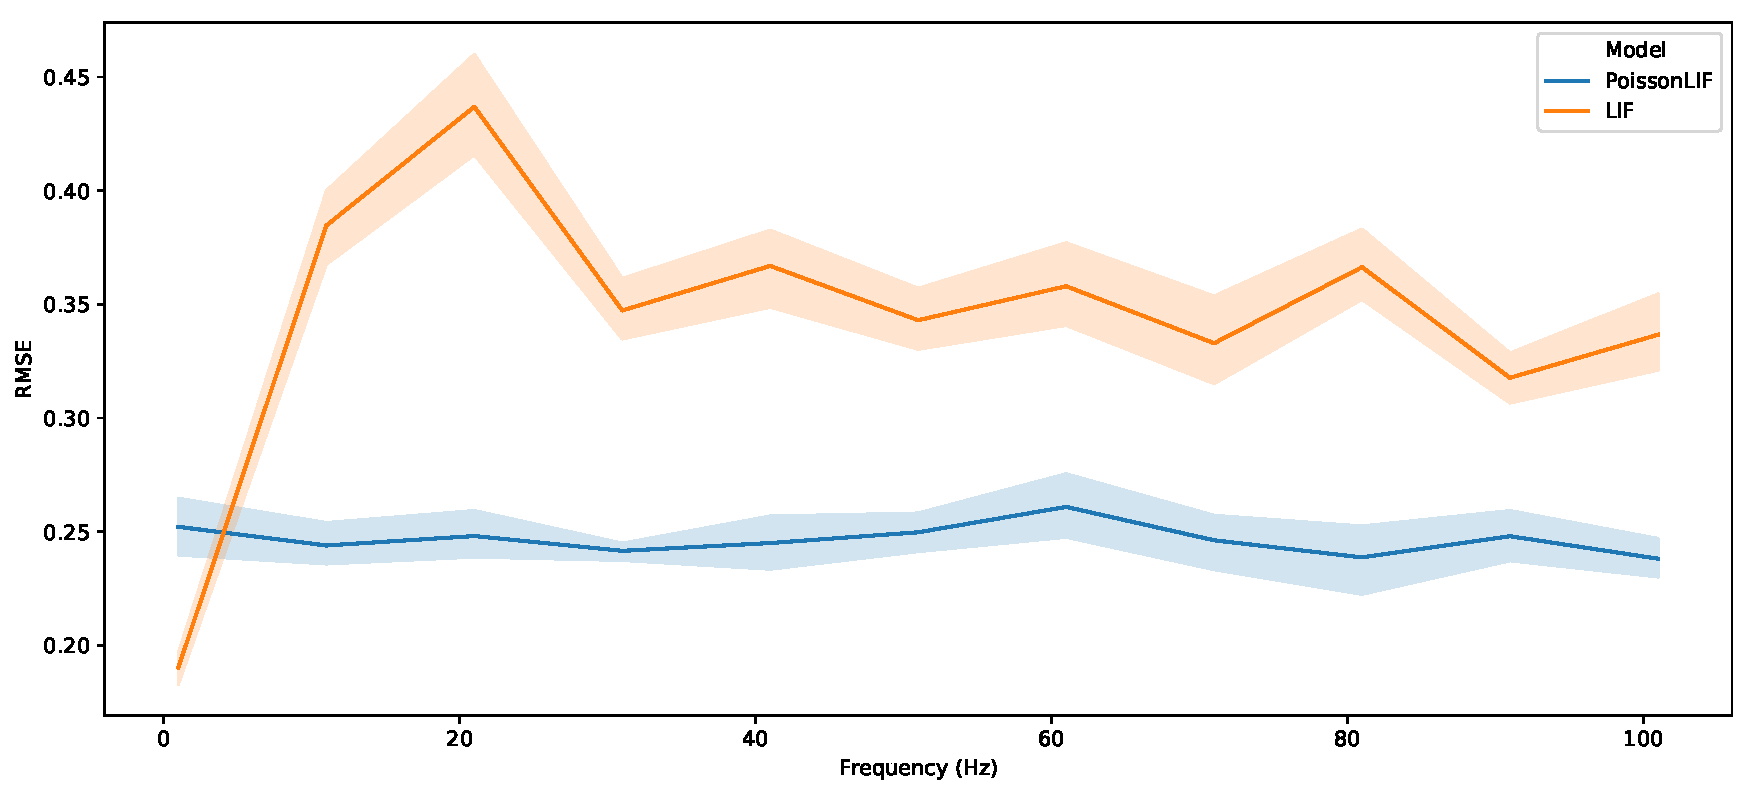
\includegraphics[width=0.9\textwidth]{poisson-frequency-scaling}
\caption[Spiking neuron performance with input frequency.]{\label{fig:poisson-frequency-scaling} Scaling of LIF performance with frequency, for each type: Poisson-spiking, non-leaky (i.e.,~integrate-and-fire), adaptive, and regular-spiking.
The input is a sinusoid with frequency $f$\,Hz.
% Both the ideal sinusoid and the decoded spike trains are filtered by $\tau = 0.01 f^{-1}$\,s to compute the RMSE.
%The number of neurons is set to $50 f$ in order to scale the total number of spikes with the input frequency, and the maximum firing rate of each neuron is uniformly distributed over $20-40$\,Hz.
%We give the LIF neurons an advantage by washing out the initial transient induced by an initial voltage of $v(0) = 0$.
Due to the memoryless property of the Poisson process, and the uniformity of ReLU, both outperform LIF with constant precision as $f \rightarrow \infty$ (Theorem~\ref{thm:correctness}), assuming $n$ and $\tau$ are scaled appropriately with frequency (see text for details).
}

\vspace{1em}

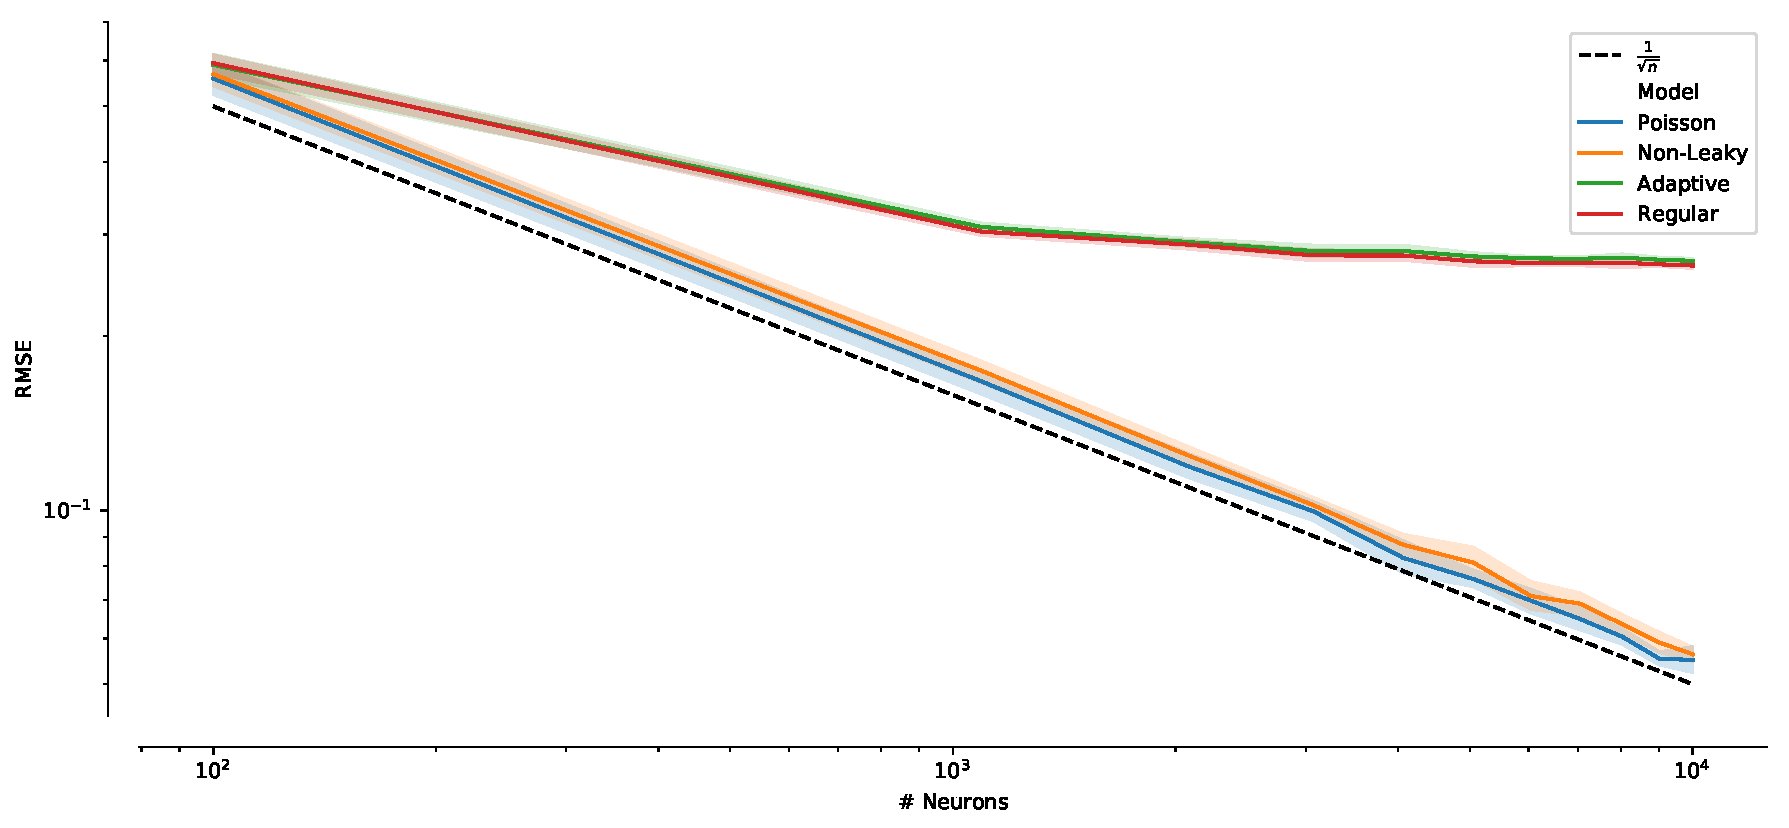
\includegraphics[width=0.9\textwidth]{poisson-neuron-scaling}
\caption[Spiking neuron performance with neuron count.]{\label{fig:poisson-neuron-scaling} Scaling of LIF performance with neuron count, for each type: Poisson-spiking, non-leaky (i.e.,~integrate-and-fire), adaptive, and regular-spiking.
%The input signal is a sinusoid with frequency $10$\,Hz, and the maximum firing rates are uniformly distributed over $20-40$\,Hz.
Regular-spiking LIF plateaus in performance for large numbers of neurons, due to the state discrepancy (definition~\ref{def:state-discrepancy}).
The precision of integrate-and-fire and Poisson-spiking both scale as ${\sqrt{n}}$ as $n \rightarrow \infty$ (Theorem~\ref{thm:correctness}), since each neuron is always ready to spike with the ideal probability. 
}
\end{figure}

We validate these claims in Figures~\ref{fig:poisson-frequency-scaling} and~\ref{fig:poisson-neuron-scaling} by using each type of LIF model---Poisson-spiking, non-leaky, adaptive, and regular-spiking---evaluating the root-mean-squared error (RMSE) against the filtered ideal.
In all cases the maximum firing rates of the neurons are limited to $20$--$40$\,Hz, and the states of the neurons are initialized to be mixed (i.e.,~uniform ISIPs).
In both figures we display 95\% confidence intervals bootstrapped from $10$ trials in each condition.

In Figure~\ref{fig:poisson-frequency-scaling}, we demonstrate that precision remains constant for both Poisson-spiking and non-leaky neurons, even at frequencies greater than six times that of the maximum firing rates of any given neuron.
For this, we set $n = 50 f$, $\tau = 10 f^{-1}$\,ms, and $\dt{} = 1 f^{-1}$\,ms, as we scale the frequency of the sinusoid, $f$\,Hz.
This choice of scaling is informed by equation~\ref{eq:psc-code-power}, which tells us that we should balance $\tau = f^{-1}$ to keep $\bigoh{2 \pi \tau f }$ fixed, while increasing $n$ in proportion to $f$ to scale the total number of spikes with frequency.
Due to the variability in a Poisson process, it is sub-optimal for constant inputs.
However, performance remains constant at higher frequencies.

In Figure~\ref{fig:poisson-neuron-scaling}, we demonstrate that the precision continues to scale as $\bigoh{\tau \sqrt{n}}$ for both Poisson-spiking and non-leaky neurons, but not for the other two.
For this, we fix $f = 10$\,Hz, $\tau = 1$\,ms, and $\dt{} = 0.1$\,ms, as we scale the neuron count.
This demonstrates that Posson spiking models (and ReLU) solve the state discrepancy problem, and thus continue to scale in accuracy with neuron count at increasingly-greater signal frequencies relative to the individual firing rates.
The properties of the Poisson neuron model make it particularly appealing for neuromorphic architectures such as SpiNNaker~2.
Specifically, SpiNNaker~2 has specialized hardware for computing exponentials~\citep{partzsch2017fixed} and uniform samples~\citep{liu2018memory}, and the architecture benefits enormously from the reduction of memory requirements and spike-traffic~\citep{stromatias2013power, mundy2015}.
Since the Poisson spike generator can be applied to any desired static response curve, this method can be applied to whatever is cheap to compute while still providing a suitable nonlinear basis for the desired transformation.


\chapter{Delay Networks}
\label{chapt:delays}

This chapter has been adapted from, while significantly extending, the work of \citet[][patent pending]{voelker2015computing, dynamicspatent, voelker2018}.

A particularly important dynamical system that has not been discussed before in the NEF literature is the pure \emph{continuous-time delay} line.
In order to implement such a system, one must represent a \emph{rolling window} of input history, or, in other words, one must \emph{buffer} the input signal into a memory that continuously slides alongside the current input.
In this chapter, we provide a novel derivation of an optimal low-dimensional linear approximation to a continuous-time delay, and then realize this \emph{Delay Network}~(DN) using the NEF in a recurrent spiking network.
We then investigate its computational properties, proving that the resulting network implements a well-defined nonlinear encoding of its input across the delay interval -- isomorphic to a high-dimensional projection of the Legendre polynomials.
This network uses a scale-invariant representation, with a level of accuracy that depends on the input frequency, chosen dimensionality (i.e.,~the order of the approximation), and particular synapse model.
To our knowledge, this work is the first to demonstrate that such a temporal code may be accurately implemented using a spiking dynamical network.

Reservoir Computing approaches, such as Liquid State Machines~\citep{maass2002real} and Echo State Networks~\citep{jaeger2001echo}, may be used to approximate a delay line.
However, since these networks use randomly chosen feedback weights, we show in section~\ref{sec:delay-rc} that they do so with relatively poor accuracy despite extensive hyper-optimization.
Such networks instead represent a random variety of nonlinear memory traces~\citep{lukovsevicius2012reservoir}.
Discrete approaches to short-term memory, such as those taken by \citet{white2004short} and \citet{ganguli2008memory}, while optimal in an information-theoretic sense, rely fundamentally on single time-step delays between rate-based neurons.
In contrast, the method that we propose here works independently of the simulation time-step, and is optimal assuming the population of spiking neurons---coupled with some model of the synapse---accurately represents a low-dimensional, low-frequency, vector space.
Furthermore, we use our extensions from section~\ref{sec:synaptic-extensions}, which improves our understanding of the relationship between synapse models and network-level computations.

We also find that the delay-line is a difficult function for FORCE networks to learn (section~\ref{sec:force-comparison}); re-encoding the delayed output as a teaching signal ends up ``confusing'' the network.
Furthermore, we find that our network, when expressed as an RNN cell (without spikes), outperforms equivalently-sized stacked LSTMs on computing long delays, and predicting the Mackey-Glass dataset---a difficult chaotic time-series benchmark---in training time, inference time, and test accuracy.
We then reveal some connections between the neural responses within our delay network, and ``time cells'' in the neuroscience literature.
Lastly, we discuss a number of theoretical applications that are directly supported by, and extend, the computations of the delay network.

To begin, consider a continuous-time delay line of $\theta$ seconds:
\begin{align} \label{eq:time-delay}
y(t) = (u \ast \delta_{\theta})(t) = u(t - \theta)\text{,} \quad \theta > 0 \text{,}
\end{align}
where $\delta_{\theta}$ denotes the Dirac delta shifted forwards in time by $\theta$.
This system takes a time-varying scalar signal, $u(t)$, and outputs a purely delayed version, $u(t - \theta)$.
The task of computing this function both accurately and efficiently in a biologically plausible, spiking, dynamical network, is a significant theoretical challenge, that, to our knowledge, has previously remained unsolved.

The continuous-time delay is worthy of detailed consideration for several reasons.
First, it is non-trivial to implement using continuous-time spiking dynamical primitives.
Specifically, equation~\ref{eq:time-delay} requires that we maintain a \emph{rolling window} of length $\theta$ (i.e.,~the history of $u(t)$, going $\theta$ seconds back in time).
Thus computing a delay of $\theta$ seconds is just as hard as computing every delay of length $\theta'$, for all $0 \le \theta' \le \theta$.
Since any finite interval of $\mathbb{R}$ contains an uncountably-infinite number of points, an exact solution for arbitrary $u(t)$ requires that we maintain an uncountably-infinite amount of information in memory.
Second, the delay provides us with a window of input history from which to compute arbitrary nonlinear functions across time.
For instance, the spectrogram of a signal may be computed by a nonlinear combination of delays, as may any finite impulse response~(FIR) filter.
Third, delays introduce a rich set of interesting dynamics into large-scale neural models, including: oscillatory bumps, traveling waves, lurching waves, standing waves, aperiodic regimes, and regimes of multistability~\citep{roxin2005role}.
Fourth, a delay line can be coupled with a single nonlinearity to construct a network displaying many of the same benefits as Reservoir Computing~\citep{appeltant2011information, bai2018dfr}.

Many learning algorithms also tend to rely on sliding windows of input history.
For instance, \citet{leng2013online} and \citet{izzeldin2011online} improved their neural networks' accuracy by incorporating sliding windows into their learning rules -- but they did not offer any neural implementation for the component that performs the required buffering.
Similarly, \citet{ferreira2009online} found sliding windows to be beneficial for the online learning of process models, in which the parameters of a nonlinear time-varying system are identified.

The computational power of delays is explained more abstractly by Takens' embedding theorem~\citep{takens1981detecting, noakes1991takens}.\footnote{%
We thank Peter Suma for pointing out this connection.
}
This theorem provides a very deep connection between delays and dynamical systems, specifically: any chaotic attractor, with finite box counting dimension, $k$, can be reconstructed by a static nonlinear projection of $2k$ different delays of just \emph{one} of its internal state variables.
In other words, a basis of delays, when applied to just a single observed variable, provides enough information to infer its entire unobserved state.
These insights have practical applications to time-series forecasting in the natural sciences~\citep{sugihara2012detecting}.
And, in particular, this provides theoretical grounding for why delays might be computationally useful in biological systems; their dynamics support the inference of high-dimensional states from low-dimensional observations over time.

Our delay network is also somewhat analogous to an autoencoder~\citep{gulli2017deep} from machine learning.
However, rather than compressing the input into a low-dimensional space that allows for it to be reconstructed spatially, we do this \emph{temporally}.
This leads to a number of applications that can, in effect, mentally travel back in time using just a handful of latent state-variables embedded within a spiking network.
The resulting representations are fully interoperable with the semantic pointer architecture~\citep[SPA;][]{eliasmith2012}, and thus afford the same manipulations as semantic pointers in Spaun, namely: binding into working memory, compressing information from cortex, internally routing information, and driving motor actions~\citep{eliasmith2013build}.

At a higher level, any physical realization of a delay must necessarily be modelling the statistics of its input in some way.
This is because it is physically impossible to buffer arbitrary signals in continuous time (details in section~\ref{sec:nef-delay}), and thus some sacrifice must be made.
In essence, this sacrifice amounts to a sparse coding mechanism, in which a low-dimensional representation is constructed that maps onto the infinite-dimensional time window~\citep{blumensath2009sampling}.
Spikes in a neural network are akin to such a compression mechanism in time, as are decoders in space.
Our solution leverages both methods of sparsification, but not in a way that one might come to expect from information theory or other approaches involving discrete samples; our NEF-based approach finds the optimal system for linearly mapping continuous-time windows onto a low-dimensional manifold.

\section{Derivations}
\label{sec:derivations}

It is impossible in practice (i.e.,~given finite-order continuous-time resources) to implement an arbitrary delay.
For instance, a white noise signal contains an uncountably-infinite amount of information within any finite window, that cannot be compressed any further~\citep{cover2012elements}.
We instead approximate $u(t)$ as a low-frequency signal, or, equivalently, approximate equation~\ref{eq:time-delay} as a low-dimensional system expanded about the zeroth frequency in the \emph{Laplace domain}.
Our choice of a zero-frequency approximation is informed by our analysis from section~\ref{sec:energy-minimization}, which suggests that neural systems require energy that grows linearly in the representational frequency.

\subsection{Optimal approximation}
\label{sec:nef-delay}

% However, different approximations at this stage would allow for more efficient coding of particular statistics.
We begin by transforming equation~\ref{eq:time-delay} into the Laplace domain, $\mathcal{L} \left\{ y(t) \right\} = \mathcal{L} \left\{ u(t) \right\} \mathcal{L} \left\{ \delta_{\theta}(t) \right\}$, and then using the fact that $\mathcal{L} \left\{ \delta_{\theta}(t) \right\} = e^{-\theta s}$ to obtain:
\begin{align} \label{eq:tf-delay}
F(s) := \frac{\mathcal{L} \left\{ y(t) \right\}}{\mathcal{L} \left\{ u(t) \right\}} = e^{-\theta s} \text{,}
\end{align}
where $F(s)$ is known as the \emph{transfer function} of the system, defined as the ratio of the Laplace transform of the output to the Laplace transform of the input.
Equation~\ref{eq:tf-delay} should be understood as an equivalent way of expressing equation~\ref{eq:time-delay} in the Laplace domain, where the variable $s$ denotes a complex frequency. 
Notably, we have not made any sacrifices at this point, as the ideal system is a linear dynamical system.
Thus far, we have only described the transfer function that we would like the network to implement. %while $t$ is non-negative in the time domain.
% Unimportant reminder? The transfer function is the Laplace transform of system's impulse response.

The state-space model discussed in section~\ref{sec:principle3} (equation~\ref{eq:lti}) is related to its transfer function by equation~\ref{eq:ss2tf}.
Conversely, a transfer function can be converted into a state-space model satisfying equation~\ref{eq:ss2tf} \emph{if and only if} it can be written as a proper ratio of finite polynomials in $s$~\citep{brogan1982modern}.
The ratio is proper when the degree of the numerator does not exceed that of the denominator.
In such a case, the output will not depend on future input, and so the system is \emph{causal}.
The degree of the denominator corresponds to the dimensionality of the state-vector, and therefore must be finite.
These two conditions align with physically realistic constraints where time may only progress forward, and neural resources are limited.

However, the pure delay (equation~\ref{eq:tf-delay}) has infinite order when expressed as a ratio of polynomials in $s$, and so the system is irrational, or infinite-dimensional.
Consequently, no finite state-space model will exist for $F(s)$, which formalizes our previous remark that an exact solution is impossible for finite, continuous-time systems.
To overcome this, we must approximate the irrational transfer function $e^{-\theta s}$ as a proper ratio of finite-order polynomials.
We do so using its \emph{Pad\'e approximants}---the coefficients of a Taylor series extended to the ratio of two polynomials---expanded about $s=0$~\citep{Pade1892, vajta2000some}:
\begin{equation} \label{eq:pade}
\begin{aligned}
\left[ p/q \right] e^{-\theta s} &= \frac{\mathcal{B}_{p}(-\theta s)}{\mathcal{B}_{q}(\theta s)} \text{,} \\
\quad \mathcal{B}_m(s) &:= \sum_{i=0}^m \begin{pmatrix}m \\ i\end{pmatrix} \frac{(p + q - i)!}{(p + q)!} s^i \text{.}
\end{aligned}
\end{equation}
This provides the transfer function of order $p$ in the numerator and order $q$ in the denominator that optimally approximates equation~\ref{eq:tf-delay} for low-frequency inputs (i.e.,~up to order $p + q$).

After choosing $0 \le p \le q$, we may numerically find a state-space model $(A\text{,}\, B\text{,}\, C\text{,}\, D)$ that satisfies equation~\ref{eq:ss2tf} using standard methods,\footnote{%
For instance, the function \texttt{tf2ss} in MATLAB or SciPy.}
and then map this system onto the synapse using Principle~3.
%This works independently of the chosen simulation time-step using equation~\ref{eq:p3discrete}.
However, na\"ively applying this conversion leads to numerical issues in the representation (i.e.,~dimensions that grow exponentially in magnitude), due in part to the factorials in equation~\ref{eq:pade}.

To overcome this problem, we derive an equivalent yet normalized state-space model that we have not encountered elsewhere.
We do so for the case of $p = q - 1$, since this provides the best approximation to the step-response. We symbolically transform equation~\ref{eq:pade} into a normalized state-space model that avoids the need to compute any factorials.
We first do so for the special case of $p = q - 1$, since this provides the best approximation to the step-response~\citep{vajta2000some}.
We begin by expanding equation~\ref{eq:pade}:
\begin{align*}
[q-1/q]e^{-\theta s} &= \frac{\sum_{i=0}^{q-1} \begin{pmatrix}{q-1} \\ i\end{pmatrix} (2q - 1 - i)! (-1)^i \theta^i s^i}{\sum_{i=0}^q \begin{pmatrix}q \\ i\end{pmatrix} (2q - 1 - i)! \theta^i s^i} \\
&= \frac{\frac{1}{\theta^{q} (q-1)!} \sum_{i=0}^{q-1} \frac{(q-1)!}{(q-1-i)!i!} (2q - 1- i)! \theta^i s^i (-1)^i}{s^q + \frac{1}{\theta^q (q-1)!}  \sum_{i=0}^{q-1} \frac{q!}{(q-i)!i!} (2q - 1 - i)! \theta^i s^i} \\
&= \frac{\sum_{i=0}^{q-1} c_i s^i}{s^q + \sum_{i=0}^{q-1} d_i s^i} \text{,}
\end{align*}
where $d_i := \frac{q(2q - 1 - i)!}{(q-i)!i!} \theta^{i-q}$ and $c_i := (-1)^i \left( \frac{q-i}{q} \right) d_i$.

This transfer function is readily converted into a state-space model in controllable canonical form:
\begin{equation*}
    \begin{alignedat}{2}
        A &= \begin{pmatrix} -d_{q-1} & -d_{q-2} & \cdots & -d_0 \\ 1 & 0 & \cdots & 0 \\ 0 & \ddots & \ddots & \vdots \\ 0 & 0 & 1 & 0\end{pmatrix} \text{,} & & \quad\quad \begin{alignedat}{1}
            B &= \transpose{\begin{pmatrix} 1 & 0 & \cdots & 0\end{pmatrix}} \text{,} \\
            C &= \begin{pmatrix} c_{q-1} & c_{q-2} & \cdots & c_0\end{pmatrix} \text{,} \\
            D &= 0 \text{.}
        \end{alignedat}
    \end{alignedat}
\end{equation*}
To eliminate the factorials in $d_i$ and $c_i$, we scale the $i^{\text{th}}$ dimension of the state-vector by $d_{q-1-i}$, for all $i = 0 \ldots q - 1$.
This is achieved without changing the transfer function by scaling each $(B)_j$ by $d_{q-1-j}$, each $(C)_i$ by $1 / d_{q-1-i}$, and each $(A)_{ij}$ by $d_{q-1-i} / d_{q-1-j}$, which yields the equivalent state-space model:
\begin{equation}
    \begin{alignedat}{2}
        A &= \begin{pmatrix} -v_0 & -v_0 & \cdots & -v_0 \\ v_1 & 0 & \cdots & 0 \\ 0 & \ddots & \ddots & \vdots \\ 0 & 0 & v_{q-1} & 0\end{pmatrix} \text{,} & & \quad\quad \begin{alignedat}{1}
            B &= \transpose{\begin{pmatrix} v_0 & 0 & \cdots & 0\end{pmatrix}} \text{,} \\
            C &= \begin{pmatrix} w_0 & w_1 & \cdots & w_{q-1} \end{pmatrix} \text{,} \\
            D &= 0 \text{,} \label{eq:ss-delay}
        \end{alignedat}
    \end{alignedat}
\end{equation}
where $v_i := \frac{(q+i)(q-i)}{i+1} \theta^{-1}$ and $w_i := (-1)^{q - 1 - i} \left( \frac{i+1}{q} \right)$, for $i = 0 \ldots q-1$.
This follows from noting that $v_0 = d_{q-1}$ and $v_i := d_{q-1-i} / d_{q-i}$ for $i \ge 1$.

A similar derivation applies to the case where $p = q$, although it results in a passthrough ($D \ne 0$) which is suboptimal for step-responses.
For brevity, we omit this derivation, and instead simply state the result:
\begin{equation*}
    \begin{alignedat}{2}
        A &= \begin{pmatrix} -v_0 & -v_0 & \cdots & -v_0 \\ v_1 & 0 & \cdots & 0 \\ 0 & \ddots & \ddots & \vdots \\ 0 & 0 & v_{q-1} & 0\end{pmatrix} \text{,} & & \quad\quad \begin{alignedat}{1}
            B &= \transpose{\begin{pmatrix}-v_0 & 0 & \cdots & 0\end{pmatrix}} \text{,} \\
            C &= \begin{pmatrix} 2(-1)^q & 0 & 2(-1)^q & 0 & \cdots & \cdots \end{pmatrix} \text{,} \\
            D &= (-1)^q \text{,}
        \end{alignedat}
    \end{alignedat}
\end{equation*}
where $v_i = \frac{(q+i+1)(q-i)}{i+1} \theta^{-1}$, for $i = 0 \ldots q-1$.

In either case, $A$ and $B$ depend on the delay length solely by the scalar factor $\theta^{-1}$.
For this reason, and to keep quantities dimensionless, we often make the substitution $\V{x}(t) \leftarrow \theta\V{x}(t)$ to express the system in an alternative form~\citep{braindrop2019}:
\begin{equation} \label{eq:delay-system}
  \theta \dot{\V{x}}(t) = A\V{x}(t) + Bu(t) \text{,} \quad
  A = \begin{pmatrix} -v_0 & -v_0 & \cdots & -v_0 \\ v_1 & 0 & \cdots & 0 \\ 0 & \ddots & \ddots & \vdots \\ 0 & 0 & v_{d-1} & 0\end{pmatrix} \text{,} \quad 
  B = \transpose{\begin{pmatrix} v_0 & 0 & \cdots & 0\end{pmatrix}} \text{,} 
\end{equation}
where $v_i := (q+i)(q-i)(i+1)^{-1}$ no longer depends on $\theta$. %and $w_i := (-1)^{d - 1 - i} \left( \frac{i+1}{d} \right)$
As a side-effect, we may \emph{control} the length of the delay by adjusting the gain on the integration time-constant (i.e.,~by scaling the input and feedback signals).
The NEF can be used to build such controlled dynamical systems, without introducing multiplicative dendritic interactions or implausible on-the-fly connection weight scaling~\citep{eliasmith2000b}.

This model is now equivalent to equation~\ref{eq:pade}, but without any factorials, and in the form of equation~\ref{eq:lti}.\footnote{%
In section~\ref{sec:software}, we mention NengoLib's features for several other state-space realizations.}
The choice of $q$ corresponds to the dimensionality of the latent state-vector $\V{x}(t)$ that is to be represented by Principle~1 and transformed by Principle~2.
Principle~3 may then be used to map equation~\ref{eq:ss-delay} onto a spiking dynamical network to accurately implement an optimal low-frequency approximation of the delay.

To demonstrate, we implement a $1$\,s delay of $1\,$Hz band-limited white noise using $\numprint{1000}$ recurrently connected spiking LIF neurons representing a $6$-dimensional vector space (see Figure~\ref{fig:delay-example}).
The connections between neurons are determined by applying Principle~3 (section~\ref{sec:principle3}) to the state-space model derived above (equation~\ref{eq:ss-delay}, $q=6$) via the Pad\'e approximants of the delay.
The normalized root-mean-squared error (NRMSE; normalized so that $1.0$ would correspond to random chance) of the output signal is $4.8$\%.
This is achieved without appealing to the simulation time-step ($\dt{} = 1$\,ms); in fact, as shown in section~\ref{sec:pure_delay}, the network accuracy improves as $\dt{}$ approaches zero due to the continuous-time assumption mentioned in section~\ref{sec:principle3} (and relaxed in section~\ref{sec:linear-extensions}).

\begin{figure}
  \centering
  \includegraphics[width=\textwidth]{{NECO-04-17-2838-Figure.3}.pdf}
  \caption[Example simulation of a spiking Delay Network.]{ \label{fig:delay-example}
    Delay of $1$\,s implemented by applying standard Principle~3 to equation~\ref{eq:ss-delay} using $q = 6$, $\dt{}=1$\,ms, $\numprint{1000}$ spiking LIF neurons, and a lowpass synapse with $\tau=0.1$\,s.
    The input signal is white noise with a cutoff frequency of $1$\,Hz.
    The plotted spikes are filtered with the same $\tau=0.1$\,s, and encoded with respect to $\numprint{1000}$ encoders sampled uniformly from the surface of the hypersphere (sorted by time to peak activation).
    Reproduced from \citet[][Figure~3]{voelker2018}.
  }
\end{figure}

\subsection{Temporal representation}
\label{sec:temporal-representation}

Although the delay network has its dynamics optimized for a single delay $\theta > 0$, we may still accurately decode any delay $0 \le \theta' \le \theta$ from the state of the same network, as intuitively it needs to be holding onto this memory.
In other words, the network is representing a rolling window (i.e.,~history) of length $\theta$.
To compute these other delays, we must approximate $e^{-\theta' s}$ with a transfer function
$$F_{\theta \rightarrow \theta'}(s) := \frac{\mathcal{C}(s; \, \theta, \theta')}{\mathcal{D}(s; \, \theta)}$$
of order $[p / q]$, such that the denominator $\mathcal{D}(s; \, \theta)$ (which provides us with the recurrent transformation up to a change of basis) depends only on $\theta$, while the numerator $\mathcal{C}(s; \, \theta, \theta')$ (which provides us with the output transformation up to a change of basis) depends on some relationship between $\theta'$ and $\theta$.

From equation~\ref{eq:pade}, we may write the denominator as:
\begin{align*}
\mathcal{D}(s; \, \theta) = \sum_{i=0}^q d_i(\theta) s^i \text{,} \quad d_i(\theta) := \begin{pmatrix}q \\ i\end{pmatrix} \frac{(p + q - i)!}{(p + q)!} \theta^i \text{.}
\end{align*}
We then solve for the numerator, as follows:
\begin{align*}
&& [p/q] e^{-\theta' s} &= \sum_{i=0}^\infty \frac{(-\theta' s)^i}{i !} = \frac{\mathcal{C}(s; \, \theta, \theta')}{\mathcal{D}(s; \, \theta)} & \\
&& \iff \quad \mathcal{C}(s; \, \theta, \theta') &= \left( \sum_{i=0}^\infty \frac{(-\theta' s)^i}{i !} \right) \left( \sum_{j=0}^q d_j(\theta) s^j \right) + \bigoh{s^{p + 1}} \text{.}
\end{align*}
By expanding this product and collecting like terms, the correct numerator up to order $p \le q$ is:
\begin{align*}
\mathcal{C}(s; \, \theta, \theta') = \sum_{i=0}^p c_i(\theta, \theta') s^i \text{,} \quad c_i(\theta, \theta') :=  \sum_{j=0}^i \frac{(- \theta')^{i - j}}{(i - j)!} d_j(\theta) \text{.}
\end{align*}
Therefore, the optimal readout for a delay of length $\theta'$, given the dynamics for a delay of length $\theta$, is determined by the above linear transformation of the coefficients $\left( d_j(\theta) \right)_{j=0}^p$.

We remark that $c_i(\theta, \theta) = \begin{pmatrix}p \\ i\end{pmatrix} \frac{(p + q - i)!}{(p + q)!} (-\theta)^i$, since $F_{\theta \rightarrow \theta}(s) = [p/q] e^{-\theta s}$, by uniqueness of the Pad\'e approximants, and by equation~\ref{eq:pade}.
As a corollary, we have proven that the following combinatorial identity holds for all $p, q \in \mathbb{N}$ and $i \in \left[ 0, \min\{p, q\} \right]$:
\begin{align*}
\begin{pmatrix}p \\ i\end{pmatrix} = \sum_{j=0}^i (-1)^j \begin{pmatrix}q \\ j\end{pmatrix} \begin{pmatrix}p + q - j \\ i - j\end{pmatrix} \text{.}
\end{align*}

For the case when $p = q - 1$, we may also apply the same state-space transformation used to derive equation~\ref{eq:ss-delay} to obtain the normalized coefficients for the $C$ transformation (i.e.,~with $A$, $B$, and $D$ unchanged):
\begin{align*}
w_{q-1-i} &= \left( \sum_{j=0}^i \frac{(-\theta')^{i-j}}{(i - j)!} \begin{pmatrix}q \\ j\end{pmatrix} \frac{(2q - 1 - j)!}{(2q - 1)!} \theta^j \right) \left( \frac{(q - i)! i! (2q - 1)!}{\theta^q (q - 1)! q(2q - 1 - i)!} \theta^{q - i} \right) \\
&= \sum_{j=0}^i \begin{pmatrix}q \\ j\end{pmatrix} \left( \frac{(2q - 1 - j)!}{(i - j)! (2q - 1 - i)!} \right) \left( \frac{(q - i)! i!}{q!} \right) \left( \theta^{j - i} \right) (-\theta')^{i - j} \\
&= \begin{pmatrix}q \\ i\end{pmatrix}^{-1} \sum_{j=0}^i \begin{pmatrix}q \\ j\end{pmatrix} \begin{pmatrix}2q - 1 - j \\ i - j\end{pmatrix} \left( \frac{-\theta'}{\theta} \right)^{i - j} \text{,} \quad i = 0 \ldots q - 1 \text{.}
\end{align*}
From this, we see that different decodings require different linear output transformations ($C$) for each $\theta'$, with the following coefficients:
\begin{align} \label{eq:delay-readouts}
w_{q-1-i} = \begin{pmatrix}q \\ i\end{pmatrix}^{-1} \sum_{j=0}^i \begin{pmatrix}q \\ j\end{pmatrix} \begin{pmatrix}2q - 1 - j \\ i - j\end{pmatrix} \left( \frac{-\theta'}{\theta} \right)^{i - j} \text{,} \quad i = 0 \ldots q - 1 \text{.} 
\end{align}
The underlying dynamical state remains the same.
To be clear, the $q$-dimensional state-vector of the delay network represents a rolling window of length $\theta$.
That is, a single delay network with some fixed $\theta > 0$ may be used to accurately decode any delay of length $\theta'$ ($0 \le \theta' \le \theta$) by taking a linear transformation of its state-vector according to the coefficients of equation~\ref{eq:delay-readouts}.

% Apart from providing a means of understanding the state-vector, the basis functions from equation~\ref{eq:delay-readouts} also provide a number of ways to readily exploit the delay network.
% a) differentiate any point up to q times
% b) "preferred window" of each neuron
% c) projecting the window function onto state-space
% d) characterizing the possible functions using Principles 1+2 and the inverse basis functions

In Figure~\ref{fig:delay-full}, we take different linear transformations of the same state-vector, by evaluating equation~\ref{eq:delay-readouts} at various delays between $0$ and $\theta$, to decode the rolling window of input from the state of the system.\footnote{%
The optimization problem from equation~\ref{eq:decoder_solution} need only be solved once to decode $\V{x}(t)$ from the neural activity.
The same decoders may then be transformed by each $C$ without loss in optimality (by linearity).
}
This demonstrates that the delay network compresses the input's history (lasting $\theta$ seconds) into a low-dimensional state.
\begin{figure}
  \centering
  \includegraphics[width=\textwidth]{{NECO-04-17-2838-Figure.4}.pdf}
  \caption[Accuracy of the Delay Network across its window.]{ \label{fig:delay-full}
    Decoding a rolling window of length $\theta$.
    Each line corresponds to a different delay, ranging from $0$ to $\theta$, decoded from a single delay network ($q = 12$).
    (Left)~Error of each delay, as the input frequency, $f$, is increased relative to $\theta$.
    Shorter delays are decoded more accurately than longer delays at higher frequencies.
    A triangle marks $\theta = f^{-1}$.
    (Right)~Example simulation decoding a rolling window of white noise with a cutoff frequency of $\theta^{-1}$\,Hz.
    Reproduced from \citet[][Figure~4]{voelker2018}.
    % See appendix~\ref{app:window} for details.
  }
\end{figure}
In Figure~\ref{fig:basis-functions}, we sweep equation~\ref{eq:delay-readouts} across $\theta' \theta^{-1}$ to visualize the temporal ``basis functions'' of the delay network.
This provides a means of understanding the relationship between the chosen state-space representation (i.e.,~the $q$-dimensional $\V{x}(t)$) and the underlying window representation (i.e.,~the infinite-dimensional $u(t)$).
In particular, each basis function corresponds to the continuous window of history represented by a single dimension of the delay network.
The instantaneous value of each dimension acts as a coefficient on its basis function, to contribute to the representation of the window at that point in time.
Overall, the entire state-vector determines a linear combination of these $q$ basis functions to represent the window.
An intriguing consequence of this and equation~\ref{eq:delay-readouts}, is that the temporal code employed by this network---in terms of the basis functions that it takes to reconstruct the window---is a linear transformation of the \emph{shifted Legendre polynomials}, $\mathcal{P}_i\left(2 \left(\theta' \theta^{-1}\right) - 1\right)$ up to the same order ($i = 0 \ldots q - 1$), with previous connections having been made between these same polynomials and parameter identification in time-delay systems~\citep{hwang1985analysis}. 
This means the network effectively projects the input onto its Legendre basis over time, thus providing a low-dimensional polynomial representation with coefficients given by the state-vector.
% This is analogous to the static function representation explored previously within the context of Principles~1 and~2~\citep[][pp.~63--72]{eliasmith2003a}.

\begin{figure}
  \centering
  \includegraphics[width=\textwidth]{{NECO-04-17-2838-Figure.5}.pdf}
  \caption[Temporal representation of the Delay Network.]{ \label{fig:basis-functions}
    Temporal basis functions of the delay network ($q = 12$).
    Each line corresponds to the basis function of a single dimension~($i$) ranging from $0$~(darkest) to $q - 1$~(lightest).
    The $i^\text{th}$ basis function is a polynomial over $\theta' \theta^{-1}$ with degree $i$ (see equation~\ref{eq:delay-readouts}). % ($0 \le \theta' \le \theta$).
    The state-vector of the delay network takes a linear combination of these $q$ basis functions in order to represent a rolling window of length $\theta$.
    Reproduced from \citet[][Figure~5]{voelker2018}.
  }
\end{figure}

The encoder of each neuron can also be understood directly in these terms as taking a linear combination of the basis functions (via equation~\ref{eq:encoding}).
Each neuron nonlinearly encodes a projection of the rolling window onto some ``preferred window'' determined by its own encoder.
Since the state-vector is encoded by heterogeneous neural nonlinearities, the population's spiking activity supports the decoding of nonlinear functions across the entire window (i.e.,~functions that we can compute using Principles~1 and~2).
Therefore, we may conceptualize the delay network as a \emph{temporal coding} of the input stimulus, which constructs a low-dimensional state---representing an entire window of history---to encode the temporal structure of the stimulus into a nonlinear high-dimensional space of neural activities.
We discuss this in more detail in the following section.

To more thoroughly characterize the delay dynamics, we analyze the behavior of the delay network as the dimensionality is increased (see Figure~\ref{fig:pca}).
Specifically, we perform a standard principal component analysis~(PCA) on the state-vector for the impulse response, and vary the order from $q=3$ to $q=27$.
This allows us to visualize a subset of the state-vector trajectories, via projection onto their first three principal components (see Figure~\ref{fig:pca}~(Top)). %\footnote{%
%These same trajectories are obtained by a PCA on the %filtered neural activities, by linearity of decoding.
%}
The length of this trajectory over time distinguishes different values of $q$ (see Figure~\ref{fig:pca}~(Bottom)).
This length-curve is approximately logarithmic when $q = 6$, convex when $q \le 12$, and sigmoidal when $q > 12$. % (also see Figure~\ref{fig:time-cells}~(Bottom)).
To generate this figure we use a delay of $\theta = 10\,$s, but in fact this analysis is scale-invariant with time.
This means that other delays will simply stretch or compress the impulse response linearly in time (not shown).

\begin{figure}
  \centering
  \includegraphics[width=\textwidth]{{NECO-04-17-2838-Figure.6}.pdf}
  \caption[State-space trajectories of the Delay Network.]{ \label{fig:pca}
    Impulse response of the delay network with various orders ($q$) of Pad\'e approximants.
    (Top)~The state-vector $\V{x}(t)$ projected onto its first three principal components.
    (Bottom)~The length of the curve $\V{x}$ up to time $t$, computed using the integral $\smallint \|\dot{\V{x}}(t)\|$ (normalized to $1$ at $t = \theta$).
    This corresponds to the distance travelled by the state-vector over time.
    The dashed line marks the last inflection point, indicating when $\V{x}(t)$ begins to slow down.
    % The slope of $d(t)$ is correlated with the number of neurons encoding $\V{x}(t)$ at time $t$, when using a random encoding (not shown).
    Reproduced from \citet[][Figure~6]{voelker2018}.
  }
\end{figure}

We remark that the delay network is scale-invariant with the delay length over input frequency, that is, the accuracy for a chosen order is a function of $f \times \theta$ (see units in Figure~\ref{fig:delay-full} for instance), where $f$ is the input frequency. % and the synaptic time-constants are scaled by $\theta$.
More specifically, for a fixed approximation error, the delay length scales as $\bigoh{ qf^{-1} }$.
We elaborate on these properties in section~\ref{sec:delay-scalability}, and demonstrate our extensions to harnessing arbitrary linear synapse models to improve accuracy in section~\ref{sec:pure_delay}.

\subsection{Nonlinear characterization}
\label{sec:delay-nonlinear}

A delay is a linear dynamical system.
However, by virtue of encoding the delay network's state-vector into a heterogeneous population of neurons---as in the first two principles of the NEF---the network also affords the computation of arbitrary nonlinear functions across the rolling window.
Recall that a continuous-time rolling window of length $\theta > 0$, which here we denote as $\left[ u(t - \theta') \,:\, 0 \le \theta' \le \theta \right]$, $u(\cdot) \in \mathbb{R}$, may be \emph{temporally compressed} into a low-dimensional state $\V{x}(t) \in \mathbb{R}^q$, by the following linear time-invariant dynamical system that approximately delays an input signal by $\theta$ seconds (repeating equation~\ref{eq:delay-system}, for clarity):
\begin{equation*}
  \theta \dot{\V{x}}(t) = A\V{x}(t) + Bu(t) \text{,} \quad
  A = \begin{pmatrix} -v_0 & -v_0 & \cdots & -v_0 \\ v_1 & 0 & \cdots & 0 \\ 0 & \ddots & \ddots & \vdots \\ 0 & 0 & v_{d-1} & 0\end{pmatrix} \text{,} \quad 
  B = \transpose{\begin{pmatrix} v_0 & 0 & \cdots & 0\end{pmatrix}} \text{,} 
\end{equation*}
where $v_i := (q+i)(q-i)(i+1)^{-1}$, %and $w_i := (-1)^{d - 1 - i} \left( \frac{i+1}{d} \right)$
for $i = 0 \ldots q-1$.
%We may also solve this system to express $\V{x}(t)$ as a convolution of $u$ with the SIMO impulse response $\V{f}$: 
%\begin{equation} \label{eq:lti-solved}
%\V{f}(t) = e^{At} B \text{,} \quad \V{x}(t) = \left(u \ast \V{f}\right)(t) \text{.}
%\end{equation}
This compression is derived by applying Pad\'e approximants to $e^{-\theta s}$ about the complex point $s=0$, which yields an optimal low-degree polynomial expansion of $\mathcal{L}\{u\}(s)$ about its zeroth frequency.
%\footnote{Note that a LTI system is equivalent up to any invertible linear transformation applied to the state-space.}
The state $\V{x}(t)$ represents the rolling window via a linear combination of time-invariant polynomial basis functions:
\begin{equation} \label{eq:basis-interpretation}
\boxed{u(t - \theta') \approx \sum_{i=0}^{q-1} \mathcal{P}_{i,q} \left(\frac{\theta'}{\theta} \right) \, x_{q-1-i}(t) \text{,} \quad 0 \le \theta' \le \theta \text{.} }
\end{equation}
Repeating the equation for these polynomials (equation~\ref{eq:delay-readouts}), for completeness:
\begin{equation} \label{eq:basis-functions}
\mathcal{P}_{i,q}(r) = \begin{pmatrix}q \\ i\end{pmatrix}^{-1} \sum_{j=0}^i \begin{pmatrix}q \\ j\end{pmatrix} \begin{pmatrix}2q - 1 - j \\ i - j\end{pmatrix} \left( -r \right)^{i - j} \text{.} %\text{,}\quad 0 \le r \le 1 \text{,}\quad i = 0 \ldots d - 1
\end{equation}
A set of polynomials $\{ \mathcal{P} \}_{i, q}$ are shown in Figure~\ref{fig:basis-functions}.
This means the system is implicitly projecting its window of history onto a linear transformation of the shifted Legendre basis functions.
In essence, equation~\ref{eq:basis-interpretation} determines a linear map from the $q$-dimensional state, $\V{x}(t)$, to the infinite-dimensional rolling window, $[ u(t - \theta') \,:\, 0 \le \theta' \le \theta ]$.
In other words, equation~\ref{eq:basis-interpretation} is the optimal pseudo-inverse of the linear compression defined by equation~\ref{eq:delay-system}.
%The frequencies in $u(t)$ that may be accurately encoded by this approach scale inversely with $\theta$.
%Likewise, higher values of $q$ allowed for higher frequencies to be encoded at the same level of precision.
%We remark that each basis function is expressed in terms of the unitless quantity $\frac{\theta'}{\theta}$, and is therefore scale-invariant.
%We may also transform the state by any invertible matrix (e.g.,~ to orthogonalize the basis functions) without loss of generality.
%Analysis of the approximation error, and some additional properties of this ``delay network'', may be found in \cite{voelker2018}.

Moreover, every point along the window, along with its Taylor series expansion up to order $q-1$, as well as any other linear operations across the rolling window (e.g.,~Laplace transform), may be expressed using equation~\ref{eq:basis-interpretation} and equation~\ref{eq:basis-functions} as a fixed, known dot product with $\V{x}(t)$.
To make this evident, let $k(\theta')$ ($0 \le \theta' \le \theta$) be any desired kernel (e.g.,~Fourier transform), then:
\begin{equation} \label{eq:delay-linear-transform}
\begin{aligned}
(u \ast k)(t) &= \int_{\theta'=0}^{\theta} u(t - \theta') k(\theta') \, d\theta' \\
&\approx \sum_{i=0}^{q-1} \underbrace{\left( \int_{\theta'=0}^{\theta} k(\theta') \mathcal{P}_{i,q} \left(\frac{\theta'}{\theta} \right) d\theta' \right)}_{k_{q -1-i}} x_{q-1-i}(t) \\
&= \left\langle \V{x}(t)\text{,}\, \V{k} \right\rangle \text{,}
\end{aligned}
\end{equation}
where $\V{k} = \transpose{\left[ k_0\text{,}\, \ldots \text{,}\, k_{q-1} \right]} \in \mathbb{R}^q$ is defined above independently of time.
Hence, any integral transform is simply a dot product with $\V{x}(t)$.
Similarly, one may obtain Taylor expansions by taking dot products with vectors derived by repeatedly differentiating both sides of equation~\ref{eq:basis-interpretation} with respect to $\theta'$ (not shown).
Crucially, such dot products are precisely what the encoders $\V{e}_i$ compute in equation~\ref{eq:encoding}.
This implies that the PSC of any neuron, by itself, necessarily represents a particular convolution across the window.\footnote{%
There are infinitely many, since the system is overcomplete when working backwards from $\V{k} \mapsto k(\cdot)$, but we can enforce uniqueness by imposing L2-regularization, for instance.}
The nonlinearity of each neuron thus provides a nonlinear function of some finite-width filter (Principle~1).
%Yet, as shown below, this does not restrict our ability to also perform nonlinear computations across the window.
More generally, the state $\V{x}(t)$ is \emph{encoded} by a heterogeneous population of neurons, which allows for arbitrary nonlinear functions across the window,
$$y(t) = f(\V{x}(t)) \approx f\left(\left[ u(t - \theta') \,:\, 0 \le \theta' \le \theta \right]\right)$$
to be \emph{decoded} from its activity (Principle~2).
For example, Figure~\ref{fig:delay-autocorrelation} visualizes $f$ within the space of $\V{x} \in \mathbb{R}^3$ for the autocorrelation function, $y(t) = u(t - \theta)\, u(t)$.

\fig{delay-autocorrelation}{0.5}{Autocorrelation function mapped onto the Delay Network.}{
  Visualizing the autocorrelation function $y(t) = u(t - \theta)\, u(t)$ with $q=3$.
  Each point along the surface of the unit-sphere is $\V{x}(t)$, and is coloured according to its corresponding value of $y(t)$ obtained from equation~\ref{eq:basis-interpretation}.
  A slice of the shell is cut away for visualization.
} 

\subsection{Scalability considerations}
\label{sec:delay-scalability}

\fig{pade-delay-error}{1}{Performance scaling of the Delay Network.}{
  Visualizing the error in the Delay Network, $|E_q(2 \pi i f \cdot \theta)|$ (see equation~\ref{eq:pade-delay-error}), while varying the dimensionless quantity $f \cdot \theta$ (input frequency multiplied by delay length), and the order of approximation, $q$.
} 

In this section we address several fundamental questions regarding the scalability, or memory ``capacity'', of the Delay Network~(DN) with respect to $q$, $\theta$, and the complex frequency of the input signal, $s = 2 \pi i f$, for some real frequency, $f$.
For the time being, we disregard the error arising from neural representation by assuming we can make $n$ sufficiently large (see section~\ref{sec:scalability}).
This means we match the model description precisely, even when considering more elaborate models of the synapse (see chapter~\ref{sec:synaptic-extensions}).
The only source of error remaining is our use of Pad\'e approximants to render equation~\ref{eq:tf-delay} finite-dimensional.
This error term may be expressed in the Laplace domain as follows:
\begin{equation} \label{eq:pade-delay-error}
E_q(\theta s) = [q-1/q]e^{-\theta s} - e^{-\theta s} \text{,}
\end{equation}
where $[q-1/q]e^{-\theta s}$ is defined by equation~\ref{eq:pade} (see Figure~\ref{fig:pade-delay-error}).\footnote{%
For example, $|E_{21}(2 \pi i \cdot 5)| \approx 0.003$ implies that a $21$-dimensional DN delays a $1$\,Hz signal for $5$\,s with $0.3\%$ error.}
By linearity of the Laplace transform, it suffices to consider the error at individual frequencies $s$ in order to fully characterize the error of the entire system for any given input.
More precisely, by the convolution theorem, we can interpret equation~\ref{eq:pade-delay-error} as a linear filter in the $s$-plane, to reveal how each input frequency is amplified, attenuated, or phase-shifted, to contribute to the spectrum of the overall error.\footnote{%
Only frequencies that are present within the input can become present in the error.}

Dimensional analysis quickly reveals an important property of this error: the dimensionless quantity, $\theta s$ (i.e., the product of time and frequency), fully determines the error (for fixed $q$).
In other words, the ``difficulty'' of computing a delay is a function of the length of the delay multiplied by the frequency of the input signal being delayed.
For instance, delaying a $10$\,Hz signal for $0.1$\,s has the same approximation error as delaying a $0.1$\,Hz signal for $10$\,s.
This is seen by simply rescaling the time-axis by a factor of $100$.
This is also consistent with the results from Figure~\ref{fig:delay-full}.

This is deeply connected to the observation that in equation~\ref{eq:ss-delay}, the delay length $\theta$ scales inversely with the gain on $A$ and $B$.
The identification of this control factor can be derived from a more general property of the Laplace transform, $F \left( \theta s \right) = \theta^{-1} \mathcal{L} \left\{ f \left( t / \theta \right) \right\} (s)$ for all $\theta > 0$, meaning that the time-scale of any linear filter is rescaled by a gain on the integration.
We can exploit this fact more generally to modulate the time-scale of any linear filter on-the-fly (in this case affecting the length of delay; results not shown).

Next, as shown in Figure~\ref{fig:pade-delay-error}, the radius of convergence for the Pad\'e approximants increases linearly with $q$.\footnote{%
We have increased $q$ as large as $80$ before running into numerical issues related to catastrophic cancellation and discretizing the system via zero-order hold.
We are confident that these issues can be resolved by more careful use of numerical methods, due to the isomorphism between our delay polynomials and the shifted Legendre polynomials.}
Thus, scaling $q$ by some factor means that either the frequency of the input signal or the length of the delay can be scaled by the same factor, while achieving the same error.
When $\theta s$ is outside the radius of convergence, the absolute error is bounded between $0$ and $2$.
This fact simply comes from the observations that $e^{-\theta s}$ is a unit-length complex number, and $[q-1/q]e^{-\theta s}$ is complex with magnitude less than $1$.
Thus, by the triangle inequality, the magnitude of their difference is bounded above by $2$.
In the limit as $\theta s \rightarrow \infty$, the magnitude of the error converges to $1$ as $[q-1/q]e^{-\theta s} \rightarrow 0$.

We may interpret these results in the context of equation~\ref{eq:pade-delay-error} as a linear filter.
When $\theta s$ is small (within the radius of convergence, which scales linearly with $q$), an input frequency at $s$ radians is delayed almost perfectly for $\theta$ seconds.
Outside the radius of convergence, the error contains frequencies that are phase-shifted and multiplied (with magnitude bounded above by $2$) versions of the input frequencies in that range.
As $\theta s$ increase further, the error contains input frequencies that are simply phase-shifted, without any change in magnitude.

Lastly, as revealed by equation~\ref{eq:basis-functions}, and as shown in Figure~\ref{fig:basis-functions}, the basis functions are also dimensionless, in the sense that they are defined over the range $r \in [0, 1]$ which maps onto the time-interval $(t - \theta') \in [t - \theta, t]$, where $\theta' = r \theta$, for any $\theta > 0$.
This has numerous consequences that are intertwined: (1) the relationship between the input signal and its state-vector is scale-invariant; scaling the input length by some factor, and the delay length by the same factor, results in the exact same state-vector corresponding to a rescaled input history, (2) we can perform computations on the representation of the DN, independently of scale; see section~\ref{sec:periodicity} for an example, and (3) we can reinterpret the same state-vector with respect to any time-scale without changing the state-vector.

Taking neural constraints into consideration, we do need to separate out $\theta s$ into its dimensional quantities.
As shown in section~\ref{sec:poisson-spiking}, the frequency of the state-vector being represented can matter.
This concern is resolved by the use of Poisson spiking, integrate-and-fire neurons, or any other solution to state discrepancy (section~\ref{sec:spike-coding}).
As well, longer values of $\theta$ are more susceptible to the integration of spiking noise, in the form of ``drift''.
Lastly, when using a balanced realization, larger values of $q$ require denser interconnectivity ($q \times q$ transform matrices) between all $q$ dimensions, leading to $\bigoh{q^2}$ increase in time and memory requirements.
Such considerations are addressed in section~\ref{sec:deep-delay-networks} by stacking multiple DNs together to form a Deep Delay Network~(DDN).

To summarize, the properties of scaling $\theta$ are physically coupled to considerations of which input frequencies need to be delayed, and to what degree of precision.
The accuracy is a function of $\theta s$.
And, for a fixed level of precision, $\theta s$ scales linearly with $q$.
In all cases, the representation employed by the DN (i.e., the linear relationship between the input history and the state-vector) is scale-invariant in $\theta$.

\section{Applications}
\label{sec:delay-applications}

We have developed rigorous theory to understand the Delay Network~(DN) in terms of its linear dynamics, and its nonlinear encoding of time, and used the NEF to present a spiking example in Figure~\ref{fig:delay-example}.
Now, we turn to several concrete applications that are of relevance to those studying reservoir computing, FORCE learning, deep RNNs and stacked LSTMs, as well as the cognitive modelling and computational neuroscience communities at large.

\subsection{Reservoir computing}
\label{sec:delay-rc}

Here we show that the NEF provides a principled way to optimize a particular RNN architecture, by mapping the desired dynamical state onto a latent representation within a factorable connection weight matrix (also see sections~\ref{sec:engineered-approaches} and~\ref{sec:relationships}).
This enables us to train networks that outperform Reservoir Computing~(RC) methods---using either spiking~\citep[LSM;][]{maass2002real} or rate-based~\citep[ESN;][]{jaeger2001echo} neurons---in memory capacity and nonlinear computation, while reducing the simulation time and space requirements by a factor of $\bigoh{n}$.
%These same results carry over to FORCE, state-of-the-art ``full-FORCE'' methods, and even stacked LSTMs, in the following section.
Our approach can learn both online and offline, readily incorporates detailed synapse models, supports various spiking and rate-based neuron models, and may be compiled onto analog and digital neuromorphic hardware.

\subsubsection{Linear benchmark}

Training a network to implement a delay is a natural way to measure the dynamical system's memory capacity---its ability to maintain a history of its input signal---which is needed to compute any function over past inputs.
Indeed, this task was considered by ESNs in one of the earliest demonstrations of the RC paradigm~\citep{jaeger2002short}.  In its purest analog form, a delay line is attempting to encode an infinite amount of information, which is why it is a challenging and useful benchmark to consider.
Theoretical and experimental results in the past have pointed to the limited capability of random feedback to maintain memory~\citep{joshi2005movement, mayor2005signal, dambre2012information, wallace2013randomly, inubushi2017reservoir, schuecker2018optimal}, in particular finding that linear feedback \emph{maximizes} memory capacity~\citep{mitra2001nonlinear}---as derived in section~\ref{sec:nef-delay}, and considering the linearity of a delay line---while being at odds with the nonlinearities that are required to support useful computations across the memory.\footnote{%
We thank Kwabena Boahen for pointing out this connection and a few of these references.
}
This is consistent with our findings below.
Moreover, the DN poses a natural way out of this predicament, by using nonlinearities to approximate the required linear feedback, without sacrificing the ability to nonlinearly transform the window (section~\ref{sec:delay-nonlinear} and below).

For our benchmark task, weights were trained and validated using randomly sampled $25$\,Hz band-limited white noise inputs.
In addition, full-spectrum white noise was added to the network during both training and testing.
Accuracy was measured by normalizing the root-mean squared error against the root-mean squared target~\citep[NRMSE;][]{lukovsevicius2012reservoir}.
As well, $95\%$ confidence intervals were bootstrapped and plotted using Seaborn~\citep{michael_waskom_2015_19108}.
We ported a Python implementation of the ESN from \cite{lukovsevivcius2009reservoir} to Nengo, and implemented it analogously to the DN.
Nengo allows us to consider populations of either spiking LIF neurons or non-spiking neurons with various rate curves, without any additional changes to the model specification.
In particular, LSMs were implemented by replacing the $\tanh$ units with LIF spiking neurons, making them comparable to our NEF networks but with full-rank weight matrices.
The hyperparameters of each method were optimized using $200$ iterations of HyperOpt~\citep{bergstra2013making} with $3$ trials per iteration, to maximize the validation error for $200$\,ms delays (see Table~\ref{tab:hyperopt}).
Hyperparameters include an overall gain on the recurrent feedback matrix (gain), a normalization factor for the input (radius), time-constants on both the readout and recurrent filters ($\tau_\text{readout}$, $\tau_\text{recurrent}$), L2-regularization parameters for applicable least-squares problems ($\sigma^2_\text{readout}$, $\sigma^2_\text{recurrent}$), and the dimensionality of the delay network ($q$).\footnote{%
HyperOpt was used to the benefit of LSMs and ESNs. All hyperparameters (apart from $q$) had minimal effect on the DN's performance compared to the usual defaults in Nengo.}
%All data and figures may be reproduced by following the instructions at the following URL: \path{https://github.com/arvoelke/rc2017}.

\begin{figure}
\centering
  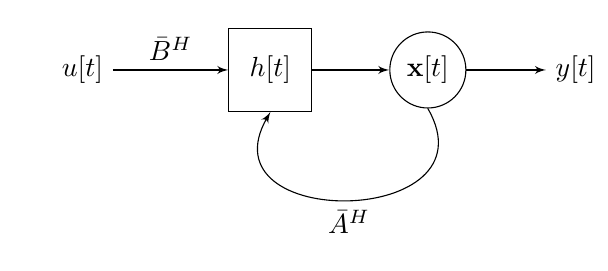
\begin{tikzpicture}[auto, >=latex']
    \node [input, label=left:{$u[t]$}] (u) {};
    \node [block, right of=u, node distance=2cm] (h) {$h[t]$};
    \node [ensemble, right of=h, node distance=2cm] (x) {$\V{x}[t]$};
    \node [output, label=right:{$y[t]$}, right of=x, node distance=1.5cm] (y) {};
    \draw [->] (u) -- node {$\bar{B}^H$} (h);
    \draw [->] (h) -- (x);
    %\draw [->] (x.north) -- (y);
    \draw [->] (x) -- (y);
    %\draw [->] (x.south) -- (y);
    \path[->] (x.south) edge [loop below, min distance=5em, out=-60, in=-120] node {$\bar{A}^H$} (h.south);
  \end{tikzpicture}
  \caption[Model of the Delay Network for digital architectures.]{ \label{fig:delay-architecture}
    Delay Network~(DN) model for a digital architecture.
    The synapse $h[t]$ is driven by $\bar{A}^H \V{x}[t] + \bar{B}^H u[t]$ to yield the state $\V{x}[t]$.
    This state is nonlinearly encoded by a heterogeneous population of neurons and subsequently decoded to estimate the desired $y[t]$.
  } 
\end{figure}

In all cases, we construct a reservoir of $\numprint{1500}$ neurons, and then train separate linear readouts to approximate various delays ranging from $100$--$200$\,ms ($\dt{} = 1$\,ms).
For the NEF case, the prescribed dynamical system is a $\theta = 200$\,ms delay, implemented by mapping equation~\ref{eq:ss-delay} onto a discretized lowpass (see equation~\ref{eq:discrete-p3}).
In section~\ref{sec:delay-lstm} we show that the delay length can be trained from raw data.
Importantly, the same networks are used to compute all of the different delays reported.
We thus conceptualize the DN as an optimized ``low-dimensional reservoir''.
%The input to each network is randomly sampled $25$\,Hz band-limited white noise.
Compiling all of the equations of this network, for clarity (see Figure~\ref{fig:delay-architecture}):
\begin{equation} \label{eq:delay-compiled}
\begin{aligned}
v_i &= \frac{(q+i)(q-i)}{i+1} \theta^{-1} \text{,} \quad i = 0 \ldots q-1 \\
A &= \begin{pmatrix} -v_0 & -v_0 & \cdots & -v_0 \\ v_1 & 0 & \cdots & 0 \\ 0 & \ddots & \ddots & \vdots \\ 0 & 0 & v_{q-1} & 0\end{pmatrix} \in \mathbb{R}^{q \times q} \\
B &= \transpose{\begin{pmatrix} v_0 & 0 & \cdots & 0\end{pmatrix}} \in \mathbb{R}^{q} \\
\bar{A} &= \sum_{i=0}^\infty c_i A^i = \sum_{i=0}^\infty \frac{\left(A\dt{}\right)^i}{i!} = e^{A\dt{}}  \\
\bar{B} &= \left( \sum_{i=1}^\infty c_i A^{i-1} \right) B = A^{-1} \left(\bar{A} - I\right) B  \\
a &= e^{-\frac{\dt{}}{\tau}} \\
\bar{A}^H &= \frac{1}{1 - a} \left(\bar{A} - aI\right) \\
\bar{B}^H &= \frac{1}{1-a}\bar{B} \text{.}
\end{aligned}
\end{equation}
We remind the reader that $A$ and $B$ may be transformed by any of the state-space realizations from section~\ref{sec:software} before proceeding with the remaining numerical machinery.
The final matrices $(\bar{A}^H\text{,}\, \bar{B}^H)$ determine the transformations to be implemented using Principles~1 and~2 of the NEF, which in turn will nonlinearly encode $\V{x}[t]$ by our extensions to Principle~3.

\begin{figure}
  \centering
  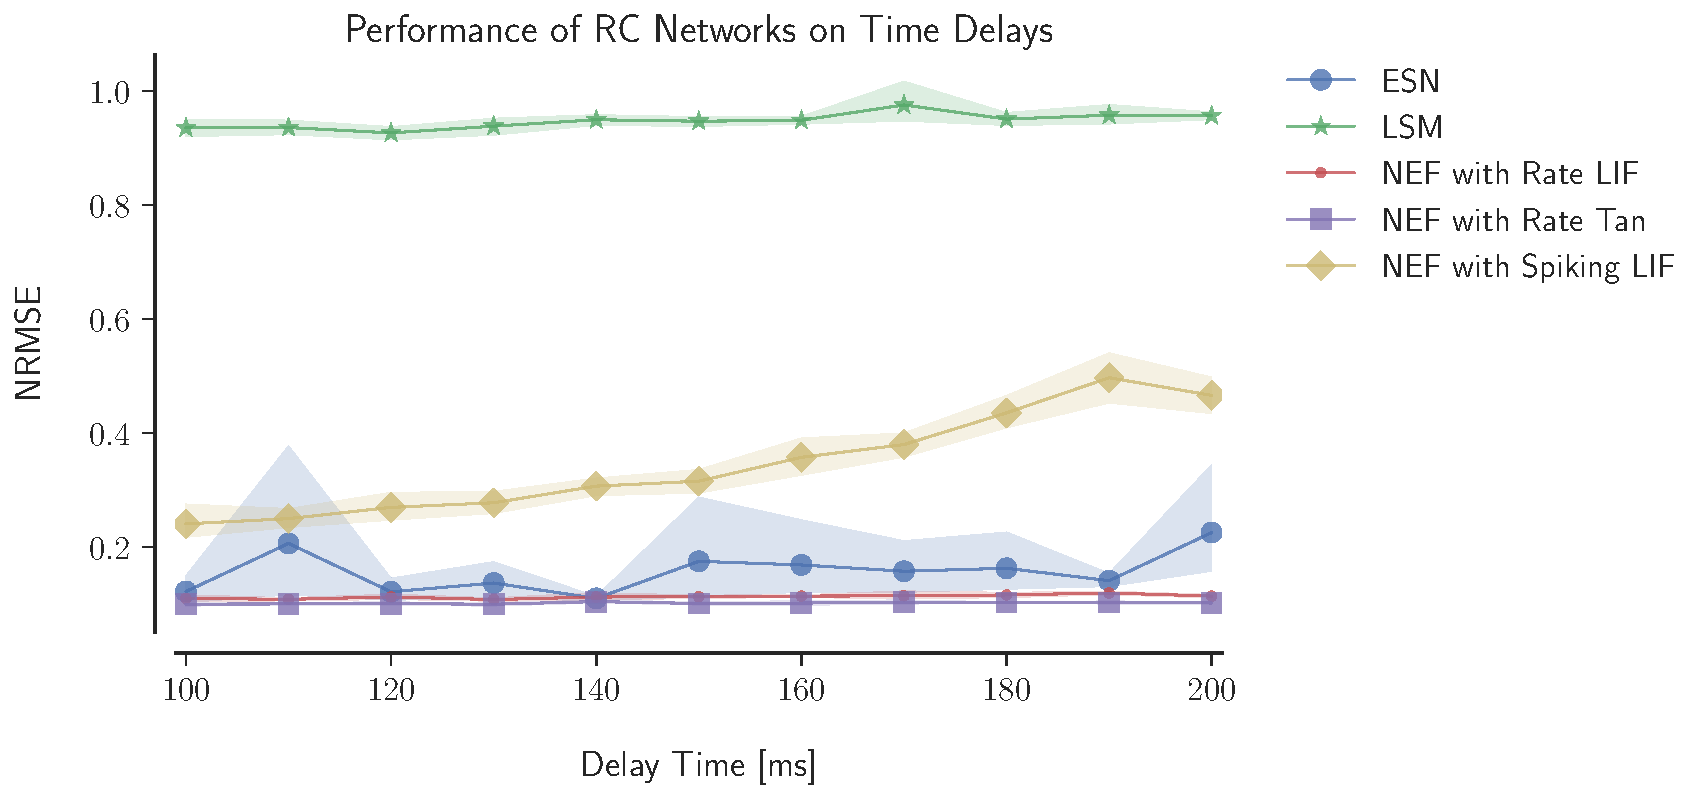
\includegraphics[width=0.8\textwidth]{rc-accuracy}
  \caption[Accuracy of Reservoir Computing versus the NEF.]{ \label{fig:rc-accuracy}
  Performance from training various linear readouts to compute delays of $25$\,Hz band-limited white noise (bootstrapped across 10 trials).
  Each line corresponds to a single reservoir of $\numprint{1500}$ neurons, either randomly connected (in the case of ESNs and LSMs), or specifically engineered (in the case of the NEF).
  }

  \vspace{1em}

  \centering
  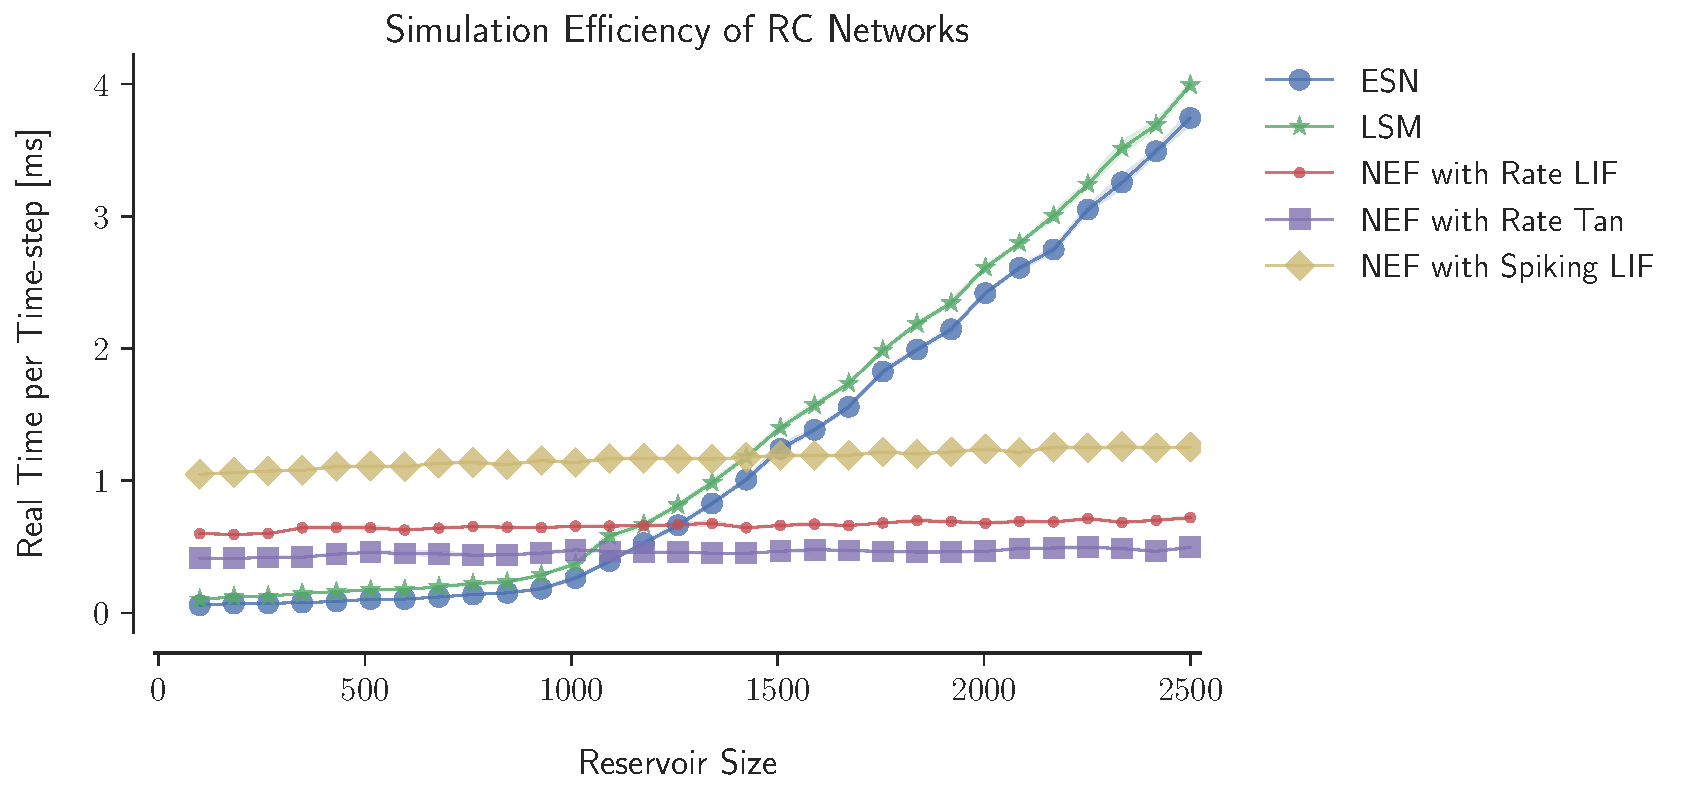
\includegraphics[width=0.8\textwidth]{rc-speed}
  \caption[Efficiency of Reservoir Computing versus the NEF.]{ \label{fig:rc-speed}
  Cost of simulating each RC network as the reservoir size is increased (bootstrapped across 10 trials).
  Conventional RC approaches require $\bigoh{ n^2 }$ space and time, while the NEF improves this to $\bigoh{ n }$ for constant dimensionality.
  }
\end{figure}

As shown in Figure~\ref{fig:rc-accuracy}, the NEF's performance is slightly better than ESNs for both LIF rate neurons and $\tanh$ rate neurons, and significantly better than LSMs for spiking LIF neurons.
This demonstrates that, in terms of memory capacity, the DN as a low-dimensional reservoir not only outperforms RC in the rate-based case, but even performs comparably to ESNs when using spikes.
The task is shown to be completely outside the grasp of LSMs (exceeding $90$\% error), due to the difficulty of the computation and the unreliability of randomized spiking feedback; HyperOpt minimizes both the gain and regularization hyperparameters of the LSM to keep its output close to zero, as this minimizes validation error.\footnote{%
As additional validation, lower input frequencies or shorter delay lengths were possible with the LSM.}
The success of the DN should not be surprising given that we have mapped the ideal delay's dynamics onto the reservoir.
Nevertheless, as we will show below, the readouts are capable of computing nonlinear functions across the delay interval, from the same reservoir.
%This demonstrates that our derived state-vector (see Figure~\ref{fig:pca}) is robust to changes in the target function.
Informally, assigning some particular dynamics to the reservoir does not disable the network from computing other similar functions (thereby permitting nonlinear combinations of such functions to be trained from data).

These networks were also simulated while varying the number of neurons from $100$ to $\numprint{2500}$, in order to measure the real-time cost of simulation (see~Figure~\ref{fig:rc-speed}).
We again note that traditional RC suffers from scaling issues since the recurrent weight matrices have $\bigoh{ n^2 }$ coefficients.
Consequently, the NEF is more resource efficient than these RC methods by a factor of $\bigoh{ n }$.
RC networks often include a sparsity constraint of $20\%$ connectivity, which is still $\bigoh{n^2}$, in order to improve performance~\citep{lukovsevivcius2012practical, lukovsevicius2012reservoir}.
We also considered ESNs with constant sparsity that balance resource constraints with NEF networks, but found that they did not perform comparably (not shown).
Furthermore, we found that the ESN breaks down for numbers of neurons as few as $q$ neurons, while in fact $q$ linear rate neurons (with linearly independent encoders) will suffice to perfectly implement equation~\ref{eq:ss-delay}, as $q$ linear state-variables are in exact correspondence with the ideal linear system (after the appropriate discretization of equation~\ref{eq:discrete-p3}) (see section~\ref{sec:force-comparison}).

\begin{table}\centering
  %\ra{1.2}
  \noindent\begin{tabularx}{\textwidth}{YYYYYY}
    \toprule
     & ESN & LSM & NEF with Rate LIF & NEF with Rate Tan & NEF with Spiking LIF \\
    \midrule
Gain & \num[round-precision=3,round-mode=figures,scientific-notation=true]{1.3251896701} & \num[round-precision=3,round-mode=figures,scientific-notation=true]{0.00315170551016} & - & - & - \\

Radius & \num[round-precision=3,round-mode=figures,scientific-notation=true]{24.3145093319} & \num[round-precision=3,round-mode=figures,scientific-notation=true]{1.36259213791} & \num[round-precision=3,round-mode=figures,scientific-notation=true]{4.63655157006} & \num[round-precision=3,round-mode=figures,scientific-notation=true]{12.8794579757} & \num[round-precision=3,round-mode=figures,scientific-notation=true]{0.577484080063} \\

$\tau_\mathrm{readout}$ & \num[round-precision=3,round-mode=figures,scientific-notation=true]{0.00686793487811} & \num[round-precision=3,round-mode=figures,scientific-notation=true]{0.0604400629751} & \num[round-precision=3,round-mode=figures,scientific-notation=true]{0.0606008691858} & \num[round-precision=3,round-mode=figures,scientific-notation=true]{0.0873173665926} & \num[round-precision=3,round-mode=figures,scientific-notation=true]{0.0218081523547} \\

$\tau_\mathrm{recurrent}$ & \num[round-precision=3,round-mode=figures,scientific-notation=true]{0.0021441109352} & \num[round-precision=3,round-mode=figures,scientific-notation=true]{0.069089989522} & \num[round-precision=3,round-mode=figures,scientific-notation=true]{0.0626041764586} & \num[round-precision=3,round-mode=figures,scientific-notation=true]{0.0937145408042} & \num[round-precision=3,round-mode=figures,scientific-notation=true]{0.0740410932649} \\

$\sigma^2_\mathrm{readout}$ & \num[round-precision=3,round-mode=figures,scientific-notation=true]{2.95578336256e-06} & \num[round-precision=3,round-mode=figures,scientific-notation=true]{0.0329425610169} & \num[round-precision=3,round-mode=figures,scientific-notation=true]{0.00206289719197} & \num[round-precision=3,round-mode=figures,scientific-notation=true]{0.00479755699712} & \num[round-precision=3,round-mode=figures,scientific-notation=true]{0.0450158827701} \\

$\sigma^2_\mathrm{recurrent}$ & - & - & \num[round-precision=3,round-mode=figures,scientific-notation=true]{0.000200121787175} & \num[round-precision=3,round-mode=figures,scientific-notation=true]{0.000397747221121} & \num[round-precision=3,round-mode=figures,scientific-notation=true]{0.0375517001869} \\

$q$ & - & - & 20 & 26 & 23 \\

    \bottomrule
  \end{tabularx}
  
  \caption{ \label{tab:hyperopt}
    HyperOpt parameters for the linear benchmark in section~\ref{sec:delay-rc}.
  }
\end{table}

Another key finding is that, as shown in Table~\ref{tab:hyperopt}, 
HyperOpt discovers that a radius of $\approx 24.3$ performs the best with the ESN.
This has the effect of scaling the domain of the tanh curve from $[-1, 1]$ to $\approx [-0.04, 0.04]$, which importantly is well-approximated by a straight line, that is, $\tanh x \approx x$ across this domain.
Thus, HyperOpt is indirectly leveraging the fact that the ESN's memory capacity is maximized when its neurons \emph{are linear}, consistent with \citet{dambre2012information}.
Crucially, this limits the ability of the ESN to perform nonlinear computations across the delay interval, as we now show.

\subsubsection{Nonlinear benchmark}

To demonstrate our ability to compute nonlinear window functions, we consider the function from section~\ref{sec:delay-nonlinear}, $y(t) = u(t - \theta)\, u(t)$, visualized in the context of a DN's state-vector in Figure~\ref{fig:delay-autocorrelation}.
When integrated over time, this is the autocorrelation of $u$ with lag $\theta$, which has numerous applications in signal processing (e.g.,~detecting repeating events).
We fix $\theta = 0.1$\,s across all experiments.
To compute this function accurately, we sample a proportion of the encoders from the diagonal combinations of $\mathcal{P}_{i, d}(0)$ and $\mathcal{P}_{i, d}(1)$~\citep{jgosmann2015}.
However, the particular choice of function is not of importance, as the training can be data-driven, or analyzed using theory from sections~\ref{sec:temporal-representation} and~\ref{sec:delay-nonlinear}.

Each input $u(t)$ is sampled white noise, band-limited with a cutoff frequency of $30$\,Hz.
To optimize for the decoders, we map $q$-dimensional evaluation points onto desired target outputs using equation~\ref{eq:basis-interpretation}, and apply Nengo's regularized least-squares solver, which bypasses the need to explicitly simulate the network on any input signals.

To implement this system as a spiking (or non-spiking) recurrent neural network, we use the same set of transformations from equation~\ref{eq:delay-compiled}. % Principle~3 of the NEF to map equation~\ref{eq:delay-system} onto the dynamics of the synapse.
%For example, repeating the standard form of Principle~3 for a continuous-time lowpass synapse with time-constant $\tau$ (although we are free to use the extensions of chapter~\ref{chapt:nef-extensions}):
%\begin{equation} \label{eq:delay-system-p3}
%A^H = \tau A + I \text{,} \quad B^H = \tau B \text{,} \quad H(s) = \left(\tau s + 1\right)^{-1} \text{.}
%\end{equation}
The model architecture of this delay network is, again, depicted in Figure~\ref{fig:delay-architecture}, whose representation and transformations are realized using the NEF.
For this experiment, we considered the use of both sigmoidal (non-spiking) neurons, and spiking LIF neurons.

We again used HyperOpt~\citep{bergstra2015hyperopt} to explore the space of model hyperparameters (e.g.,~$q$, $\tau$, input gain, recurrent gain, L2-regularization) across $100$ iterations containing $10$ trials each.
Each network consisted of $\numprint{1000}$ neurons, simulated with a time-step of $\dt{} = 1$\,ms.
Each trial used a training signal of length $\numprint{10200}$, a testing signal of length $\numprint{2200}$, and the first $200$ outputs were discarded.
We then cross-validated the best set of hyperparameters (in terms of mean NRMSE across all test signals) using another $25$ trials.

We obtain a mean NRMSE of $5.9$\% for the sigmoid DN, $51.8$\% for the spiking DN, and $84.3$\% for the $\tanh$ ESN.
Reducing the input frequency from $30$\,Hz to $15$\,Hz improves the ESN's accuracy to be on par with the non-spiking DN, and thus we attribute this difference to the inherent difficulty of autocorrelating a high-frequency signal (relative to $\theta$) using random feedback weights, as opposed to using optimally derived weights as in the DN.
In addition, trials took on average $5.10$\,s for the sigmoid DN, $6.44$\,s for the spiking DN, and $17.7$\,s for the ESN.
This difference is a consequence of not simulating the DN for training, and from using factorized weight matrices (i.e.,~encoders and decoders) to simulate the DN.
These results are consistent with that of the linear benchmark, except for the additional observation that here the spiking DN outperforms the rate ESN.
This is because, as explained previously, the ESN's memory capacity requires linear tuning, which is at odds with the nonlinearities required by functions such as autocorrelation.
LSMs were again unable to perform the task.

\TODO{We should be able to dramatically improve this spiking result...}

\subsection{Force learning}
\label{sec:force-comparison}

We also compared our NEF solution to both FORCE~\citep{sussillo2009generating} and full-FORCE~\citep{depasquale2018full} networks (also see sections~\ref{sec:engineered-approaches} and~\ref{sec:relationships}).
FORCE networks take the same essential ingredient of RC networks, namely the inclusion of high-dimensional random feedback, except they make an important addition to the model: the target output is learned---online via RLS---to be simultaneously re-encoded back into the network (see Figure~\ref{fig:architectures}).
Full-FORCE takes this a step further, by using the (pre-filtered) currents from from the previous FORCE network as a training signal for a separate ``full-FORCE'' network. 
In the first step, the FORCE network does not do any online learning, but instead receives the exact ideal teaching signal.
The second step then allows for additional degrees of freedom to be optimized, to find the \emph{full weights} that reconstruct the ideal currents from the first network -- again, online using RLS.
This is similar in many ways to \citet{tripp2006neural}, but maintains the same idea as in FORCE, in particular the re-encoding of the target state.
The main difference from FORCE is that instead of learning a low-rank (one-dimensional) decode-encode of the target, full-FORCE learns a full-rank approximation to an encoding of that same target.

For this experiment, we first ported the same implementation described in \citet{depasquale2018full} to Nengo, and verified that it is works as intended (using the same models and parameters) by teaching the network to produce decaying oscillations in response to unit impulses.
We compared this to the standard FORCE approach---which we refer to as ``classic-FORCE''---and verified that it performed slightly worse than the full-FORCE network, but still better than an equivalent reservoir computer.
Since Nengo allows for the substitution of various spiking and non-spiking neuron models, we further validated both implementations with spiking neurons as well, and obtained reasonable levels of accuracy, similar to \citet{depasquale2016using, thalmeier2016learning, nicola2016supervised}.

However, we found that simply modifying the target signal to be a delayed version of its low-frequency input signal, posed a significant challenge to these networks.
Thus, the learning rate was lowered from $1$ to $\numprint{e-3}$, and the time-step set to $\dt{} = 5$\,ms, which we found to help regularize the solution.
We thus also considered a baseline approach:
we took the original FORCE network, but removed the feedback loop that re-encodes the learned output.
This makes it equivalent to an ESN with a slightly different method of distributing the weights, while learning the decoders online.
We refer to this last method as ``no-FORCE''.

We now compare all three of these to an idealized NEF implementation of the DN~(equation~\ref{eq:ss-delay}), consisting of just $n = 6$ linear units, coupled to one another by the discretized mapping of equation~\ref{eq:discrete-p3}, as summarized by equation~\ref{eq:delay-compiled} ($q = 6$).
In this scenario, the only error that remains is that of equation~\ref{eq:pade-delay-error} arising from the use of Pad\'e approximants to render the delay line finite-dimensional.
Each FORCE network consists of $n = 500$ neurons (and $\bigoh{n^2}$ weights).
The network is given $10$\,s of training data per trial.
In all cases, the training and test signals are randomly sampled $1$\,Hz band-limited white noise signals, with $5$\,s of test data per trial.
We compare all four networks by sweeping $\theta$ across $0.01$--$1$\,s, with $10$ trials at each value of $\theta$ (bootstrapped 95\% confidence intervals).

\fig{force-comparison}{0.7}{Memory capacity of FORCE versus the NEF.}{
    Comparison of several FORCE learning methods versus the NEF on a delay task.
    Networks are trained to delay a time-varying input by $\theta$ seconds.
    Each FORCE network consists of $500$ $\tanh$ neurons, while the NEF network is $6$ linear neurons.
    See text for details.
}

The results in Figure~\ref{fig:force-comparison} illustrate that the NEF's six rate neurons outperform all of the FORCE networks.
The full-FORCE network performs well relative to classic-FORCE and no-FORCE for short delays ($\theta < 0.1$\,ms).
For longer delays ($\theta > 0.1$\,s), the classic-FORCE network performs well relative to the other two, but still with error-rates approaching $100$\% as $\theta \rightarrow 1$\,s, or $200$ time-steps.
This reveals a situation in which training the network to re-encode its target output can hinder performance.
The NEF solution proposes a means of understanding this phenomenon.
In particular, the target output is only one dimension among six orthogonal dimensions that must all be encoded into the state of the network.
Focusing on this one dimension and letting the randomized feedback attempt to fill in the rest, leads to competing objectives between the low-dimensional linear feedback required for optimal memory capacity and the high-dimensional chaos induced by nonlinear random feedback.

\subsection{Long short-term memory}
\label{sec:delay-lstm}

Long Short-Term Memory~\citep[LSTM;][]{hochreiter1997long, gers1999learning} networks address the problem of storing information across long intervals of time by using an explicit memory unit to alleviate the vanishing and exploding gradient problems~\citep{bengio1994learning, bengio1994credit}.
Each memory unit implements a small-scale dynamical system---similar \emph{in spirit} to equation~\ref{eq:delay-compiled}---referred to as an ``LSTM cell'', with a number of free parameters that control its nonlinear transfer function.
This is replicated $n$ times to create a single layer.
Each layer is then stacked $k$ times to form a ``stacked LSTM'', with each consecutive layer representing increasingly higher-order dynamical transformations of its previous inputs~\citep{graves2013speech}.

Since all of these mechanisms are differentiable, backpropagation through time~(BPTT) may be applied end-to-end from raw data to optimize all of the parameters in a black-box manner (see section~\ref{sec:bptt}).
Recently, this has found numerous successes in sequence learning, machine translation, and speech~\citep{graves2013speech, sutskever2014sequence, cho2014learning, bahdanau2014neural}, leading to a widespread adoption of LSTM networks as the RNN of choice~\citep{lecun2015deep}.

However, we find that when given a continuous-time delay task, the performance of stacked LSTMs suffer catastrophically in the number of time-steps that roll through the memory.
This motivates the substitution of each ``LSTM cell'' with our Delay Network~(DN)---explored extensively throughout this chapter---and its subsequent training via backpropagation in an equivalent manner.
We now discuss these experimental results.

\subsubsection{Memory capacity}

Our first set of experiments are designed to evaluate the memory capacity of stacked LSTMs relative to stacked Delay Networks of equivalent resource usage.
For this, we use an off-the-shelf implementation of a stacked LSTM~\citep[Keras;][]{gulli2017deep}, and construct $k=3$ layers with $n=50$ cells each.
Each layer is fully-connected to the next, and uses all of the default settings (e.g.,~$\tanh$ activations).
The final layer likewise consists of a $\tanh$ activation unit for each output.

To evaluate the continuous-time memory capacity, the input data is white noise, band-limited to $30$\,Hz, starting at $0$, and normalized to an absolute range of $[-1, 1]$.
The output data is a $50$-dimensional vector representing a uniform arrangement of delayed inputs between $0$--$0.2$\,s.\footnote{%
Therefore, the highest frequency component oscillates at most six times, within any given delay interval.
}
The data set consists of $256$ samples, each $1$\,s long.
This data is randomly partitioned into $50$\% training and $50$\% testing.
The training data is further partitioned into a separate random $25$\% sample used to report validation accuracy during training.
Backpropagation through time is carried out using the Adam optimizer~\citep{kingma2014adam} with respect to the MSE loss function.
Training is parallelized using Keras and TensorFlow~\citep{abadi2016tensorflow} across four Nvidia Titan Xp GPUs (12\,GB each).\footnote{%
This took approximately 14 hours in our largest experiment, in stark contrast to the sub-second time that it takes to train a spiking delay network using Nengo.}

\TODO{Show shorter delay experiment.}

We found that, for a time-step of $\dt{} = 2$\,ms, backpropagation could find adequate parameters to solve this task -- that is, the LSTM could in fact accurately represent the entire delay interval consisting of $\bar{\theta} = 100$ time-steps with an NRMSE of about 10\% (not shown).
However, after decreasing the time-step, by an order of magnitude, to $\dt{} = 200$\,$\mu$s---while increasing the length of data by the same factor so that the data still represents the exact same $1$\,s signals---the performance collapses; accuracy exponentially decays as a function of delay length across the $\bar{\theta} = \numprint{1000}$ time-step window (see Figure~\ref{fig:lstm-capacity}~(b)).

\TODO{Run again with linear units on the output layer. Move the tanh in the DN cell to the input rather than output.}

We then took the exact same code and network specification -- but replaced each LSTM cell with a ``Delay Network~(DN) cell'', defined as follows.
We consider the $q$-dimensional LTI system described by equation~\ref{eq:delay-system}, with a balanced state-space (section~\ref{sec:software}), and discretized using Euler's method:
$$\V{x}[t+1] =  \bar{\theta}^{-1} \left( A \V{x}[t] + B u [t] \right)] + \V{x}[t] \text{.}$$
This discretization assumes $\bar{\theta}$ is sufficiently large, such that $\dt{} \approx \bar{\theta}^{-1}$.
This ``trick'' enables us to include $\bar{\theta}$ as a free parameter, unique to each cell, and backpropagate along it -- thus learning the delay length of each cell.
The unit of this discretized $\bar{\theta}$ is the number of time-steps.
This is repeated across all cells within the same layer, while \emph{sharing} the $(A, B)$ matrices across each cell within the same layer (akin to weight-sharing in a convolutional neural network).
Finally a $\tanh$ nonlinearity is added to each unit, that receives input from all state-variables across the same layer, thus supporting nonlinear computations across a mixture of scaled Legendre bases (see section~\ref{sec:delay-nonlinear}).
For small values of $q$, the DN cell is roughly comparable to the resource requirements of the original stacked LSTM model, using $q$ state-variables, $\bigoh{q^2}$ multiply-adds, and $1$ nonlinearity with $qn$ weights, per cell.

Each DN cell receives a one-dimensional input. The trainable parameters are the weights between layers, and the delay lengths $\bar{\theta}$ within each cell.
In this experiment, we disable training on the shared $(A, B)$ weights.
The overall architecture remains fixed with $n$ cells stacked $k$ times.
The final output layer consists of linear activation units, since $\tanh$ has already been applied at this point.
Finally, we fix $q=9$, initialize the encoding weights of each cell to $1$ for the first layer and $n^{-1}$ for all subsequent layers~(i.e., the reciprocal of the fan-in), distribute $\bar{\theta}$ values according to $\mathcal{U}[100, 1000]$, and set the weights projecting to each $\tanh$ using the $C$ matrix from equation~\ref{eq:delay-system} with zero weights for all other state-variables from outside the cell.
In other words, each cell is \emph{initialized} to approximate $\tanh u[t - \bar{\theta}]$, where $u[\cdot]$ is the cell's mean input.
Backpropagation then refines the values of $\bar{\theta}$ and learns to mix weighted nonlinear combinations of inputs and outputs between layers.

\begin{figure}
  \centering
  \begin{subfigure}{.5\textwidth}
    \centering
    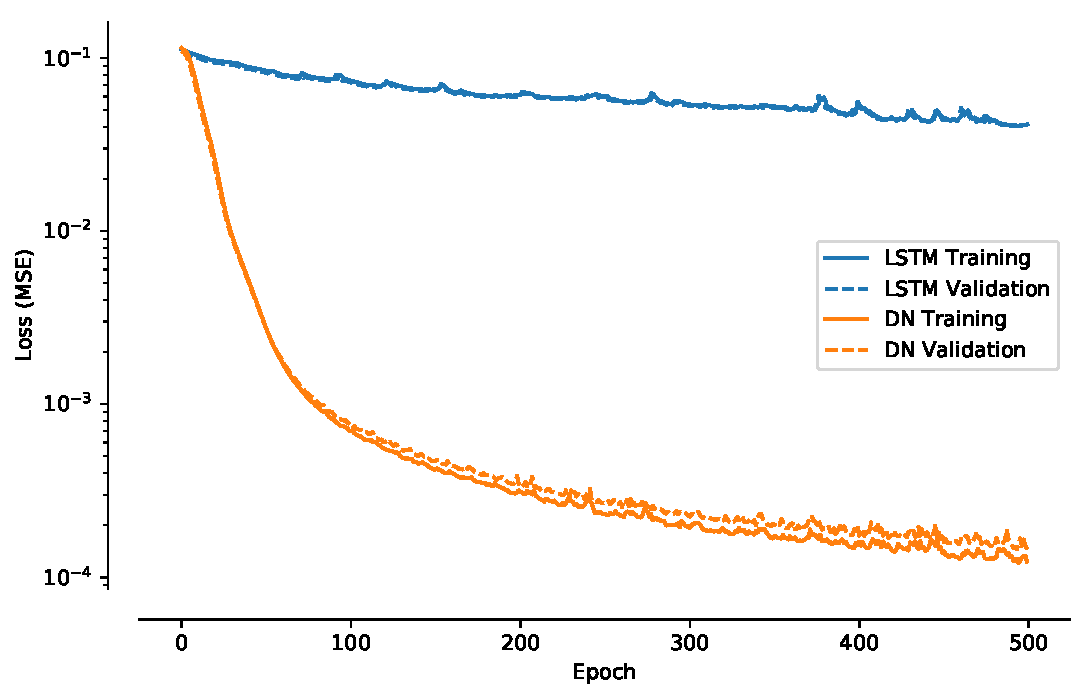
\includegraphics[width=\linewidth]{lstm-capacity-training}
    \caption{Training \& Validation}
  \end{subfigure}%
  \begin{subfigure}{.5\textwidth}
    \centering
    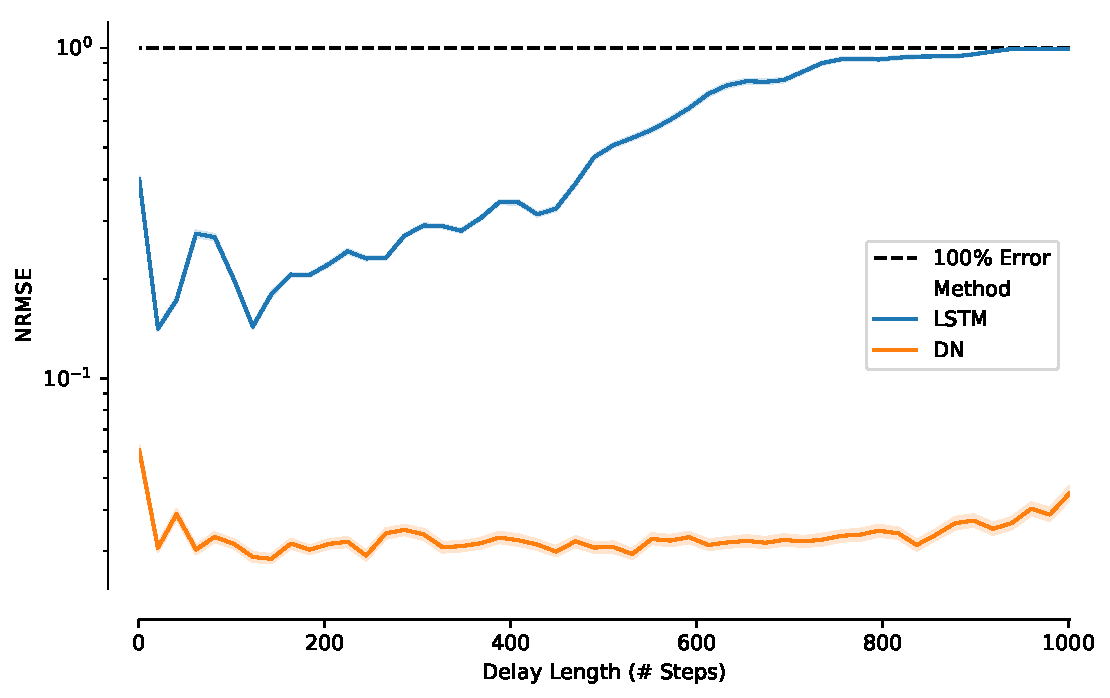
\includegraphics[width=\linewidth]{lstm-capacity-testing}
    \caption{Testing}
  \end{subfigure}
  \caption[Memory capacity of a stacked LSTM versus Delay Network.]{\label{fig:lstm-capacity}
    Performance of a stacked LSTM versus a stacked Delay Network~(DN) on a delay task.
    (a)~Training and validation rapidly converge for the DN but not for the LSTM.
    (b)~Testing NRMSE is nearly uniform across the delay interval for the DN, 
    but grows exponentially for LSTMs (linear on a log-scale) up to a maximum of $100$\% error.
    See text for details.
  }
\end{figure}

\TODO{Show experiment with longer time-step.}
\TODO{Fit line to (b)-LSTM.}

Running the exact same code and analysis, on the exact same training, validation, and testing data, reveals a dramatic difference in training time between the two approaches.
We found that the stacked DN takes $52.5$\,s per epoch to train, compared to $102.6$\,s per epoch for the stacked LSTM.
Furthermore, the DN outperforms the LSTM in every measure of accuracy.
Figure~\ref{fig:lstm-capacity}~(a) demonstrates nearly three orders of magnitude reduction in MSE across both training and validation, while converging much more rapidly to the ideal solution.
Figure~\ref{fig:lstm-capacity}~(b) displays the NRMSE on the test data as a function of delay length (unit of time-steps).
We see that the DN architecture achieves nearly uniform accuracy across the delay interval, while the equivalently-sized LSTM cell architecture approaches $100$\% error rates towards the end of the window.
This illustrates that the stacked LSTM struggles to memorize low-frequency signals (relative to the time-step) across long intervals of time.
In contrast, this task is natural for the stacked DN, as its state represents a $q$-degree polynomial expansion of input history (see Figure~\ref{fig:basis-functions}).
We now proceed to demonstrate that backpropagation enables the stacked DN cells to outperform the stacked LSTMs even on tasks that are not readily supported by the initial configuration of the network.

\subsubsection{Predicting chaotic time-series}

\fig{mackey-glass-example}{1}{Example test case from the Mackey-Glass dataset.}{
    Example test case from the Mackey-Glass~(MG) dataset ($\bar{\tau} = 17$).
    $x$ is the input. $y$ is the correct prediction $15$ time-steps into the future. We plot $x$ versus the difference between the required prediction and the input, $y - x$, which also shows a two-dimensional delay-embedding of the attractor. 
    The signal consists of $\numprint{5000}$ time-steps ($0$ is lightest, $\numprint{4999}$ is darkest), with a line connecting adjacent time-points.
}

\noindent 
To asses the performance of each network on a continuous-time prediction task, we consider a synthetic dataset called Mackey-Glass~\citep[MG;][]{mackey1977oscillation}: a chaotic time-series described by a nonlinear delay-differential equation.\footnote{%
Our code was adapted from the 2015 Deep Learning Summer School: \url{https://github.com/mila-iqia/summerschool2015/blob/master/rnn\_tutorial/synthetic.py}.
}
The MG data is generated using a discrete time-delay of $\bar{\tau} = 17$ (each time-step is $1$ unit of time).
The desired output is a look-ahead (prediction) of $15$ time-steps in advance (see Figure~\ref{fig:mackey-glass-example}).
We simulate this for $\numprint{5000}$ time-steps after removing the first $100$ step transient.
We repeat this $128$ times, each time starting from initial random conditions.
The entire dataset is then centered to have a global mean of zero.
Next, the dataset is randomly split into $32$ training examples, $32$ validation examples, and $64$ testing examples.

We use the same networks from the previous experiment, but with $k = 4$ layers of $n = 100$ cells each.
For the DN cells, we make all parameters trainable (including the $A$, $B$ matrices shared across cells within the same layer).
We set $q=6$ and initialize $\bar{\theta} \in \mathcal{U}[25, 50]$ to account for the shorter time-scale of this dataset.
We initialize the remaining weights using standard Keras weight initializers.

To successfully solve this problem, the RNN must implicitly do two things.
First, it must model the dynamics of the state-trajectory to infer the underlying state from a one-dimensional observation.
A theorem due to \citet{takens1981detecting} states that this is made possible by delaying the input some constant number of times (dependent on $\bar{\tau}$) and then finding the correct static nonlinear transformation of this ``delay embedding.''
Second, it must predict the future state of this trajectory using its estimate of the current state.
The last step is generally infeasible due to the chaotic nature of the MG system; \emph{any} finite error in the state estimate is exponentially magnified over time (the ``butterfly effect''; also see section~\ref{sec:chaos}).
This makes a look-ahead of $15$ steps particularly challenging for a relatively small network, as its reconstruction of the chaotic manifold must become exponentially more precise to see linear payoffs in accuracy.

This insight motivates the inclusion of a third ``hybrid'' method that interleaves the two previous methods. Specifically as in `\texttt{2121}', where `\texttt{2}' is the DN cell and `\texttt{1}' is the LSTM cell.
The total resource requirements are still roughly the same.
All three methods are trained across $500$ epochs using the Adam optimizer.
In this case, to minimize overfitting, we keep only the model from the epoch that has the highest validation score. 

Test performance and training times are summarized in Table~\ref{tab:mackey-glass}.
We see that the DN outperforms the LSTM in accuracy and training time.
We suspect that this is because the DN more readily supports a delay-embedding within its $6$-dimensional state.
However, the hybrid method outperforms both in accuracy and the LSTM in training time.
Thus, the LSTM cell affords some dynamical primitive that may be leveraged by networks of DN cells (and vice-versa).
This suggests that LSTMs and DNs may have complementary functions as building blocks within deep RNNs.
And, as shown in our first experiment, the DN provides improved scaling through time with respect to lower frequencies across longer continuous time-intervals.

\begin{table}
\centering
  \begin{tabular}{@{}lrr@{}} \toprule
    Method & NRMSE & \pbox{20cm}{Training Time \\ ($s$ / epoch)} \\
    \midrule
LSTM & 7.084\% & 50.0 \\
DN & 6.783\% & 30.5 \\
Hybrid & 6.097\% & 40.5 \\
    \bottomrule
  \end{tabular}
  \caption[Prediction accuracy of a stacked LSTM versus Delay Network.]{ \label{tab:mackey-glass}
    Test accuracy and training time for various RNNs on the Mackey-Glass~(MG) dataset.
  }
\end{table}

\subsection{Detecting patterns}
\label{sec:periodicity}

We now demonstrate an application of our theory of temporal representation in the delay network (section~\ref{sec:temporal-representation}).
Specifically, we show that the delay network can detect the existence of repeating patterns in its stimulus.
Given an arbitrary scalar signal, $u(t)$, we define a measure of \emph{$k$-periodicity} for natural $k \in \mathbb{N}_{\ge 1}$, with respect to some finite interval length $\theta > 0$, and sub-interval length $\gamma = \theta k^{-1}$, as follows:
\begin{equation} \label{eq:periodicity}
p_k(t) = \sqrt{ \frac{1}{\gamma} \int_{\tau=0}^{\gamma} \left( \frac{1}{k} \sum_{i=0}^{k-1} u \left( t - \theta + i \gamma + \tau \right) \right)^2 d\tau } \text{.}
\end{equation}
This can be computed directly by: (1) partitioning the last $\theta$ seconds into $k$ equally sized segments of length $\gamma$, (2) averaging them all together to obtain a superimposed signal of length $\gamma$, and (3) taking its root mean square (RMS).
When $p_k(t)$ is large relative to the overall RMS, this means that the $k$ segments constructively interfere and thus all segments contain approximately the same pattern. 
When $p_k(t)$ is maximal (i.e.,~equal to the RMS of the input signal), we refer to the signal  as being \emph{periodic}, since each of the $k$ segments must be exact copies of one another.
Lower values of $p_k(t)$ imply some amount of deconstructive interference within the superposition, and thus we refer to such signals as being \emph{aperiodic}.

We now present a method that can efficiently compute $p_k(t)$ with a SNN, by leveraging the computational properties of the DN.
This has applications as a general low-power signal processing tool, and for modelling how nontrivially-repeating patterns could be detected by neural mechanisms in a robust and flexible manner.

Our goal is to recast equation~\ref{eq:periodicity} to be in terms of the DN's state-vector, $\V{x}(t) \in \mathbb{R}^q$.
We claim that we may compute $p_k(t)$ by taking the L2-norm of the state-vector after a linear transformation:
\begin{align} \label{eq:approx-periodicity}
p_k(t) &\appropto \| P_k \V{x}(t) \| \\
P_k &= \frac{Z_k}{k} \sum_{i=0}^{k-1} e^{A i \gamma} \text{,} \label{eq:periodicity-matrix}
\end{align}
where $A$ is the recurrent state-space matrix from the balanced realization of equation~\ref{eq:ss-delay},\footnote{%
The proportionality $\propto$ in equation~\ref{eq:approx-periodicity} refers to a constant scaling in the balanced realization, while the approximation $\sim$ comes from the use of Pad\'e approximants to render the system finite-dimensional, and from assuming the DN mapping is unitary.
See text for details.
}
and $Z_k \in \mathbb{R}^{q \times q}$ is a ``zooming matrix'' computed by:
\begin{equation} \label{eq:zoom-matrix}
Z_k = B(0, 1)^+ B(1-1/k, 1) \text{,} % = \left( \transpose{B(0, 1)} B(0, 1) \right)^{-1} \transpose{B(0, 1)} B(1-1/k, 1) \text{,}
\end{equation}
where $(\cdot)^+$ denotes the Moore-Penrose pseudo-inverse, $B(\cdot, \cdot) \in \mathbb{R}^{m \times q}$ is a matrix corresponding to a slice of the realized basis functions (equation~\ref{eq:basis-functions}), sampled along $m$ points, as in:
\begin{equation}
B(a, b) = \begin{pmatrix}
\mathcal{P}_{q-1,q}(a) & \cdots & \mathcal{P}_{0,q}(a) \\
\vdots & \vdots & \vdots \\
\mathcal{P}_{q-1,q}(b) & \cdots & \mathcal{P}_{0,q}(b)
\end{pmatrix} T \text{.}
\end{equation}
and $T$ is the similarity transform for the balanced realization.
A visualization of $Z_k$ is provided in Figure~\ref{fig:zoom-matrix}, using a diagonal transformation to reveal its checkerboard structure.
Specifically, setting $k=5$, $q=20$, and with $T$ taken by a diagonal realization that normalizes the system's Hankel singular values, and the Moore-Penrose pseudo-inverse taken while truncating the singular values below a cutoff ratio of 10\%.

\fig{zoom-matrix}{0.4}{Zooming matrix for the Delay Network.}{
  Visualizing the ``zooming matrix'', $Z_5 \in \mathbb{R}^{20 \times 20}$ (see equation~\ref{eq:zoom-matrix}).
  This matrix linearly transforms the state-space of the Delay Network to ``zoom in'' on the oldest segment of input history partitioned into $k$ segments.
}

We sketch a constructive proof of this claim.
Since the buffered window of input history is a linear transformation of the DN's state-vector, we start by constructing a linear transformation of $\V{x}(t)$ that contains the average of all segments. 
The matrix $e^{A i \gamma}$ provides a linear transformation that emulates the effect of holding the input signal at zero for $i \gamma$ more seconds -- a mathematical \emph{fast-forwarding} of the system assuming no input.
This can be seen by solving the differential equation $\dot{\V{x}} = A \V{x}$ with the initial condition $\V{x}_0 = \V{x}(t)$.
Thus, $e^{A i \gamma} \V{x}(t)$ provides the state-vector that corresponds to some input signal where the $i^\text{th}$ segment (ordered by seniority) has been shifted back in time to become the oldest segment. 
Note that $e^0 = I$, and so the oldest segment ($i=0$) is not shifted.
More generally, $k^{-1} \left( I + e^{A \gamma} + \ldots + e^{A (k-1) \gamma} \right)$ linearly transforms the state-vector to correspond to an input signal where the oldest segment is the average of all segments.

Next, we must ``zoom in'' on the oldest segment.  
This zooming operation can be done by yet another linear transformation.
In particular, $Z_k$ is a linear transformation that takes us from a state-vector representing the entire interval of length $\theta$ to a state-vector representing the oldest sub-interval of length $\gamma$.
This is derived by observing that $B(1 - 1/k, 1)$ maps $\V{x}(t)$ onto the window of input history across the sub-interval $[t - \theta, t - \theta + \gamma]$---sampled along $m$ points---by construction.
Then $B(0, 1)^+$ reinterprets this sampled signal as a state-vector in the context of the full interval $[t - \theta, t]$.
To determine these matrices numerically, $m$ should be sufficiently large so as to approximate the limit as $m \rightarrow \infty$ within some tolerance.\footnote{%
We found $m = \numprint{1000}$ to be sufficient for our experiments.}

This same technique works without loss of generality to zoom in on any slice of the window, and reinterpret that segment of input as a new state-vector. This is a specific instantiation of the more general observation that the relationship between the state-vector and the input history is linear, and so any linear operation across the window (e.g., slicing, shifting, convolution, integral transforms, etc.) must also be linear with respect to the state-vector.
Moreover, by the scale-invariance of the delay network (see section~\ref{sec:delay-scalability}), all of the matrices (e.g., $Z_k$, $B(\cdot, \cdot)$, $P_k$) are independent of $\theta$. That is, these matrices only need to be precomputed once for some choice of $k$ and $q$, and applied to any $\theta$.

The last fact that we need is that the balanced realization is approximately unitary, in the sense that $\| \V{x}(t) \|$ is proportional to the RMS of its corresponding window of history.
This conveniently implies that it suffices to take the L2-norm of the resulting state-vector, as in equation~\ref{eq:approx-periodicity}, in order to obtain a proportional estimate of the RMS, $p_k(t)$, from equation~\ref{eq:periodicity}.
This completes our proof sketch.
To summarize, since the superimposed-averaging computation is a linear transformation of the input window, it can be recast as a linear transformation of the state to provide a new state-vector corresponding to the averaged segment.
And since the L2-norm of a balanced state reflects the RMS of its corresponding input signal, the former behaves as a proxy for the latter.

\fig{periodicity}{1}{Detecting repeating patterns using a Delay Network.}{
  The Delay Network (DN) detecting repeating patterns over time, tested against \numprint{1000} randomly generated input signals.
  The $x$-axis is the computed by the DN.
  The $y$-axis is the true measure of the input signal's $k$-periodicity---how closely it resembles some segment repeated $k$ times---$p_k(t)$ (see equation~\ref{eq:periodicity}), for two classes of input signals ($500$ periodic, and $500$ aperiodic), for $k \in \{2, 3, 4, 5\}$.
  The DN perfectly separates the two classes in all cases.
  % The $x$-axis is the L2-norm of a linear transformation of the DN's state-vector, $\| P_k \V{x}(t) \|$ (see equation~\ref{eq:periodicity-matrix}).
  % This empirically validates the claim of equation~\ref{eq:approx-periodicity} that the state-vector of the DN can be linearly transformed by a fixed matrix $P_k$ to proportionally-approximate a signal's $k$-periodicity.
}

We validate the above derivation by fixing $\theta=0.24$\,s, $q=20$, and then sampling white noise signals band-limited at $22$\,Hz (such that the error in the Pad\'e approximants, equation~\ref{eq:pade-delay-error}, is bounded above by 5\%) with RMS=$1$ from the two possible classes: periodic and aperiodic.
The periodic signals are generated by repeating a segment of length $\gamma$, $k$ times, while the aperiodic signals are random across the interval of length $\theta$.
In each case, the system of equations~\ref{eq:ss-delay} are balanced and simulated using zero-order hold~(ZOH) with a time-step of $\dt{} = 1$\,ms, to obtain the value of $\V{x}(t)$ at $t = \theta$.
The simulated value of $\| P_k(t) \|$ (equation~\ref{eq:periodicity-matrix}) is then compared to the ideal value of $p_k(t)$ (equation~\ref{eq:periodicity}).
The results in Figure~\ref{fig:periodicity} empirically validate the claim of equation~\ref{eq:approx-periodicity} for $k \in \{2, 3, 4, 5\}$, by demonstrating that $\|P_k \V{x}(t) \|$ proportionally-approximates the true $k$-periodicity.

Crucially, nothing has changed about the DN in order to support this form of temporal pattern recognition.
The computation is merely a fixed linear transformation of the state, which is already being computed by the DN, followed by a nonlinear L2-norm operation.
Thus, in order to detect temporal patterns, computations such as measures of $k$-periodicity are realized as fixed linear transformations between the DN and additional pools of neural nonlinearities via Principles~1 and~2 of the NEF.

\subsection{Deep delay networks}
\label{sec:deep-delay-networks}

We now consider an architecture that stacks multiple DNs on top of one another, to form a \emph{Deep Delay Network}~(DDN) chaining multiple delays together.
This is the same as considering a single ``column'' from the architecture explored in section~\ref{sec:delay-lstm}, although here we analyze it theoretically.
For simplicity, we consider the case where each delay has the same length, $\gamma$, and each layer has the same dimensionality, $q$.
Thus, $k$ layers result in an overall delay of length $\theta = k \gamma$, and represent $k q$ dimensions in total.

The state-vector of the $i^\text{th}$ layer, is denoted $\V{x}_i(t)$, where $i=0$ corresponds to the deepest layer (i.e., the last delay), and $i=k-1$ corresponds to the shallowest layer (i.e., the first delay).
We note that such an architecture realizes an alternative solution to computing the $k$-periodicity in section~\ref{sec:periodicity}; in particular, since $\V{x}_i(t)$ corresponds to the $i^\text{th}$ segment of input history, we have:
\begin{equation*}
P_k \V{x}(t) = \frac{1}{k} \sum_{i=0}^{k-1} \V{x}_i(t) \text{,}
\end{equation*}
where $P_k$ is the matrix defined by equation~\ref{eq:periodicity-matrix}, and $\V{x}(t)$ is the state-vector for an overall delay of length $\theta$.

We now determine the error in the overall delay by extending our analysis from section~\ref{sec:delay-scalability}.
Since each layer implements the transfer function $[q-1/q]e^{-\gamma s}$ (equation~\ref{eq:pade}), by the convolution theorem, the overall filter is the product of each transfer function.
Therefore, the error is characterized by the filter:
\begin{equation} \label{eq:deep-delay-network-error}
E_{q,k}(\theta s) = \left( [q-1/q]e^{-\gamma s} \right)^k - e^{-\theta s} \text{.}
\end{equation}
When $k = 1$, this reduces to equation~\ref{eq:pade-delay-error}.

\fig{deep-delay-network-error}{1}{Performance scaling of the Deep Delay Network.}{
  Visualizing the error in the Deep Delay Network~(DDN) of width~$q$ and depth~$k$ (see equation~\ref{eq:deep-delay-network-error}) for two different resource-cost functions.
  (Left) Fixing the number of dimensions, $kq$, to be constant.
  Smaller $k$ scales further in this case.
  (Right) Fixing the density of connections, $kq^2$, to be constant.
  Smaller $q$ is more accurate in this case.
}

To gain insights into potential trade-offs between $k$ and $q$, we require additional constraints to keep the comparison meaningful.
If our main constraint is the number of neurons, then resource usage scales as $\bigoh{k q}$ given a constant level of accuracy per dimension.
However, if our main constraint is the number of multiply-adds and memory usage (i.e.,~connection density), then these scale as $\bigoh{k q^2}$ assuming the use of factorized connection-weight matrices (as in the standard NEF formulation, and as realized on both SpiNNaker and Braindrop, but not Loihi) and assuming the use of balanced state-space realizations.
$\bigoh{k q^2}$ is also the number of internal cell parameters that need to be learned in the architecture of section~\ref{sec:delay-lstm}, since these are shared across all columns.
In both cases, we evaluate $E_{q,k}(\theta s)$ while varying $(q, k)$ in such a way that keeps the resource-cost fixed (see Figure~\ref{fig:deep-delay-network-error}).

Depending on which resource-cost function is considered, we obtain very different trade-offs for the amount of error at some desired operating point $\theta s$ (see Figure~\ref{fig:pade-delay-error}).
In the former case of minimizing neural resources, we should set $k = 1$ and minimize $q$ such that $\theta s$ falls within the radius of convergence.
This should come as no surprise, as the DN has been derived to optimally approximate the delay line, and so there is no benefit to adding additional layers if we are free to scale $q$.
However, for the latter case of minimizing connectivity or the number of trainable parameters, then we should primarily minimize $q$ and maximize $k$.
In other words, deeper delay structures provide a considerable payoff when the cost is $\bigoh{kq^2}$.

Furthermore, note that in Figure~\ref{fig:deep-delay-network-error}, the error oscillates with dampened amplitude beyond the radius of convergence for larger $k$.
This can be seen from equation~\ref{eq:deep-delay-network-error} by noticing that $[q-1/q]e^{-\gamma s}$ is a complex number with magnitude less than $1$, that is then exponentiated to the power of $k$.
By the same triangle-inequality argument in section~\ref{sec:delay-scalability}, this effectively regularizes the error $k$ times towards $1$ outside the radius of convergence.

The final consideration that should be made in picking $(q, k)$ is in determining the ideal nonlinear support for any function(s) to be computed across the window of history.
Since each dimension is encoded by a heterogeneous pool of neural nonlinearities, this supports the decoding of nonlinear functions with respect to the coefficient on the corresponding basis function (equation~\ref{eq:basis-functions}) via Principles~1 and~2.
Deeper networks effectively partition the basis functions into individual segments of input history, which enhances the complexity of the nonlinearities with respect to each segment, while limiting nonlinear interactions between segments.
All of this should be systematically taken into account when choosing the state-space realization, the delay lengths of each layer, the dimensionality of each layer, and the number of layers.

\subsection{Acausal deconvolution}
\label{sec:deconvolution}

In general, if one takes a communication channel, $f(u) = u$, constructed using normal NEF methods, and stacks it $k$ times, then the $i^\text{th}$ layer will represent $\invlaplace{ H(s)^k U(s) }(t)$, that is, the input $u(t)$ convolved $k$ times with $h(t)$.
This is demonstrated in Figure~\ref{fig:comm-channels}~(Top), which encodes a $10$\,Hz band-limited white noise signal through $8$ layers of $\numprint{2500}$ spiking LIF neurons ($\tau = 100$\,ms).
As we see, deeper layers become progressively more lowpass-filtered in time.
This has the often\footnote{%
\citet{goldman2009memory} has shown that repeated lowpass filtering can be usefully exploited to implement an integrator, by summing across all of the filters.
}
undesirable effect of losing information within the frequency content of the input.
This phenomenon contributes to the misconception that the NEF does not support high-speed transmission of information through networks, as discussed in section~\ref{sec:psc-coding}.

To solve this problem, we are free to scale $\tau$ arbitrarily small, so long as $n$ is scaled as $\bigoh{\tau^{-2}}$ (see Theorem~\ref{thm:correctness}) to maintain the same level of feed-forward precision.
Alternatively, if $\tau$ is fixed, then one can use Principle~3 to implement a lowpass filter $\left(\theta s + 1\right)^{-1}$ with arbitrarily small $\theta$, which likewise requires $\bigoh{\theta^{-2}}$ neurons (see Table~\ref{tab:scalability}).
Our solution can be viewed as a generalization of the latter.

\TODO{verify}

A natural solution falls out of the DN, given by equation~\ref{eq:basis-interpretation}: the current value of $u(t)$ is represented by the population that encodes $\V{x}(t)$.
It is not obvious that this should be the case, as $u(t)$ has been filtered by the synapse model (e.g.,~a lowpass filter) to produce a filtered version (e.g.,~phase-shifted) of its input.
Nevertheless, the state-vector is reconstructing an unfiltered version of the window of input history, which includes the current moment in time.
Such a reconstruction is also known as a deconvolution operation (i.e.,~the inverse convolution), and is an acausal operation in general.
That is, to perform deconvolution in general for arbitrary inputs, one requires future knowledge of the input.
The same applies to constructing Taylor series approximants at the current moment in time.

The low-frequency approximation of the DN essentially models the statistics of the input, and provides a robust estimate of the current $u(t)$ from the spiking activity of the population.
As can be seen in Figure~\ref{fig:basis-functions} at $\theta' = 0$, the transformation to do so (ignoring alternative state-space realizations) is simply a summation across the state:
\begin{equation}
u(t) \approx \sum_{i=0}^{q-1} x_i(t) \text{.}
\end{equation}
We use this fact in Figure~\ref{fig:comm-channels}~(Bottom) to instantaneously propagate the input through 8 layers, using the same neurons and synapses as in (Top).
The difference between these two simulations is that the recurrence, local to each layer, effectively undoes the filtering by using its internal model of the input's history.
This demonstrates the utility in including recurrence at each layer, not only to support dynamical computations, but to maintain the frequency content of the input signal while facilitating high-speed computation through deep neural structures.

\fig{comm-channels}{1}{Instantaneously propagating information through 8 layers of synapses.}{
  Demonstrating the ability of the Delay Network~(DN) to approximate a synaptic deconvolution operation, realizing a pure communication channel.
  The test input $u(t)$ is a white noise signal band-limited at $10$\,Hz.
  (Top)~A standard feed-forward communication channel, implemented by decoding the identity function at each layer.
  (Bottom)~A recurrent communication channel, implemented by a Deep Delay Network~(DDN; section~\ref{sec:deep-delay-networks}) approximating $u(t)$ at each layer. Each layer is a DN with $\theta = 50$\,ms and $q = 6$.
  In either case, there are $8$ layers of \numprint{2500} spiking LIF neurons, with each layer communicating spikes to the next through a lowpass synapse with time-constant $\tau = 100$\,ms.
}


\subsection{Higher-order synapses}
\label{sec:pure_delay}

This section has been adapted from \citet{voelker2018}, and applies the extensions from section~\ref{sec:synaptic-extensions} to the case of the delay network from section~\ref{sec:derivations}.

We begin by making the practical point that it is crucial to account for the effect of the simulation time-step in digital simulations, if the time-step is not sufficiently small relative to the time scale of the desired network-level dynamics.
To demonstrate this, we simulate a $27$-dimensional delay network using $\numprint{1000}$ spiking LIF neurons, implementing a $0.1$\,s delay of $50$\,Hz band-limited white noise.
We vary the simulation time-step ($\dt{}$) from $0.1$\,ms to $2$\,ms.
The accuracy of our extension does not depend on $\dt{}$ (see Figure~\ref{fig:principle3fail}~(Left)).
When $\dt{}=1$\,ms (the default in Nengo), the standard Principle~3 mapping (equation~\ref{eq:p3-novel}) obtains a NRMSE of $1.425$ ($43\%$ worse than random chance), versus $0.387$ for the discrete lowpass mapping which accounts for $\dt{}$ (equation~\ref{eq:discrete-p3})---a $73\%$ reduction in error.
As $\dt{}$ approaches $0$ the two methods become equivalent.

More to the point, we can analyze the delay network's frequency response
%\footnote{%
%The frequency response is the transfer function evaluated at various input frequencies.
%}
when using a continuous lowpass synapse and an axonal delay of $\lambda$ (equation~\ref{eq:delayed-lowpass}) instead of the canonical lowpass (equation~\ref{eq:lowpass}) as the dynamical primitive.
This provides a direct measure of the possible improvement gains when using the extension.
Figure~\ref{fig:principle3fail}~(Right) compares the use of Principle~3 (which accounts for $\tau$ but ignores $\lambda)$, to our extension (which fully accounts for both; see equation~\ref{eq:lambert-delay}) when $\lambda = \tau$.
The figure reveals that increasing the dimensionality improves the accuracy of our extension, while magnifying the error from Principle~3.
In the worst case, the Principle~3 mapping has an absolute error of nearly $\numprint{e15}$.
In practice, saturation from the neuron model bounds this error by the maximum firing rates.
Regardless, it is clearly crucial to account for axonal transmission delays to accurately characterize the network-level dynamics.

\begin{figure}
  \centering
  \includegraphics[width=1.0\textwidth]{{NECO-04-17-2838-Figure.8}.pdf}
  \caption[Accounting for higher-order synapses in the Delay Network.]{\label{fig:principle3fail}
    Comparing standard Principle~3 to our NEF extensions.
    (Left)~Error from mapping a $27$-dimensional $0.1$\,s delay onto $\numprint{1000}$ spiking LIF neurons, while varying the simulation time-step ($\dt{}$).
    The input to the network is white noise with a cutoff frequency of $50$\,Hz.
    Unlike our extension, the standard form of Principle~3 does not account for $\dt{}$.
    A dashed vertical line indicates the default time-step in Nengo.
    Error bars indicate a $95\%$ confidence interval bootstrapped across $25$ trials.
    (Right)~Mapping the delay system onto a delayed continuous lowpass synapse (with parameters $\tau\theta^{-1} = 0.1$ and $\lambda\tau^{-1} = 1$).
    The order of the delay system ($q$) is varied from $6$ (lightest) to $27$ (darkest).
    Each line evaluates the error in the frequency response, $\left| e^{-\theta s} - F^H(H(s)^{-1}) \right|$, where $F^H$ is determined by mapping the delay of order $q$ onto equation~\ref{eq:delayed-lowpass} using one of the two following methods.
    The method of our extension---which accounts for the axonal transmission delay---has monotonically increasing error that stabilizes at $1$ (i.e.,~the high frequencies are filtered).
    The standard Principle~3---which accounts for $\tau$ but ignores $\lambda$---alternates between phases of instability and stability as the frequency is increased.
    Reproduced from \citep[][Figure~8]{voelker2018}.
  }
\end{figure}

In neuromorphic hardware such as Loihi, delays are configurable on a per-axon or per-synapse basis~\citep{davies2018loihi}.
We would not only like to account for the existence of such delays, but leverage them as dynamical primitives for higher-order computation.
Thus, to more broadly validate our NEF extensions, we map the delay system onto:
(1)~a continuous lowpass synapse;
(2)~a delayed continuous lowpass synapse; and
(3)~a continuous double-exponential synapse (see section~\ref{sec:linear-extensions}).
We apply each extension to construct delay networks of $\numprint{2000}$ spiking LIF neurons.
To compare the accuracy of each mapping, we make the time-step sufficiently small ($\dt{} = 10\,\mu$s) to emulate a continuous-time setting.
We use the Pad\'e approximants of order $\left[5 / 6\right]$ for both equations~\ref{eq:lambert-delay} and~\ref{eq:pade}.
For the delayed lowpass, we again fix $\tau \theta^{-1} = 0.1$ and $\lambda \tau^{-1} = 1$.
For the double-exponential, we fix $\tau_1 = \tau$ and $\tau_1 \tau_2^{-1} = 5$.
Expressing these parameters as dimensionless constants keeps our results scale-invariant with $\theta$.

\begin{figure}
  \centering
  \includegraphics[width=1.0\textwidth]{{NECO-04-17-2838-Figure.9}.pdf}
  \caption[Exploiting axonal spike-delays to improve the Delay Network.]{\label{fig:lambert}
    The pure delay mapped onto spiking networks with various synapse models (with parameters $q = 6$, $\tau\theta^{-1} = 0.1$, $\lambda\tau^{-1} = 1$, $\tau_1 = \tau$, and $\tau_1\tau_2^{-1} = 5$).
    (Left)~Error of each mapping in the frequency domain.
    This subfigure is scale-invariant with $\theta$.
    (Right)~Example simulation when $\theta = 0.1\,$s and the input signal is white noise with a cutoff frequency of $15$\,Hz, corresponding to the triangle (over $1.5$) from the left subfigure.
    We use a time-step of $0.01$\,ms ($10\,\mu$s) and $\numprint{2000}$ spiking LIF neurons.
    Reproduced from \citep[][Figure~9]{voelker2018}.
  }
\end{figure}

Figure~\ref{fig:lambert} reveals that axonal delays may be effectively ``amplified'' $10$-fold while reducing the NRMSE by $71\%$ compared to the lowpass (see Figure~\ref{fig:lambert}~(Right); NRMSE for lowpass=$0.702$, delayed lowpass=$0.205$, and double-exponential=$0.541$).
The double-exponential synapse outperforms the lowpass, despite the additional poles introduced by the ZOH assumption in equation~\ref{eq:general-linear-approx} that we analyze in section~\ref{sec:derivatives} .
This is because the double-exponential filters the spike-noise twice.
% Including the first-order derivative of the input signal further improves the double-exponential mapping by $X\%$.
Likewise, by exploiting an axonal delay, the same level of performance (e.g.,~$5\%$ error) may be achieved at approximately $1.5$ times higher frequencies, or equivalently for $1.5$ times longer network delays, when compared to the lowpass synapse (see~Figure~\ref{fig:lambert}~(Left)).
In summary, accounting for higher-order synaptic properties allows us to harness the axonal transmission delay to more accurately approximate network-level delays in spiking dynamical networks.

Together, these results demonstrate that our extensions can significantly improve the accuracy of high-level network dynamics.
Having demonstrated this for delays, in particular, suggests that the extension is useful for a wide variety of biologically relevant networks, such as those discussed in the following section.

\subsection{Time cell data}
\label{sec:time-cells}

This section has been reproduced from \citet{voelker2018}.

We now describe a connection between the delay network from this chapter and recent neural evidence regarding time cells.
Time cells were initially discovered in the hippocampus and proposed as temporal analogs of the more familiar place cells~\citep{eichenbaum2014}.
Similar patterns of neural activity have since been found throughout striatum~\citep{mello2015scalable} and cortex~\citep{luczak2015packet}, and have been extensively studied in the rodent mPFC~\citep{kim2013neural, tiganj2016sequential}.

Interestingly, we find that our delay network produces qualitatively similar neural responses to those observed in time cells.
This is shown in Figure~\ref{fig:time-cells}, by comparing neural recordings from mPFC~\citep[][Figure~4~C,D]{tiganj2016sequential} to the spiking activity from a network implementing a delay of the same length used in the original experiments.
Specifically, in this network, a random population of $300$ spiking LIF neurons maps a $4.784$\,s\footnote{%
This value comes from \citet{tiganj2016sequential}.}
delay onto an alpha synapse ($\tau = 0.1$\,s) using our extension.
The order of the approximation is $q = 6$ (see equation~\ref{eq:ss-delay}), and the input signal is a rectangular pulse beginning at $t = -1$\,s and ending at $t = 0$\,s (height $= 1.5$).
The simulation is started at $t = -1$\,s and stopped at $t = 5$\,s.

\begin{figure}
  \centering
  \includegraphics[width=\textwidth]{{NECO-04-17-2838-Figure.10-Top}.pdf}
  \includegraphics[width=0.96\textwidth, trim=0 0 -0.7in -0.4in]{{NECO-04-17-2838-Figure.10-Bottom}.pdf}
  \caption[Comparison of time cells to a Delay Network.]{ \label{fig:time-cells}
    Comparison of time cells to a delay network.
    (Top)~Spiking activity from the rodent mPFC~\citep[reproduced from][Figure~4~C,D]{tiganj2016sequential}.
    Neural recordings were taken during a maze task involving a delay period of $4.784$\,s.
    (Bottom)~Delay network implemented using the NEF (see text for details).
    %A random population of $300$ spiking LIF neurons map a $4.784$\,s delay onto an alpha synapse ($\tau = 0.1$\,s) using equation~\ref{eq:general-linear-approx}.
    %The order of the approximation is $q = 6$ (see equation~\ref{eq:ss-delay}), and the input signal is a rectangular pulse beginning at $t = -1$\,s and ending at $t = 0$\,s.
    $73$ time cells are selected by uniformly sampling encoders from the surface of the hypersphere.
    (A)~Cosine similarity between the activity vectors for every pair of time-points.
    The diagonal is normalized to the warmest colour.
    The similarity spreads out over time.
    (B)~Neural activity sorted by the time to peak activation.
    Each row is normalized between $0$ (cold) and $1$ (warm).
    We overlay the curve from Figure~\ref{fig:pca}~(Bottom) ($q = 6$) to model the peak-response times.
    Reproduced from \citet[][Figure~10]{voelker2018}.
  }
\end{figure}

We also note a qualitative fit between the length-curve for $q=6$ in Figure~\ref{fig:pca} and the peak response-times in Figure~\ref{fig:time-cells}.
Specifically, Figure~\ref{fig:pca}~(Bottom) models the non-uniform distribution of the peak response-time of the cells as the length of the trajectory of $\V{x}(t)$ through time.
Implicit to this model are the simplifying assumptions that encoders are uniformly distributed, and that the L2-norm of the state-vector remains constant throughout the delay period.
Nevertheless, this model produces a qualitatively similar curve when $q = 6$ to both peak response-times from Figure~\ref{fig:time-cells}~(Right) (see overlay).

More quantitatively, we performed the same analysis on our simulated neural activity as \citet{tiganj2016sequential} performed on the biological data to capture the relationship between the peak and width of each time cell.
Specifically, we fit the spiking activity of each neuron with a Gaussian to model the peak time~($\mu_t$) and the standard deviation~($\sigma_t$) of each cell's ``time field''.\footnote{%
We set $a_1 = P = S = 0$ in equation~1 from \citet{tiganj2016sequential}, since we have no external variables to control.
}
This fit was repeated for each of the $250$ simulated spiking LIF neurons that remained after selecting only those that had at least $90\%$ of their spikes occur within the delay interval.
The correlation between $\mu_t$ and $\sigma_t$ had a Pearson's coefficient of $R = 0.68$ ($\rho < \numprint{e-34}$), compared to $R = 0.52$ ($\rho < \numprint{e-5}$) for the biological time cells.
An ordinary linear regression model linking $\mu_t$ (independent variable) with $\sigma_t$ (dependent variable) resulted in an intercept of $0.27 \pm 0.06$ (standard error) and a slope of $0.40 \pm 0.03$ for our simulated data, compared to $0.27 \pm 0.07$ and $0.18 \pm 0.04$ respectively for the time cell data.
We note that we used the same bin size of $1$\,ms, modeled the same delay length, and did not perform any parameter fitting beyond the informal choices of $90\%$ cutoff, dimensionality ($q=6$), area of the input signal ($1.5$), and synaptic time-constant ($\tau = 0.1$\,s).

Neural mechanisms previously proposed to account for time cell responses have either been speculative~\citep{tiganj2016sequential},
or rely on the precision of gradually changing firing rates from a bank of arbitrarily long, ideally spaced, lowpass filters~\citep{shankar2012scale, howard2014unified, tiganj2015simple, tiganj2017neural, zoran2018}.\footnote{%
One may view this as a generalization of the main idea from \citet{goldman2009memory}.
}
It is unclear if such methods can be implemented accurately and scalably using heterogeneous spiking neurons.
We suspect that robust implementation is unlikely given the high precision typically relied upon in these abstract models.
% For instance, the model from must be able to distinguish values exponentially close to $0$ in the neural representation.

In contrast, our proposed spiking model has its network-level dynamics derived from first principles to optimally retain information throughout the delay interval, without relying on a particular synapse model or bank of filters.
All of the neurons recurrently work together in a low-dimensional vector space to make efficient use of neural resources.
By using the methods of the NEF, this solution is inherently robust to spiking noise and other sources of uncertainty.
Furthermore, our explanation accounts for the nonlinear distribution of peak firing times as well as its linear correlation with the spread of time fields.

The observation of time cells across many cortical and subcortical areas suggests that the same neural mechanisms may be used in many circuits throughout the brain.
As a result, the neural activity implicated in a variety of delay tasks may be the result of many networks optimizing a similar problem to that of delaying low-frequency signals recurrently along a low-dimensional manifold.
Such networks would thus be participating in the temporal coding of a stimulus, by representing its history across a delay interval.
%\footnote{%
%In appendix~\ref{app:ss-delay}, we briefly mention that this delay length may also be modulated on-the-fly.
% Some food for thought: since multiplication is so inaccurate, this might suggest that biological systems have a way to induce effective changes in the time-constants with some sort of adaptive normalization or gating or etc.
%In apendix~\ref{app:window}, we derive the output transformations required to decode a rolling window.
%}
% Possible predictions regarding time-constants / dimensionality?
% our network generalizes to predict the responses of time-cells to stimuli that are not simply discrete impulse events.


\chapter{Applications to Neuromorphic Hardware}
\label{chapt:results}

\section{Learning on SpiNNaker}
\label{sec:learn-spinnaker}

This section is taken from \citep{knight2016}.

The biological brain is a highly plastic system within which the efficacy and structure of synaptic connections are constantly changing in response to internal and external stimuli.
While numerous models of this plastic behavior exist at various levels of abstraction, how these mechanisms allow the brain to learn meaningful values is unclear.
The Neural Engineering Framework~(NEF) is a hypothesis about how large-scale neural systems represent values using populations of spiking neurons, and transform them using functions implemented by the synaptic weights between populations.
By exploiting the fact that these connection weight matrices are factorable, we have recently shown that static NEF models can be simulated very efficiently using the SpiNNaker neuromorphic architecture.
In this paper, we demonstrate how this approach can be extended to efficiently support both supervised and unsupervised learning rules designed to operate on these factored matrices.
We then present a heteroassociative memory architecture built using these learning rules and prove that it is capable of learning a human-scale semantic network.
Finally we demonstrate a \numprint{100000} neuron version of this architecture running on the SpiNNaker simulator with a speed-up exceeding 150x when compared to the Nengo reference simulator.

\begin{figure}
  \centering
  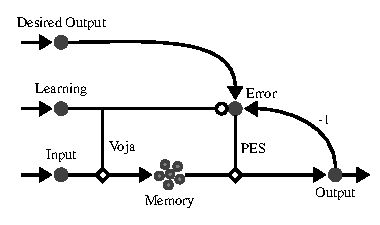
\includegraphics{voja-associative-network}
  \caption{Heteroassociative memory network using both PES and Voja learning rules.}
  \label{fig:voja-associative-network}
\end{figure}

We now proceed by applying both supervised and unsupervised learning to a single population in order to construct a network that can learn associations between pairs of vectors online.
This {\it heteroassociative memory} network is akin to a distributed hash table, in which distinct input vectors are associated with arbitrary output vectors.
The NEF has already been used to build a static memory that can recall \numprint{117659} associations between pairs of 512-dimensional vectors, using over \numprint{2500000} spiking neurons in a single layer~\citep{crawford2015}.
This model was used to traverse the relations in WordNet, a human-scale semantic network.
The output vectors can also be learned online by using the supervised PES rule to minimize the error between the output of the memory and the desired vector.
However supervised learning on its own is inadequate if we lack prior knowledge of the possible inputs to the network. If two distinct inputs cause the same neuron to fire then their two output vectors will depend on one another.
% By "inadequate", we mean that in theory one can still do it without Voja, but there is a lot of wasted space when setting the intercepts to prevent all overlap (not the same as setting the intercepts to prevent collisions), and the firing rates will be too low for most neurons. So it does not scale (unpublished?).
In the case when we cannot assume nearby inputs are associated with similar outputs we require a sparse encoding of the input vectors such that any given neuron will fire in response to at most one distinct input.
Sparse coding has been commonly observed in the hippocampus, where as few as 50 to 200 cells may participate in the encoding of a single representation \citep{Quiroga2012, Mainetti2015}.
This kind of sparsity may be achieved by using the unsupervised Voja rule to tune the encoders of the memory towards its inputs~\citep{voelker2014a} as shown in \figurename~\ref{fig:plasticity_nef/voja_encoders}.
%However, when using a traditional hardware architecture, we cannot expect to learn over 100,000 associations within a single simulation in any reasonable length of time.
%We also need lower dimensionality to run on SpiNNaker

To construct this network, we let $M$, $D$, and $K$ correspond to the number of associations, dimensionality, and the number of neurons per association, respectively.
We initialize the encoders of all $N = M \times K$ neurons using the {\it Sobol sequence} to generate a low-discrepancy set of points on the $(D-1)$-cube~\citep{Sobol1967}, and then use the inverse distribution and spherical coordinate transformation derived by \citet{fang1994} to map this sequence onto the uniform $D$-sphere.

We set $\alpha_i$ and $\beta_i$ from (\ref{eq:encoding}) such that the maximum firing rate of each neuron is $r_i$ (achieved when the input is equal to the encoder) and firing occurs with probability $\frac{1}{M}$.
This is accomplished by solving the system of equations,

\begin{align}
  \alpha_i c + \beta_i &= J_i^{0} \label{eq:firing-min} \\
  \alpha_i + \beta_i &= J_i^{max} \label{eq:firing-max} \\
  1 - F_D(c) &= \frac{1}{M} ,     \label{eq:intercept} % c &= F_D^{-1}(1 - \frac{1}{M})
\end{align}
%
where $J_i^0$ is the smallest constant input current to $G_i \left[ \cdot \right]$ that results in firing, $J_i^{max}$ is the current that produces a firing rate of $r_i$, and $F_D$ is given by the cumulative distribution:
%
\begin{equation}
  \label{eq:cosine}
  F_D(c) \propto \int_{-1}^c (1 - y^2)^{\frac{D - 3}{2}} \, dy, \quad |c| \le 1 .
\end{equation}
%
This distribution corresponds to the dot product of any unit vector with a uniformly chosen $D$-dimensional encoder.
By (\ref{eq:firing-min}), the $i^\mathrm{th}$ neuron will fire in response to a unit input $\V{x}$ if and only if $\V{e}_i \cdot \V{x} \ge c$.
Therefore, (\ref{eq:intercept}) guarantees that $N / M = K$ neurons are expected to fire in response to any unit vector.

The chosen value of $c$ also determines the maximum allowable similarity between two input vectors.
For any two distinct input vectors $\V{x}_i$ and $\V{x}_j$, we require $\V{x}_i \cdot \V{x}_j < c$ for all $i \ne j$.
Otherwise, an encoder that converges to $\V{x}_i$ with Voja will still fire in response to the input $\V{x}_j$, and vice-versa.
Whenever this occurs, the current association will overwrite the previously learned value.
The task of enforcing a maximum similarity is connected to the {\it kissing problem}~\citep{Conway1999}.
The {\it Leech lattice} gives us an optimal solution that is straightforward to compute for $D=24$.
In particular, we choose our input vectors from the set of points in the lattice closest to the origin, normalized to unit length. 
There are \numprint{196560} such points on the 24-sphere, each separated by an angle of $\theta \ge \frac{\pi}{3}$.
These points are also closely related to the codewords of the linear error-correcting {\it Golay code}.
The possible input vectors may be interpreted as spherical codewords that are optimally distant from one another in Euclidean space.
This has the benefit of producing a distinct set of neural responses that are robust to the magnitude of $\|\V{x} - \V{\hat{x}}\|$, which is precisely the approximation error minimized by (\ref{eq:rmse}).
As $\V{x}_i \cdot \V{x}_j \le cos(\theta) \|\V{x}_i\| \|\V{x}_j\| = 0.5$, we require $c > 0.5$ in order to prevent collisions.
This occurs if and only if $M > (1 - F_{24}(0.5))^{-1}$ by (\ref{eq:intercept}).
Thus, we may efficiently pack a large number of associations ($\numprint{184} \le M \le \numprint{196560}$) into a $24$-dimensional space, and then use Voja to tune each neuron to fire maximally in response to at most one input.

In order to compare our SpiNNaker implementation of the PES and Voja learning rules to the reference NEF implementation~(Nengo~\citep{bekolay2014}), we simulated the heteroassociative memory network described in \S\ref{sec:memory} at scales ranging from $M=250$ to $M=2000$ on both a 48-chip SpiNNaker machine and a standard desktop PC (3GHz AMD Athlon II X3 445).

For our benchmark, we present $M$ pairs of $24$-dimensional input and output vectors to the memory, each for \SI{200}{\milli\second} during a training phase, with learning rates of $\kappa = 0.01$ and $\eta = 0.005$ for PES and Voja, respectively.
%The simulated neuron model $G_i \left[ \cdot \right]$ was chosen to be the {\it leaky integrate-and-fire} neuron with a capacitance of $\tau_{rc} = \SI{20}{\milli\second}$ and a refractory period of $\tau_{ref} = 2$\,ms.
We then tested recall by disabling learning and presenting the same sequence of input vectors to the population of neurons, each for \SI{50}{\milli\second}.

The accuracy of the system was evaluated by comparing the value at the output node of the network during recall with the output vector presented during training.
Both the SpiNNaker and reference simulator correctly recalled the output vectors with a consistent RMSE of approximately \num{0.2} at all scales.
However as Table~\ref{tab:results/memory_scale} shows, while the SpiNNaker simulations ran in real-time (\SI{0.25}{\second} per association), the time taken by the Nengo reference simulator grew quadratically -- over $150\times$ slower than real-time in the largest configuration.

\begin{table}
  \centering
  \caption{Simulation times on SpiNNaker and Nengo reference simulator}
  \label{tab:results/memory_scale}
\sisetup{table-number-alignment=right, table-figures-decimal=0}
\begin{tabular}{S S S r r}
  \toprule
  \multicolumn{2}{c}{Number of} & \multicolumn{2}{c}{Simulation time / minutes} \\
  {Associations} & {Neurons} & {SpiNNaker} & {Nengo Reference}\\
  \midrule
    250 & 12500 & 1.0 & 20.1 \\
    500 & 25000 & 2.1 & 75.5 \\
    1000 & 50000 & 4.2 & 309.0 \\
    2000 & 100000 & 8.3 & 1307.1 \\
  \bottomrule
\end{tabular}
\end{table}

The large number of afferent synapses associated with each neuron make simulating synaptic plasticity on SpiNNaker very computationally expensive.
In this paper we built on our previous work~\citep{mundy2015} to show that, by taking advantage of the factorable synaptic weight matrices used by the NEF and not simulating individual synapses, we can simulate both plastic and static spiking neural networks highly efficiently.
To demonstrate the benefits of this approach we implemented two biologically plausible learning rules on SpiNNaker and, using these, built a heteroassociative memory network that we proved to be capable of storing a human-scale semantic network.
By simulating this memory network at scales of up to \numprint{100000} neurons, we demonstrated that these two learning rules only reduce the number of neurons each SpiNNaker core can simulate by \SI{6}{\percent} and that by using SpiNNaker rather than a standard desktop PC, simulation times are reduced by over $150\times$.

\section{Dynamical Systems Benchmarks}

Compare Braindrop versus Loihi
\TODO{Running on Eric's integrator-accuracy branch}

\subsection{Integrator}

\begin{figure}
  \centering
  \begin{subfigure}{.5\textwidth}
    \centering
    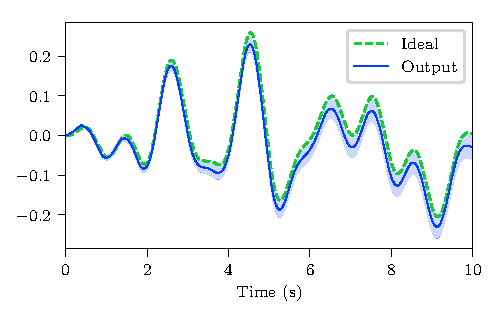
\includegraphics[width=\linewidth]{braindrop-integrator}
    \caption{Braindrop Chip}
    \label{fig:dn-braindrop}
  \end{subfigure}%
  \begin{subfigure}{.5\textwidth}
    \centering
    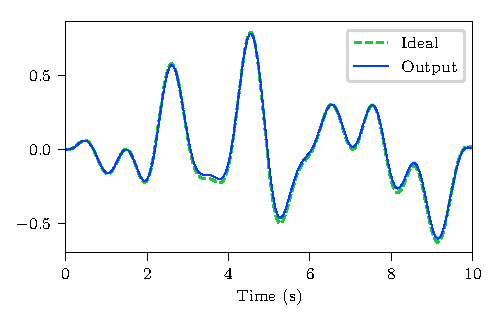
\includegraphics[width=\linewidth]{loihi-integrator}
    \caption{Loihi Emulator}
    \label{fig:dn-loihi}
  \end{subfigure}
  \caption{ \label{fig:integrator-neuromorphic}
    An integrator running on state-of-the-art neuromorphic hardware.
    The ideal solution is plotted against the mean's 95\% confidence interval, bootstrapped from $200$ trial simulations.
    (a)~Braindrop implementation, reproduced from \citet[][Figure~15]{braindrop2019}, using \numprint{1024} neurons. 
    (b)~Loihi Emulator (v0.4.0) implementation, using \numprint{256} neurons.
    See text for details.
  }
\end{figure}

The integrator, $\theta \dot{\V{x}}(t) = \V{u}(t)$, is a dynamical system used extensively by Spaun~\citep{eliasmith2012} and many other NEF and SPA models~\citep[][to name a few]{singh2004, trujillo2014a, rasmussen2017} for cognitive tasks involving working memory.
This system can persist information about the history of an input signal, starting from $t_0$ and extended indefinitely throughout time, as characterized by its solution:
$$\V{x}(t) = \V{x}(t_0) + \frac{1}{\theta} \int_{t'=t_0}^{t} \V{u}(t')\, dt' \text{.}$$
The parameter $\theta$ is a time-constant that controls how quickly the memory integrates new information.\footnote{
This parameter is useful for dimensional analysis, and when considering the transfer function, $\frac{\V{X}(s)}{\V{U}(s)} = \left( \theta s \right)^{-1}$.}
For example, beginning from an initial state of $\V{x}(t_0) = \V{0}$, if we hold the input constant at $\V{u}(t) = \V{v}$ for $\theta$ seconds ($t_0 < t \le t_0 + \theta$), and then clamp the input to $\V{u}(t) = \V{0}$ thereafter ($t > t_0 + \theta$), then $\V{x}(t) = \V{v}$ will ``store'' the vector $\V{v}$ indefinitely.
More generally, any finite set of nonlinear differential equations can be described as the integration of an input vector that is some nonlinear function of the state-vector---augmented to also include $\V{u}(t)$---as in $\theta \dot{\V{x}}(t) = \V{f}\left({\V{x}(t)}\right)$.
The nonlinearity $\V{f}(\cdot)$ may then be supported by a pool of neurons encoding the state-vector, as explained in section~\ref{sec:nef}.
Thus, the integrator is a basic component that can be used to implement more complicated nonlinear dynamical transformations, such as those involved in adaptive motor control~\citep{dewolf2016}.
We therefore use the integrator, implemented by a pool of spiking neurons using the methods of the NEF, as a benchmark for evaluating the ability of neuromorphic hardware to implement nonlinear dynamical systems.

In Figure~\ref{fig:integrator-neuromorphic}, we instantiate a one-dimensional integrator ($\theta = 1$\,s) on both Braindrop (1024 neurons) and Loihi (256 neurons).\footnote{
We use four times fewer neurons on Loihi versus Braindrop, as increasing the pool size leads to a bug in the \texttt{nengo-loihi}~v0.4.0 software.}
In both cases, the input signal is a white-noise test signal, band-limited to $1$\,Hz.
Both the ideal and the spiking activity are filtered with a lowpass ($\tau = 200$\,ms).
On Braindrop (see Figure~\ref{fig:integrator-neuromorphic}~(a), reproduced from \citet[][Figure~15]{braindrop2019}), we compensate for the distribution of synaptic time-constants, arising from transistor mismatch in the analog circuitry, using the methods of \citet{voelker2017iscas} and section~\ref{sec:mismatch}.
The chip is configured to maximize the synaptic time-constants; the empirically measured mean is $179.3$\,ms, with a standard deviation of $53.8$\,ms.
On Loihi (see Figure~\ref{fig:integrator-neuromorphic}~(b)), we set $\tau = 200$\,ms, and use the methods of \ref{sec:linear-extensions} to discretize the integrator according to the simulation time-step ($dt = 1$\,ms).

\TODO{Also used ReLU for Loihi, and some hacking of the spike-generator.}

In either case, the 95\% confidence intervals include the ideal across nearly the entire $10$\,s simulation.
This implies that the sum of any error, whether related to spiking, representation, or otherwise, has a mean value of approximately zero.
We remark that Loihi gives much more consistent trial-to-trial results, due to the all-digital nature of the chip, and lack of temperature-induced variability.
Advanced methods that can be used to provide temperature-invariant decodes in Braindrop have been recently developed by \citet{reidpint2019}, although they require external measurements of the device's temperature, and thus were not employed by this experiment.

\subsection{Delay Network}

\begin{figure}
  \centering
  \begin{subfigure}{.5\textwidth}
    \centering
    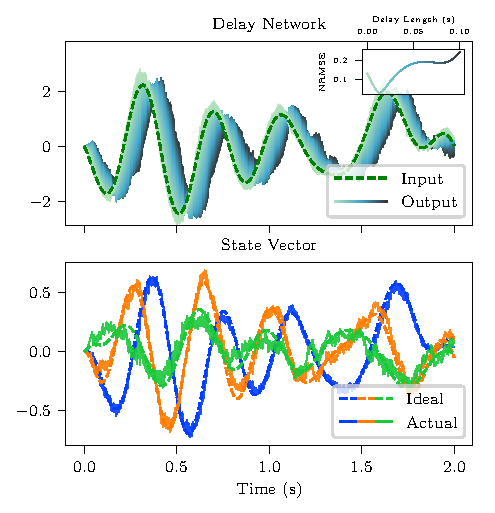
\includegraphics[width=\linewidth]{dn-braindrop}
    \caption{Braindrop Chip}
    \label{fig:dn-braindrop}
  \end{subfigure}%
  \begin{subfigure}{.5\textwidth}
    \centering
    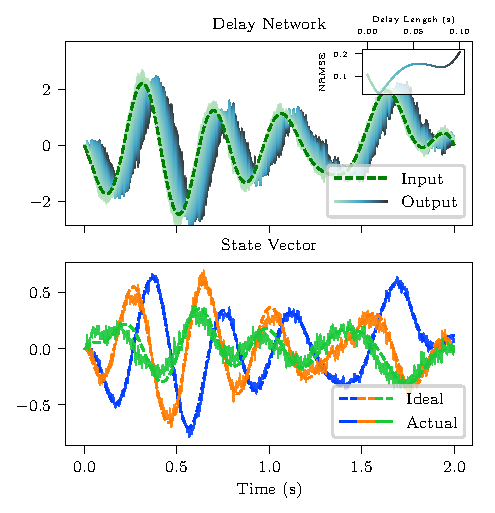
\includegraphics[width=\linewidth]{dn-loihi}
    \caption{Loihi Emulator}
    \label{fig:dn-loihi}
  \end{subfigure}
  \begin{subfigure}{\textwidth}
    \centering
    \vspace{2em}
    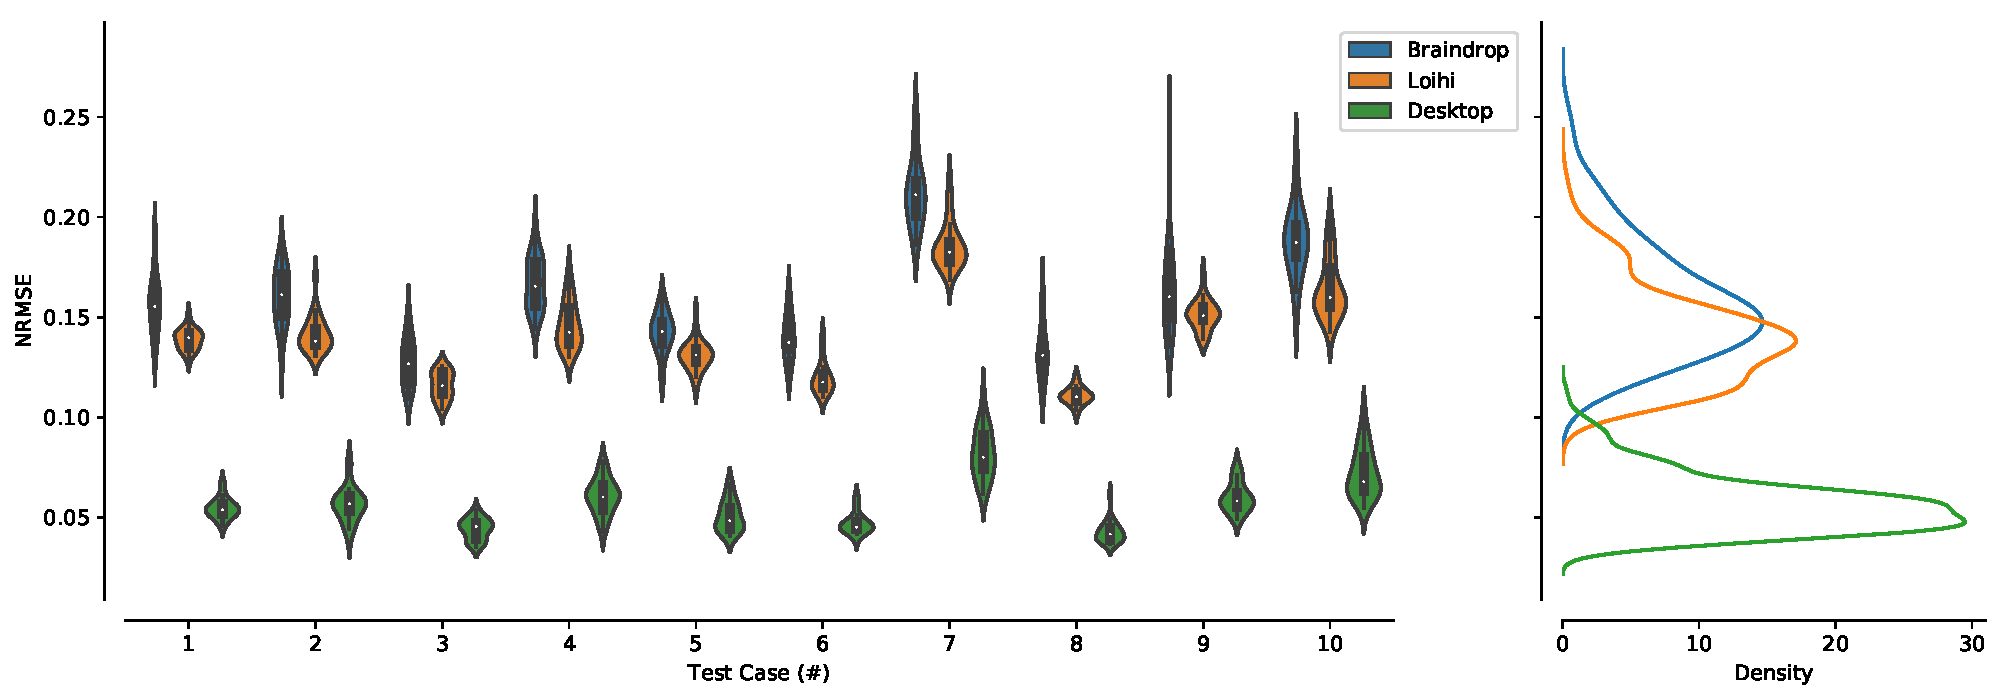
\includegraphics[width=\linewidth]{dn-trials}
    \caption{Overall Error}
    \label{fig:dn-trials}
  \end{subfigure}
  \caption{ \label{fig:dn-neuromorphic}
    Delay Network~(DN; $q=3$, $\theta=100$\,ms; chapter~\ref{chapt:delays}) running on state-of-the-art neuromorphic hardware.
    (a)~Braindrop implementation, reproduced from \citet[][Figure~16]{braindrop2019}. 
    (b)~Loihi Emulator (v0.4.0) implementation.
    (c)~Overall error~(NRMSE) for Braindrop, Loihi, and a standard desktop CPU, across 10 test cases, with 25 randomly initialized network configurations per test case.
    The simulations shown in (a) and (b) correspond to a randomly chosen trial from the first test case in (c).
    See text for details.
  }
\end{figure}


We now instantiate the same Delay Network~(DN) from chapter~\ref{chapt:delays} on state-of-the-art neuromorphic hardware (see Figure~\ref{fig:dn-neuromorphic}).
This system may be conceptualized as an entirely different kind of memory that persists not the sum of the input signal, but finite windows of input history.
In other words, the DN ``buffers'' a sliding window of the input, which enables the computation of arbitrary nonlinear transformations across the window.
This can be used as a basic building block for working memory models that must represent not only \emph{what} has occurred, but also \emph{when} it has occurred in relation to everything else.

To implement the DN, three pools, each containing $128$ spiking neurons, are recurrently coupled to each other (and to themselves), and trained to optimally buffer a white-noise test signal---band-limited to $3$\,Hz---across a $100$\,ms sliding time-window.
Output spikes are filtered using a lowpass synapse with $\tau = 20$\,ms, and weighted to decode both the state-vector and the window of history.
On Braindrop~(see Figure~\ref{fig:dn-neuromorphic}~(a), reproduced from \citet[][Figure~16]{braindrop2019}), the chip is configured to use the default distribution of synaptic time-constants (mean $\tau \approx 18$\,ms).
\TODO{Grab and plot the distribution from the calibration data using the mapped xy coordinates for the 3 ensembles.}
On Loihi~(see Figure~\ref{fig:dn-neuromorphic}~(b)), performance is maximized by using all-to-all weight matrices, and setting the recurrent time-constant to $\tau=10$\,ms.
We also compare this to the reference Nengo simulator ($\tau=10$\,ms) running on a conventional desktop CPU to obtain a baseline level of performance.
The overall error, reported as bootstrapped 95\% confidence intervals across $10 \times 25$~trials, is
[0.156,~0.163] for Braindrop,
[0.146, 0.153] for Loihi (compared to [0.145, 0.151] for the emulator), and
[0.055,~0.059] for the CPU (see Figure~\ref{fig:dn-neuromorphic}~(c)).

\chapter{Conclusions}
\label{chapt:conclusions}

We have discussed a number of theoretical and practical results involving the synthesis of dynamical systems, spiking neural networks, and neuromorphic hardware.
We now summarize our main contributions in order.

First, section~\ref{sec:sub-principles} observed a number of computational ``sub-principles'' that follow from the adoption of the NEF's three principles.
Arbitrary network topologies reduce to a single recurrently connected layer with sparse encoders and decoders with block structure isomorphic to the original graph structure.
Heterogeneous dynamical primitives form the basis for neural computation, and may be expressed within a unified language to facilitate mathematical analyses that leverage the interchangeability and composibility of such primitives.
Chaotic strange attractors emerge from even the simplest spiking implementations of such dynamical systems.
The NEF represents state-vectors by linearly projecting them onto the postsynaptic currents of neurons,  independent of any considerations of what it means to use a ``rate code'' or a ``spike-time code''.
Likewise, these state-vectors represent frequency content that grows linearly with the relative amount of energy required to drive the synapses of each postsynaptic neuron, for a fixed level of precision.

Second, section~\ref{sec:nef-suitability} addressed the suitability of NEF as a framework for compiling SNNs onto neuromorphic hardware.
Correctness is guaranteed by Theorem~\ref{thm:correctness}, which provides a novel proof of the scaling of the NEF's precision, conditioned upon a specific criteria characterizing the distribution of neural states.
Scalability is guaranteed by the previous theorem, in conjunction with a number of prior observations made about time, space, and energy requirements (Table~\ref{tab:scalability}).
Completeness is provisioned by the Turing-completeness of dynamical systems, which justifies the use of spiking neural networks---trained using the NEF to approximate the same dynamics---as powerful models of computation.
Robustness is ensured by a volume of prior work, together with our novel observation that NEF is robust to neural attractor dynamics.
Extensibility is demonstrated by a large number of Nengo backends demonstrating NEF networks functioning on a variety of seemingly disparate architectures, in addition to the extensions summarizes below.

Third, section~\ref{sec:dynamics-language} provided a number of novel perspectives on computations that are not normally viewed from a dynamical systems-based perspective.



We have discussed two main theoretical results.
The first provides a method for accurately implementing continuous-time delays in recurrent spiking neural networks.
This begins with a model description of the delay system, and ends with a finite-dimensional representation of the input's history that is mapped onto the dynamics of the synapse.
The second provides a method for harnessing a broad class of synapse models in spiking neural networks, while improving the accuracy of such networks compared to standard NEF implementations.
These extensions are validated in the context of the delay network.

Our extensions to the NEF significantly enhance the framework in two ways.
First, it allows those deploying the NEF on neuromorphics to improve the accuracy of their systems given the higher-order dynamics of mixed-analog-digital synapses~\citep{voelker2017iscas, voelker2017neuromorphic}.
Second, it advances our understanding of the effects of additional biological constraints, including finite rise-times and pure time-delays due to action potential propagation.
Not only can these more sophisticated synapse models be accounted for, but they may be harnessed to directly improve the network-level performance of certain systems.

We exploited this extension to show that it can improve the accuracy of discrete-time simulations of continuous neural dynamics.
We also demonstrated that it can provide accurate implementations of delay networks with a variety of synapse models, allowing systematic exploration of the relationship between synapse- and network-level dynamics.
Finally we suggested that these methods provide new insights into the observed temporal properties of individual cell activity.
Specifically we showed that time cell responses during a delay task are well-approximated by a delay network constructed using these methods.
This same delay network nonlinearly encodes the history of an input stimulus across the delay interval (i.e.,~ a rolling window) by compressing it into a $q$-dimensional state, with length scaling as $\bigoh{ \frac{q}{f} }$, where $f$ is the input frequency.

While we have focused our attention on delay networks in particular, our framework applies to any linear time-invariant system.
As well, though we have not shown it here, as with the original NEF formulation these methods also apply to nonlinear systems.
As a result, these methods characterize a very broad class of combinations of synapse- and network-level spiking dynamical neural networks.

\section{Future Directions}

Many important questions still remain concerning the interactions between Principles~1,~2, and~3.
While the error in our transformations scale as $\bigoh{ \frac{1}{\sqrt{n}} }$ due to independent spiking, it has been shown that near-instantaneous feedback may be used to collaboratively distribute these spikes and scale the error as $\bigoh{ \frac{1}{n} }$~\citep{boerlin2013predictive, thalmeier2016learning}.
This reduction in error has potentially dramatic consequences for the efficiency and scalability of neuromorphics by reducing total spike traffic~\citep{boahen2017neuromorph}.
However, it is currently unclear whether this approach can be applied to a more biologically plausible setting (e.g.,~using neurons with refractory periods) while retaining this linear scaling property.
Similarly, we wish to characterize the network-level effects of spike-rate adaptation, especially at higher input frequencies, in order to understand the computations that are most accurately supported by more detailed neuron models.
This will likely involve extending our work to account for nonlinear dynamical primitives and subsequently harness their effects (e.g.,~bifurcations) to improve certain classes of computations.

Delay network to store and replay episode memories (temporal semantic pointer)

Venn diagram showing intersection between biology, hardware, and what is useful?

Make useful: dendritic computation, adaptation.

Encode higher-frequency information.

Encode general temporal features (e.g., extending delay network to other basis functions).

More principled energy-minimizing network construction methods

\subsection{Energy Minimization}

``Differential encoding'' (adaptation)?

Spike-thinning (accumulator on BrainDrop)

Improving scaling by spreading out the spikes (inspired by Den\`eve)

Interneurons on Loihi

Other ideas: attentional routing (inhibition to the source). Dynamically adjusting firing rates from feedback error. Better automated selection of tuning curves (e.g., finding thresholds latent within the decomposition of functions)

\TODO{spike delays for minimizing PSC variability, like in Deneve's methods}

\cleardoublepage
\phantomsection
\renewcommand*{\bibname}{References}

\addcontentsline{toc}{chapter}{\textbf{References}}

\nocite{*}
\bibliographystyle{humannat}
\bibliography{phd}


\end{document}
